\documentclass[11pt,ngerman]{scrartcl}

% standard packages
\usepackage[utf8]{inputenc}  % input in UTF-8
\usepackage[T1]{fontenc}  % output in T1 fonts (westeuropäische Codierung)
\usepackage{lmodern}  % latin modern fonts
\usepackage[ngerman]{babel}  % deutsches Sprachpaket, neue Rechtschreibung

% Seitensetup
\usepackage{scrlayer-scrpage}  % Seitenformatierung durch KOMA-interne Optionen
\usepackage[top=4cm, bottom=4cm]{geometry}  % Seitengeometrie (kann durch KOMA ersetzt werden, hab ich aber nicht geschafft)
\usepackage[hypcap=false]{caption, subcaption}  % caption editing - hypcap warning with hyperref
\usepackage{array}  % table editing

% additional packages
\usepackage{amsmath, amssymb, amstext}  % math packages (American Math Society)
\usepackage{bm}
\usepackage{icomma}  % Kommata in Dezimalzahlen verursachen keinen Abstand mehr
\usepackage{graphicx}  % Bilder einfügen
\usepackage{float} %Bilder placement
\usepackage{pdfpages}  % PDF als vollständige Seiten einfügen
\usepackage{lastpage}  % referenziert die letzte Seite
\usepackage[separate-uncertainty=true]{siunitx}  % bessere Darstellung von Einheiten
\usepackage{makecell} %Dicke Tabellenstriche
\usepackage{longtable}
\usepackage{booktabs}
%\usepackage{datatool}
\usepackage[hidelinks]{hyperref}  % hyperref verlinkt Referenzen - hidelinks entfernt borders um links

% package setups
% Kopf- und Fußzeile durch KOMA
\pagestyle{scrheadings}  % KOMA darf entscheiden
\clearpairofpagestyles  % reset
\setkomafont{pageheadfoot}{\normalfont}  % Standardschrift in Kopf- und Fußzeile
\captionsetup{format=plain, font=small, labelfont=bf} %Better caption, Abbildung ist FETT
%\setlength{\headheight}{27.2pt}  % benötigte Höhe Kopfzeile (warning von scrlayer-scrpage, wird aber automatisch so gerendert, falls diese Option weggelassen wird)
\ihead{Interferometer}  % Kopf links %Todo Titel ändern
\chead{\textsc{Philipp} Maximilian \\ \textsc{Stark} Matthias}  % Kopf Mitte %Todo Name ändern
\ohead{15 Oktober 2021}  % Kopf rechts %Todo Datum ändern
\cfoot{\pagemark \, / \pageref{LastPage}}  % Fuß Mitte

% Table of Contents
\DeclareTOCStyleEntry{dottedtocline}{section}  % KOMA intern - Inhaltsverzeichnis mit Punkten (nur sections)

%Overbar setup
\newcommand{\overbar}[1]{\mkern 1.5mu\overline{\mkern-1.5mu#1\mkern-1.5mu}\mkern 1.5mu}
% SI
\sisetup{locale = DE}  % deutschsprachige SI-Konvention
\sisetup{quotient-mode = fraction}
\sisetup{per-mode = fraction}
\DeclareSIUnit\px{px}
\DeclareSIUnit\strich{|||}

% citation
\usepackage{csquotes}
\usepackage[backend=biber]{biblatex}
\addbibresource{interfero.bib} %Todo .bib befüllen zb.: mit JabRef (Empfehlung der Redaktion)

%Eigene Commands
\newcommand{\der}[2]{\frac{\mathrm{d}#1}{\mathrm{d}#2}}
\newcommand{\pder}[2]{\frac{\partial #1}{\partial #2}}

\begin{document}

\includepdf{Deckblatt_Stark.pdf}
\tableofcontents
\newpage

\section{Aufgabenstellung\label{Auf0}}

\begin{itemize}
	\item Im Rahmen dieses Experiments soll der Einfluss der Größe einer Lichtquelle auf das Interferenzmuster eines Doppelspalts demonstriert und erklärt werden.

	\item Zusätzlich soll der Einfluss der spektralen Breite des Lichts einer räumlich kohärenten Lichtquelle auf das Interferenzmuster eines Doppelspalts demonstriert werden.

	\item Weiters soll die Dicke einer Kunststoffschicht anhand des Interferenzmusters bestimmt werden.

	\item Zum Abschluss soll die Größe der Lichtquelle bestimmt werden, bei der für Doppelspalten mit unterschiedlichen Spaltabstand das Licht noch räumlich kohärent ist.
\end{itemize}


\section{Grundlagen}

Trifft eine monochromatische Lichtwelle auf einen Doppelspalt, so bildet diese dahinter zwei neue Elementarwellen, die sich überlagern und so Interferenzmaxima und Minima bilden. Eine beispielhafte Skizze dafür ist in \autoref{fig:1ordnung} und \autoref{fig:3ordnung} gegeben. Die Anzahl der Beugungsordnungen die abgebildet werden, hängt dabei vom Abstand der Spalten ab.

\begin{minipage}{\textwidth}
	\begin{minipage}[t]{0.5\textwidth}
		\centering
		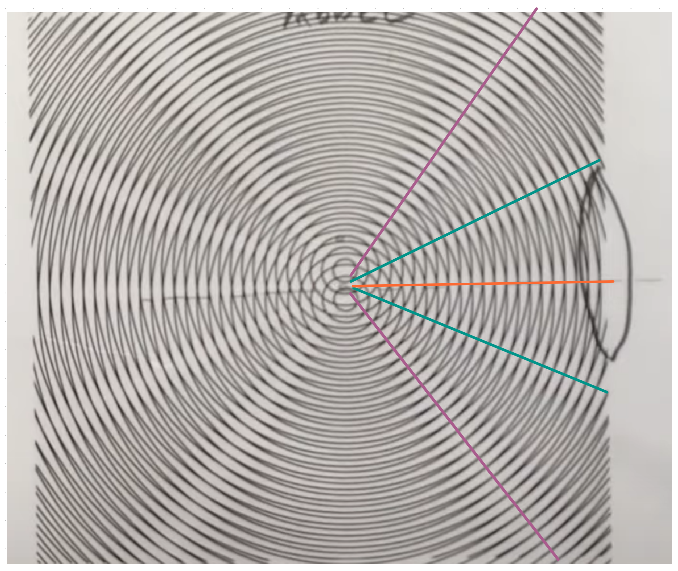
\includegraphics[width=\textwidth]{1ordnung_grenzfall}
		\captionbelowof{figure}{Abbildung der Linse bei der \newline die erste
			Beugungsordnung gerade nicht \\ mehr vom Objektiv erfasst wird
			\cite{SchweizerAbbe}}
		\label{fig:1ordnung}
	\end{minipage}
	\vspace{2mm}
	\begin{minipage}[t]{0.50\textwidth}
		\centering
		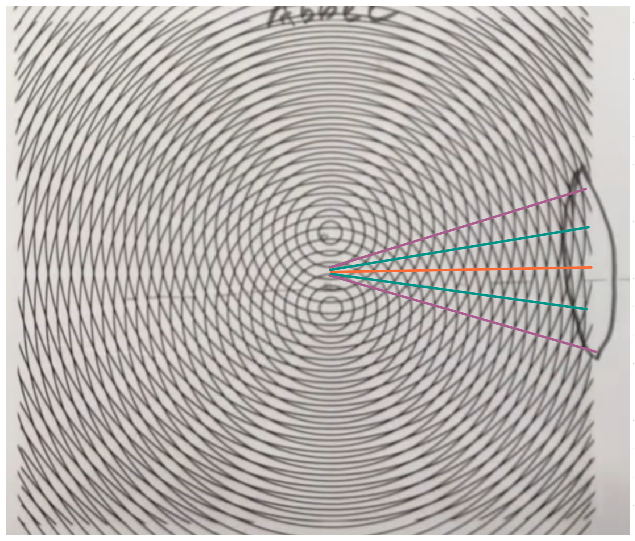
\includegraphics[width=\textwidth]{3ordnung}
		\captionof{figure}{Abbildung der Linse bei der \newline die zweite
			Beugungsordnung vom  Objektiv \\ erfasst wird \cite{SchweizerAbbe}}
		\label{fig:3ordnung}
	\end{minipage}
	\vspace{1em}
\end{minipage}

\noindent Beugungsmaxima treten bei einem bestimmten Spaltabstand $d$ immer bei Winkeln
$\theta$ auf, bei denen der Gangunterschied $\Delta s$ ein Vielfaches $m$ der
Wellenlänge $\lambda$ ist.

\begin{equation}
	\Delta s = d sin(\theta) = m \lambda
	\label{eq:wegunterschied}
\end{equation}

\noindent Reale Lichtquellen sind jedoch nie punktförmig und haben eine
Ausdehnung $2w$. $w$ steht dabei für den Abstand zur optischen Achse. Befindet
sich der beleuchtete Punkt nun abseits der optischen Achse, so wird eine
Verschiebung des Beugungsmusters sichtbar, wie in folgender \autoref{fig:pdf}
sichtbar.

\begin{center}
	\begin{minipage}[t]{\textwidth}
		\centering
		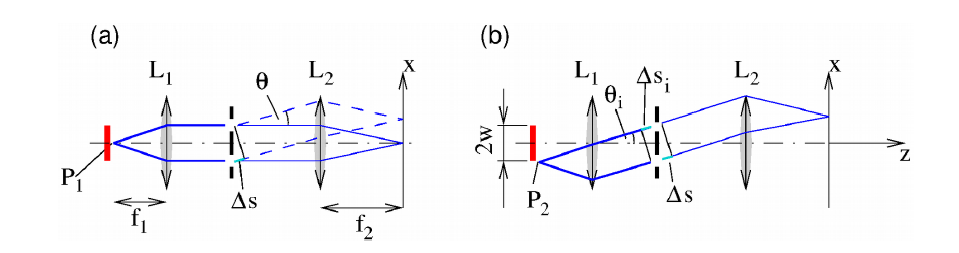
\includegraphics[width=\textwidth]{pdf}
		\captionbelowof{figure}{Strahlengang für einen Punkt der sich auf der
			optischen Achse befindet (a) und einen Punkt, der um $w$ entfernt ist.
			\cite{vorlageinterfero}}
		\label{fig:pdf}
	\end{minipage}
\end{center}

\noindent Diese Verschiebung der Interferenzmuster überlagert sich inkohärent. Ist die Lichtquelle also größer, gelangt Licht aus mehreren Richtungen in das System, wodurch der Kontrast, aufgrund von räumlicher Kohärenz, abnimmt. Anhand der Intensitätswerte kann der Kontrast $K$ nach folgender Formel berechnet werden. $I_{max}$ bezeichnet dabei die Intensität der 0. Maximums, während $I_{min}$ die Intensität der $\pm$ ersten Beugungsminimum bezeichnet.

\begin{equation}
	K = \frac{I_{max}-I_{min}}{I_{max}+I_{min}} = \Biggl|\frac{\sin(2\pi\frac{d}{\lambda}\frac{w}{f_1})}{(2\pi\frac{d}{\lambda}\frac{w}{f_1})}\Biggl|
	\label{eq:kontrast}
\end{equation}

\noindent Das erste Minimum ergibt sich dabei wenn folgende Bedingung erfüllt ist.

\begin{equation}
	2\pi\frac{d}{\lambda}\frac{w}{f_1} = \ \pi
	\label{eq:minimumbedingung}
\end{equation}

\noindent Lichtquellen mit einer Breite von 2 $w$ werden dabei als räumlich kohärent bezeichnet.

\vspace{2mm}

\noindent Neben der räumlichen Kohärenz, die aufgrund der unterschiedlichen Richtungen der Lichtwellen entsteht, gibt es auch noch zeitliche Kohärenz, die aufgrund von  unterschiedlichen Frequenzen zustande kommt.

\vspace{2mm}

\noindent Um die Schichtdicke $t$ eines Objekts zu bestimmen wird die Tatsche
verwendet, dass sich Licht in unterschiedlichen Medien verschieden schnell
ausbreitet. Zunächst wird die Position der Interferenzmaxima bestimmt. Nun wird
die zu bestimmende Schicht in den Strahlengang gegeben und der Versatz $\Delta
	s$ notiert. Die Dicke der Schicht kann dann nach folgender Formel bestimmt
werden. Dabei bezeichnet $\lambda$ die Wellenlänge des Lichts, $m$ die
entsprechenden Beugungsordnung und $n_1$ bzw. $n_2$ die Brechzahlen der
jeweiligen Medien. \cite{vorlageinterfero}

\begin{equation}
	t = \frac{m\lambda - \Delta s}{n_2-n_1}
	\label{eq:dicke}
\end{equation}

\newpage

\section{Versuchsanordnung}\label{sec:Versuchsanordnung}

\noindent Der Versuchsaufbau ist in folgender maßstabsgetreuen Skizze ersichtlich, siehe \autoref{fig:skizze}

\begin{center}
	\begin{minipage}[t]{\textwidth}
		\centering
		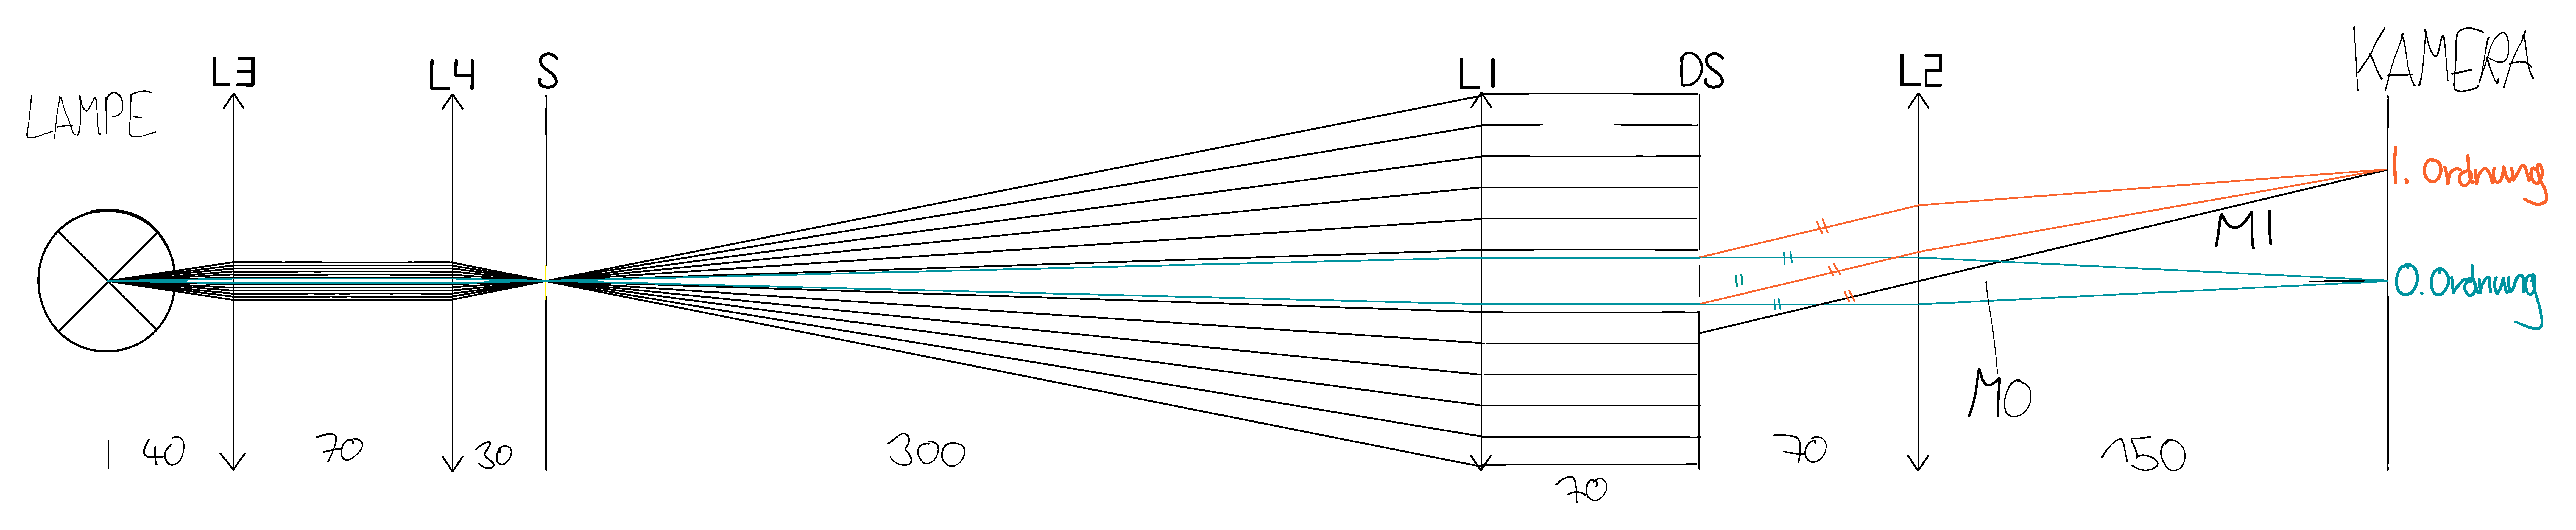
\includegraphics[width=\textwidth]{skizze}
		\captionbelowof{figure}{maßstabsgetreue Skizze des Versuchsaufbaus}
		\label{fig:skizze}
	\end{minipage}
\end{center}


\noindent L1 und L2 sind dabei die Linsen, welche das Licht der Lampe zum Spalt S bündeln. Dessen Breite kann mithilfe einer Mikrometerschraube verstellt werden. Von dort aus gelangt das Licht zur Linse L3, welche dieses parallel ausrichtet. Am Doppelspalt DS breitet sich das Licht in Form von zwei Wellen aus, die sich überlagern und so Interferenzmuster entstehen. Die Linse L3 richtet die Strahlen wieder so aus, dass diese in der Ebene der Kamera fokussiert werden. Am Filterrad F kann noch ein Filter in den Strahlengang gedreht werden. An der Stelle des blau gekennzeichneten Objekts O kann noch eine Substratschicht, sowie eine Polyacrylschickt in den Lichtweg eingeschwenkt und über einen Schraubmechanismus bewegt werden.

\noindent Der tatsächliche Versuchsaufbau ist in folgender \autoref{fig:aufbau} ersichtlich. Die einzelnen Bestandteile des Aufbaus können anhand der Skizze in \autoref{fig:skizze} bestimmt werden.

\begin{center}
	\begin{minipage}[t]{\textwidth}
		\centering
		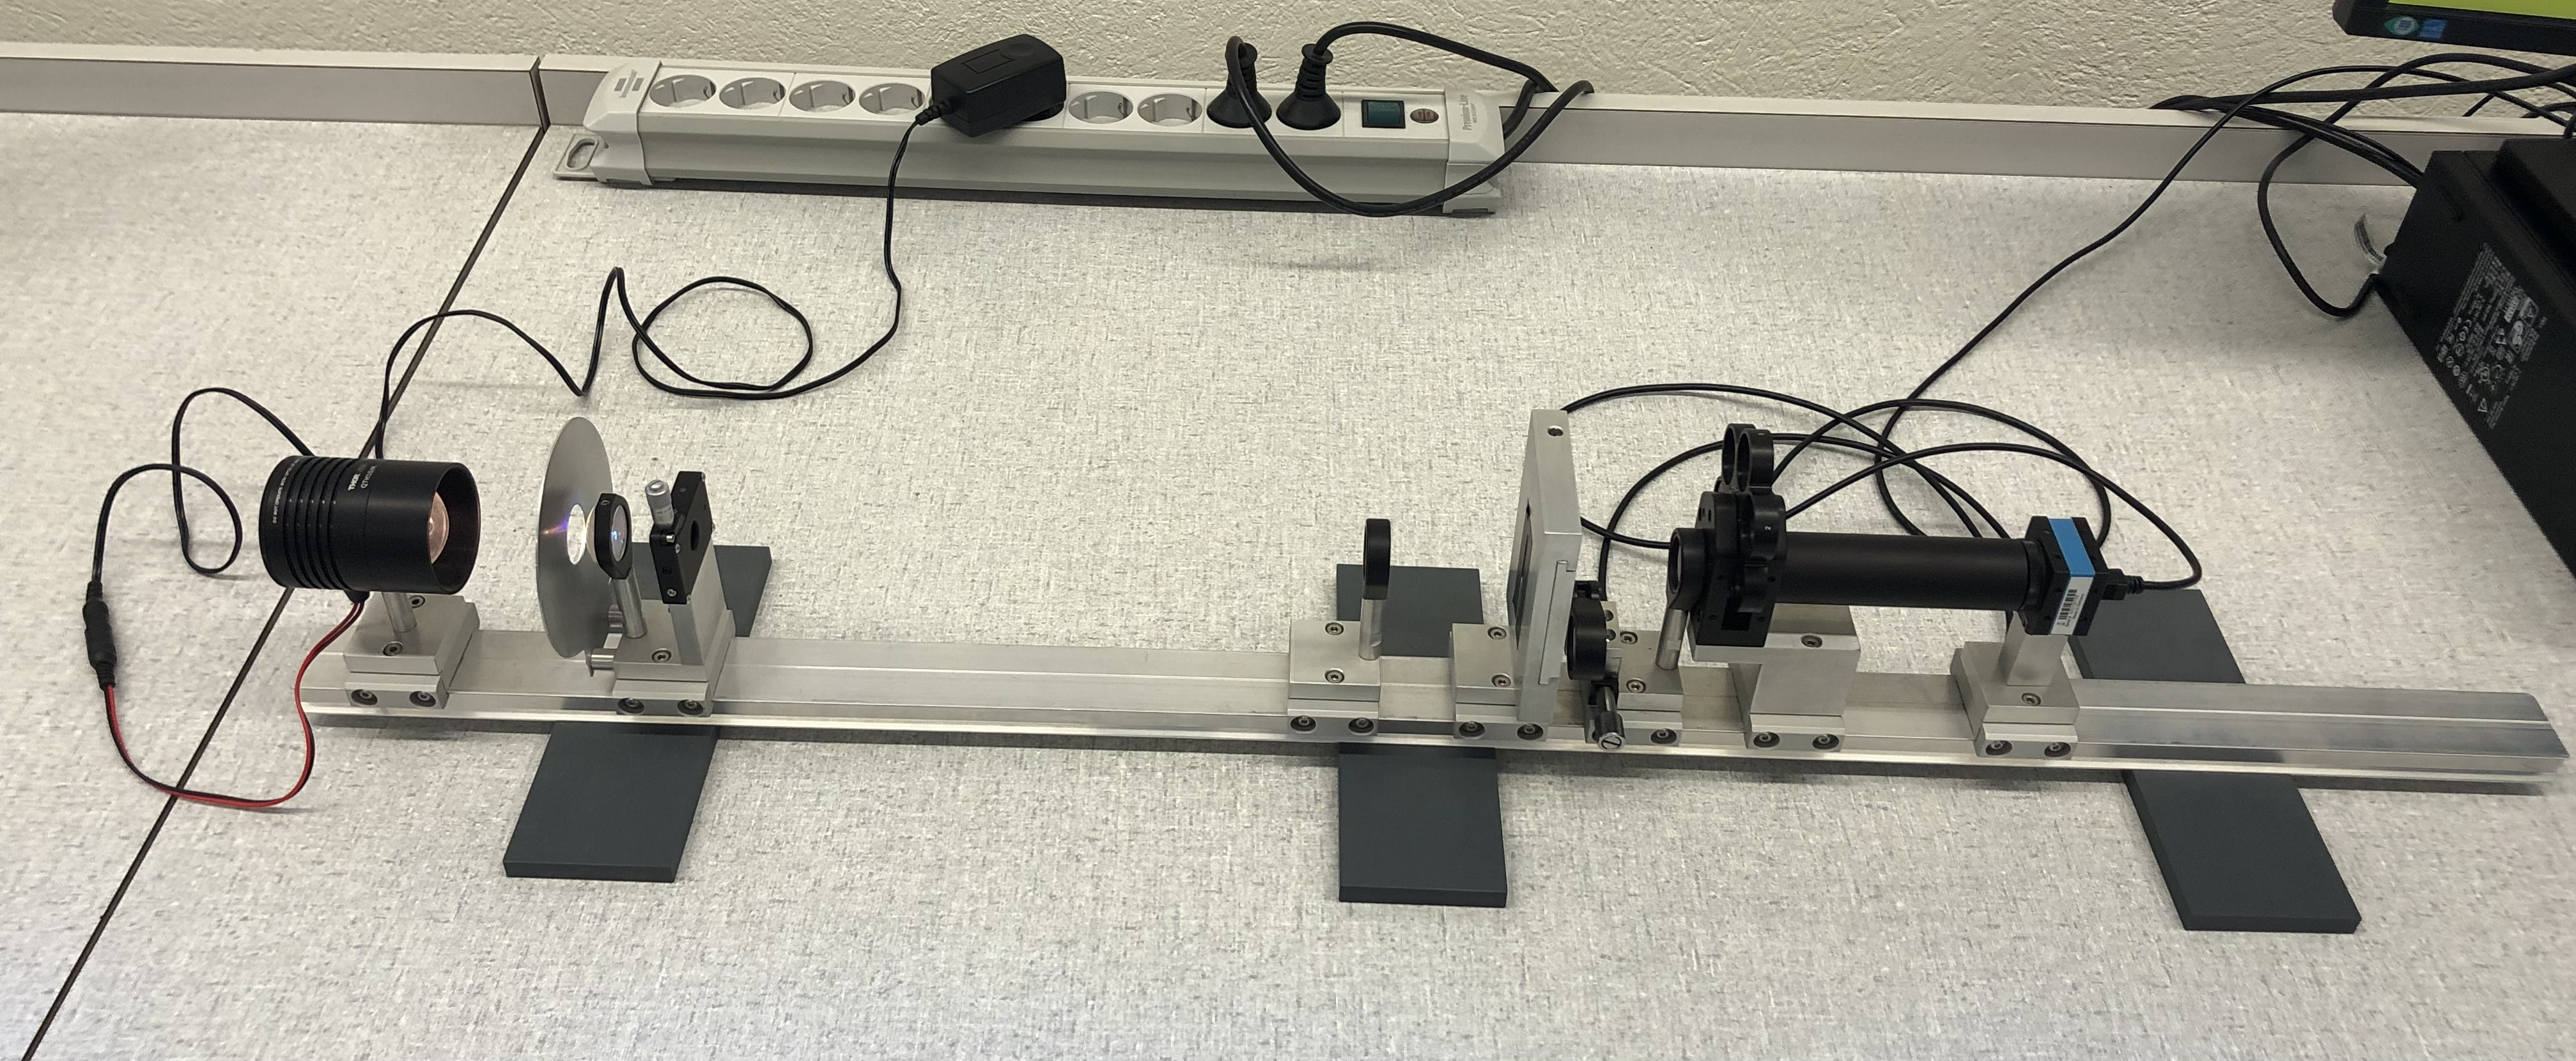
\includegraphics[width=\textwidth]{aufbau}
		\captionbelowof{figure}{Versuchsaufbau}
		\label{fig:aufbau}
	\end{minipage}
\end{center}

%Distanzen

\newpage

\section{Geräteliste}

\noindent Für die Messungen wurden folgende Geräte verwendet:

\begin{table}[H]
	\captionof{table}{Verwendete Geräte }
	\begin{center}
		\begin{tabular}{|c|c|c|c|} \hline
			\textbf{Gerät}     & \textbf{Typ}                 & \textbf{Brennweite bei Linsen} & \textbf{Hersteller} \\ \hline

			Lampe              & QTH 10 / M                   &                                & Thorlabs            \\ \hline
			Linse L3           & LMR 1 / M                    & 40mm                           & Thorlabs            \\ \hline
			Linse L4           & LMR 1 / M                    & 30mm                           & Thorlabs            \\ \hline
			Spaltblende        & FMP 1 / M                    &                                & Thorlabs            \\ \hline
			Mikrometerschraube & 148201                       &                                & Mitutojo            \\ \hline
			Linse L1           & LMR 1 / M                    & 300mm                          & Thorlabs            \\ \hline
			Doppelspalt        & 0,13 mm, 0,23 mm, 0,43 mm    &                                & Thorlabs            \\ \hline
			Objekte            & TRF 90 / M                   &                                & Thorlabs            \\ \hline
			Linse L2           & LMR 1 / M                    & 150mm                          & Thorlabs            \\ \hline
			Filterrad          & Bandpass- und Langpassfilter &                                &                     \\ \hline
			Kamera             & DMK 42 AUC 03                &                                & Imagingsource       \\ \hline
			Optische Bank      &                              &                                &                     \\ \hline
			Computersoftware   & IC Capture                   &                                &                     \\ \hline
			Computersoftware   & imageJ                       &                                &                     \\ \hline
		\end{tabular}
	\end{center}
\end{table}




\section{Versuchsdurchführung \& Messergebnisse}\label{sec:Versuchsdurchführung}

Um die genaue Spaltbreite feststellen zu können, lässt sich diese mithilfe einer Mikrometerschraube variieren. Dabei ist zu beachten, dass der Spalt bei der Nulllage der Mikrometerschraube nicht vollständig geschlossen ist, wie in \autoref{fig:spalt} ersichtlich ist.

\begin{center}
	\begin{minipage}[t]{0.5\textwidth}
		\centering
		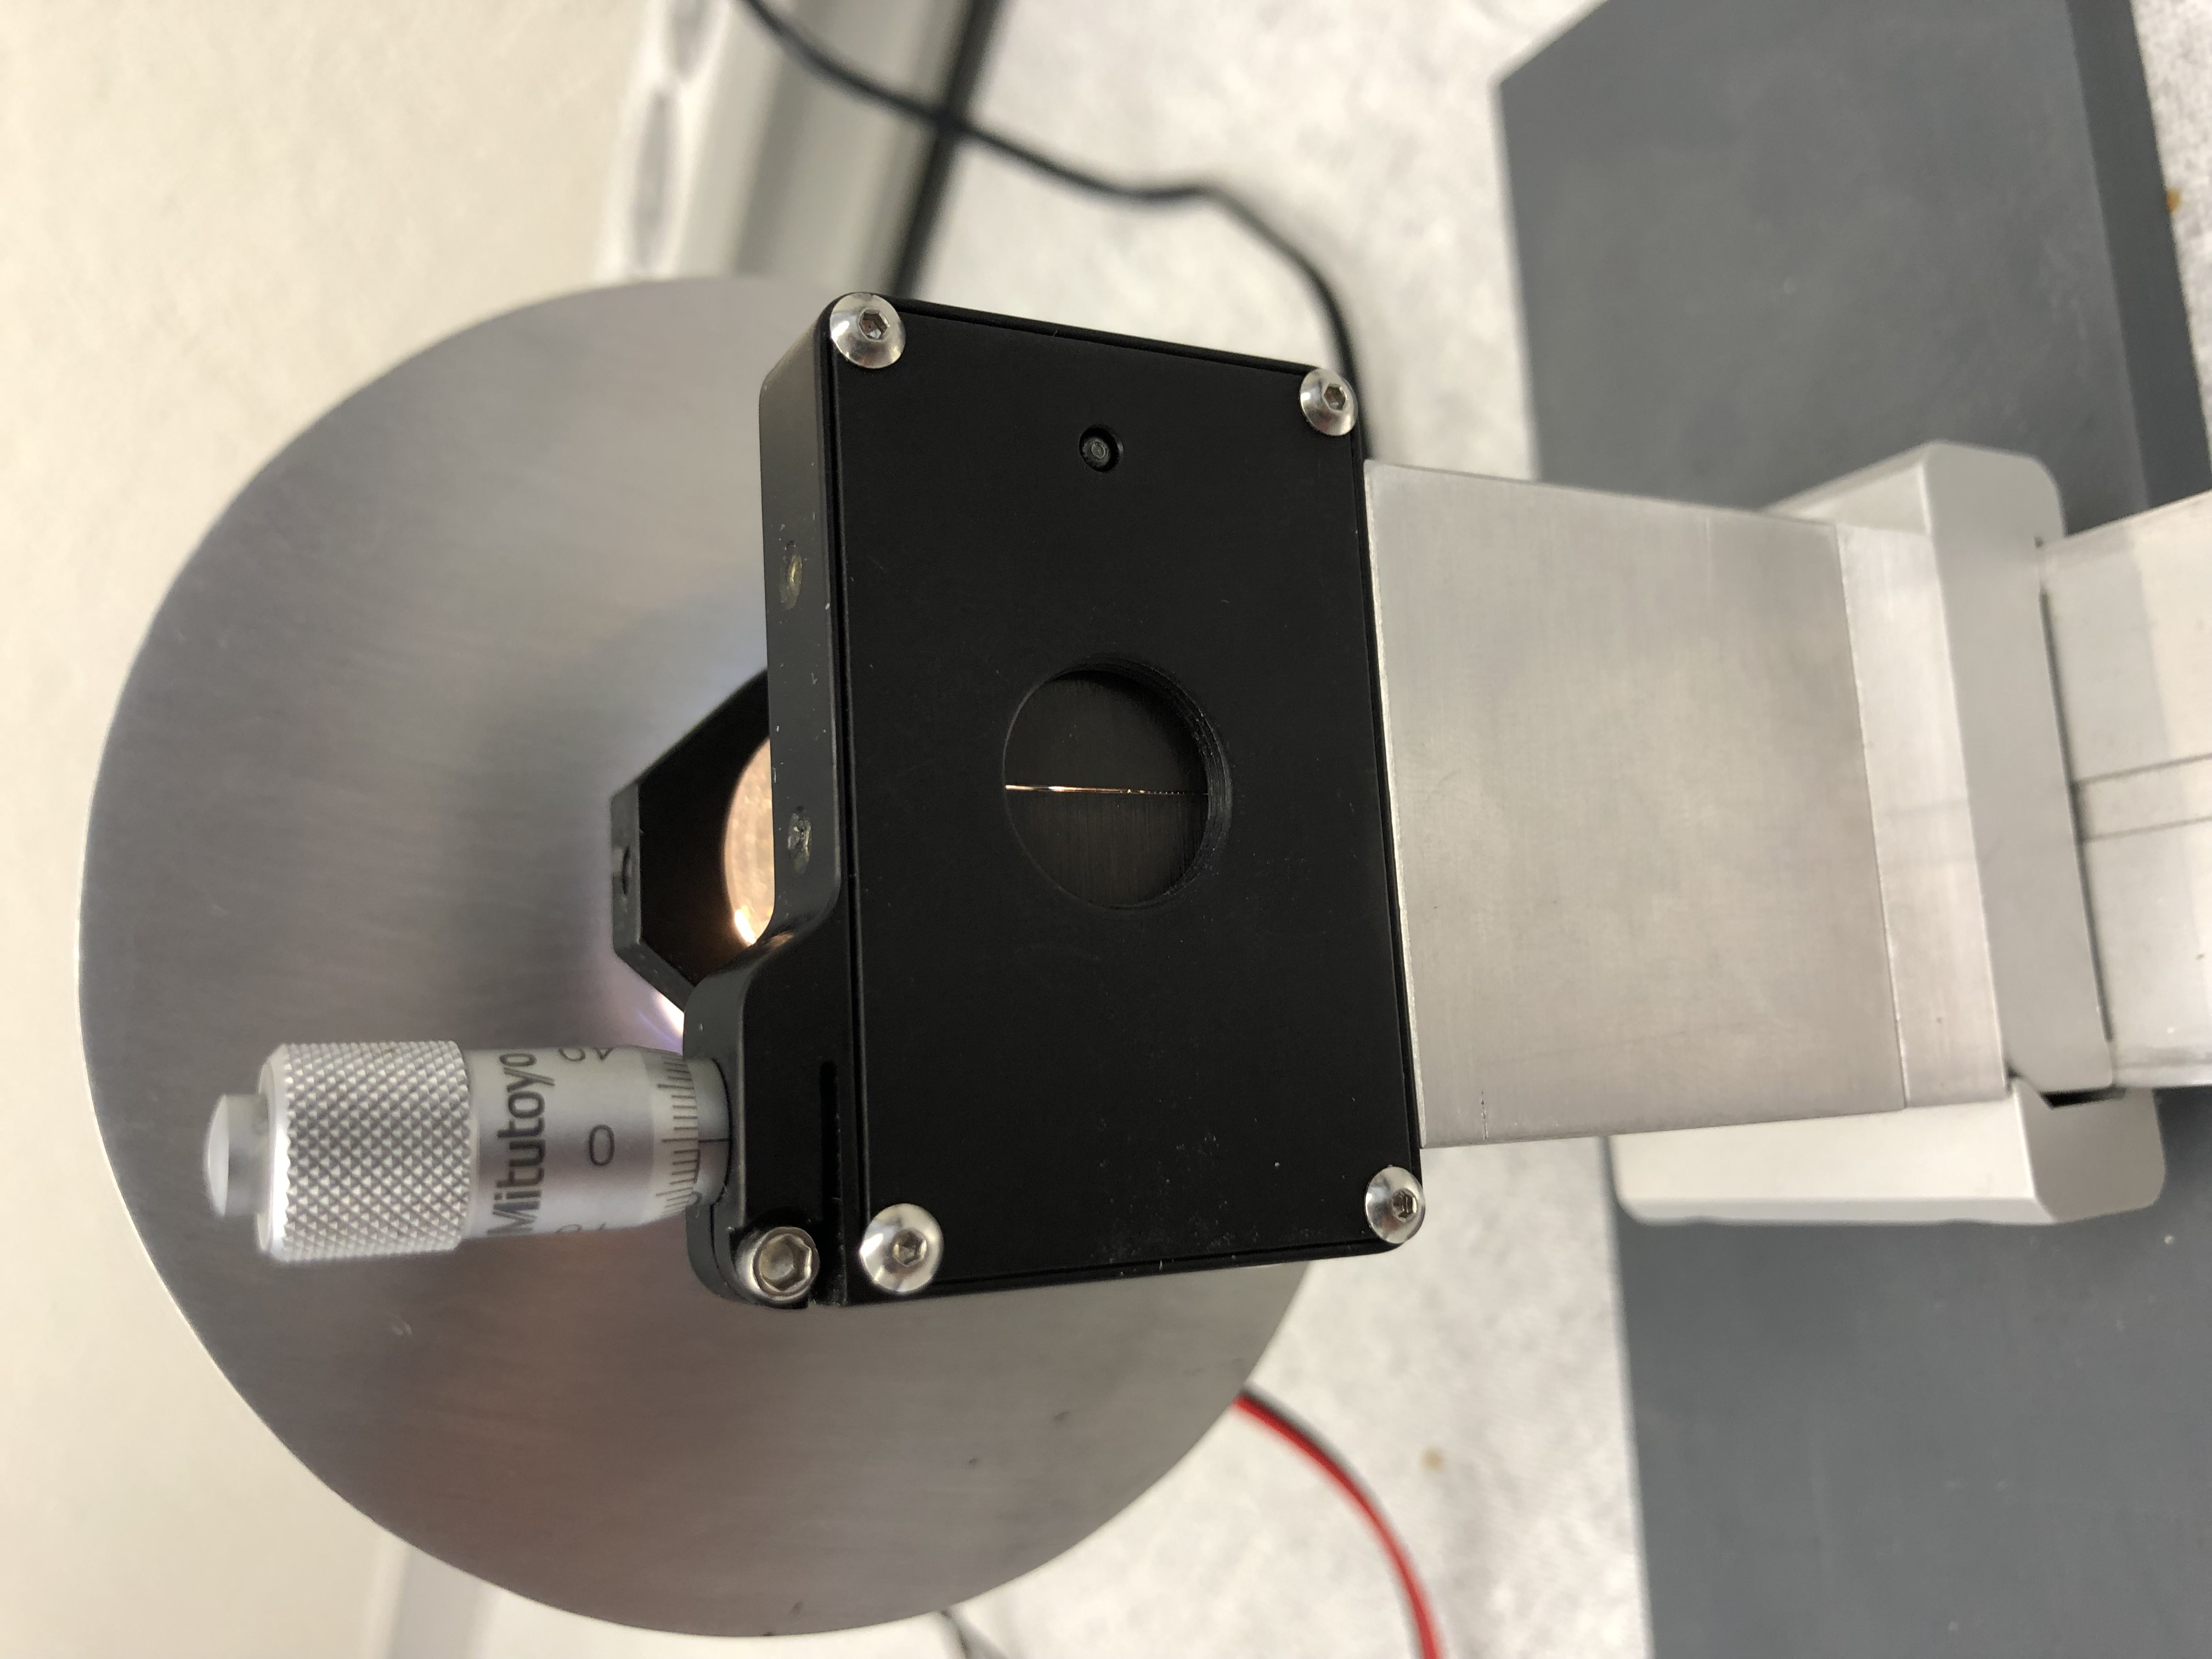
\includegraphics[angle = -90, width=\textwidth]{spalt}
		\captionbelowof{figure}{Spaltabstand bei Nullpunktslage}
		\label{fig:spalt}
	\end{minipage}
\end{center}

\noindent Um nun also den tatsächlichen Spaltabstand bestimmen zu können, wird der Spalt vollständig geschlossen und der entsprechende Wert der Mikrometerschraube abgelesen, was einen Versatz von \SI{-0.210(5)}{mm} ergibt, der bei der Auswertung berücksichtigt werden muss.


\subsection{Einfluss der Größe einer Lichtquelle auf das Interferenzmuster eines Doppelspalts}

Zunächst wird am Filterrad der Bandpassfilter für eine Wellenlänge von
\SI{633}{\nm} in den Strahlengang gedreht, um für monochromatisches Licht zu
sorgen. Bei den Doppelspalten wird der Breiteste Spalt mit einem Abstand von
\SI{0.43}{mm} verwendet.

\vspace{2mm}

\noindent Nun wird mithilfe der Computersoftware ``IC Capture`` die ``Exposure`` geändert, was der Belichtungszeit entspricht. Dabei ist zu beachten, dass am rechten Rand der angezeigten Grafik, die in \autoref{fig:graf} sichtbar ist, ein gelber Balken angezeigt wird. Dies bestätigt, dass die Belichtungsparameter richtig eingestellt sind.

\begin{center}
	\begin{minipage}[t]{0.7\textwidth}
		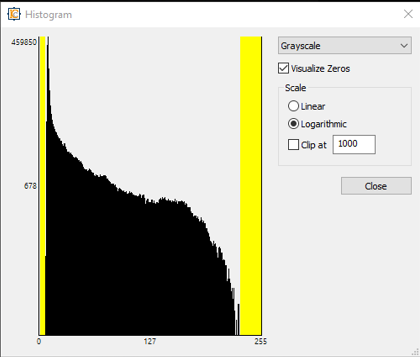
\includegraphics[width=\textwidth]{graf}
		\captionof{figure}{Grafik mit gelben Balken am Rand}
		\label{fig:graf}
	\end{minipage}
\end{center}

\noindent Wenn die Helligkeit richtig eingestellt ist, ist nun in der Software folgendes Bild aus \autoref{fig:bild} sichtbar.

\begin{center}
	\begin{minipage}[t]{0.7\textwidth}
		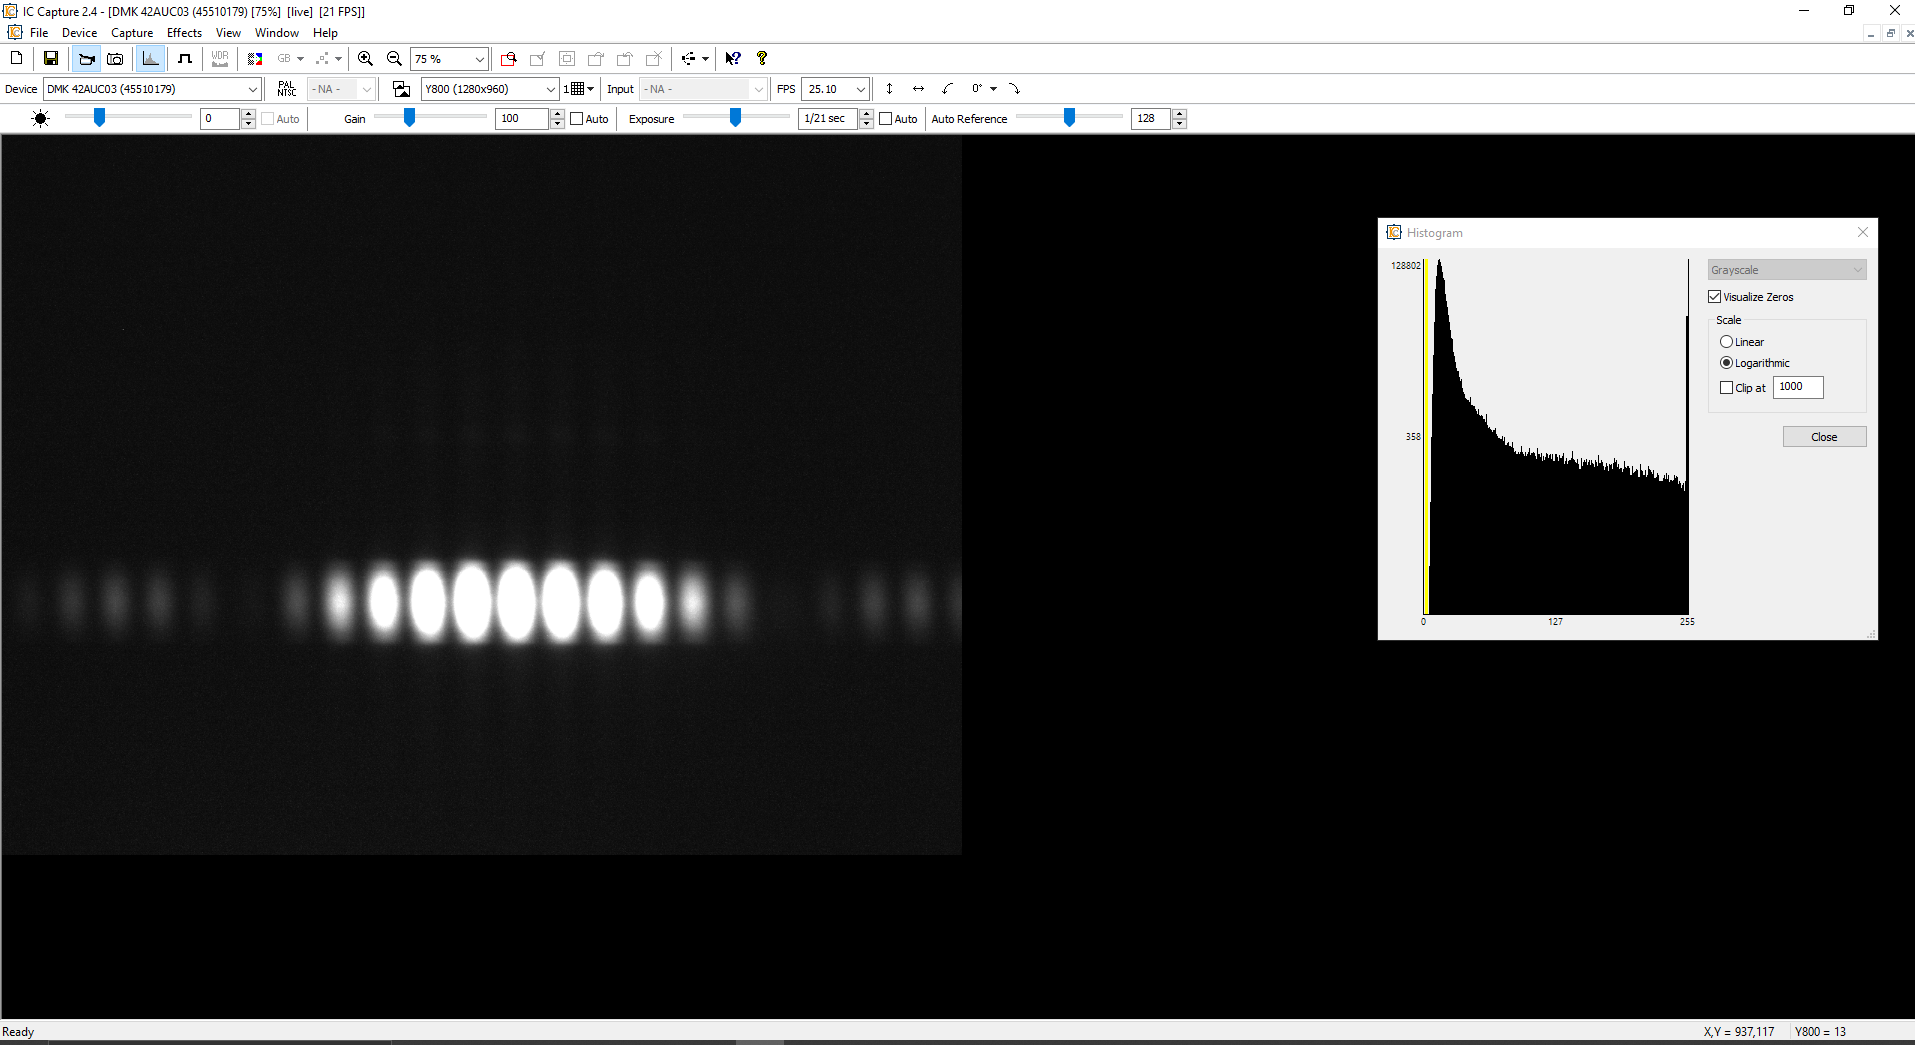
\includegraphics[width=\textwidth]{Interfero/Versuch1/viele_ordnungen}
		\captionof{figure}{Sichtbares Bild mit Beugungsordnungen}
		\label{fig:bild}
	\end{minipage}
\end{center}

\noindent Nun wird der Spalt vollkommen geschlossen und vorsichtig wieder geöffnet. Dabei wird alle \SI{0.1}{mm} ein Bild des Interferenzmusters gemacht und die entsprechende Spaltbreite notiert. Dabei ist, wie bereits erwähnt, der Offset der Mikrometerschraube zu beachten. Die Belichtungszeit muss bei jedem Spaltabstand neu nachjustiert werden, da sich mit zunehmender Größe des Spalts natürlich aus die Helligkeit der aufgezeichneten Bilder erhöht. Ein exemplarisches Bild des Interferenzmusters ist in \autoref{fig:muster_bsp} zu sehen. Der abgelesene Wert der Spaltbreite ist dabei \SI{-0.010(5)}{mm}, was unter der Berücksichtigung des Offsets einer Breite von \SI{0.200(5)}{mm} entspricht.

\begin{center}
	\begin{minipage}[t]{0.7\textwidth}
		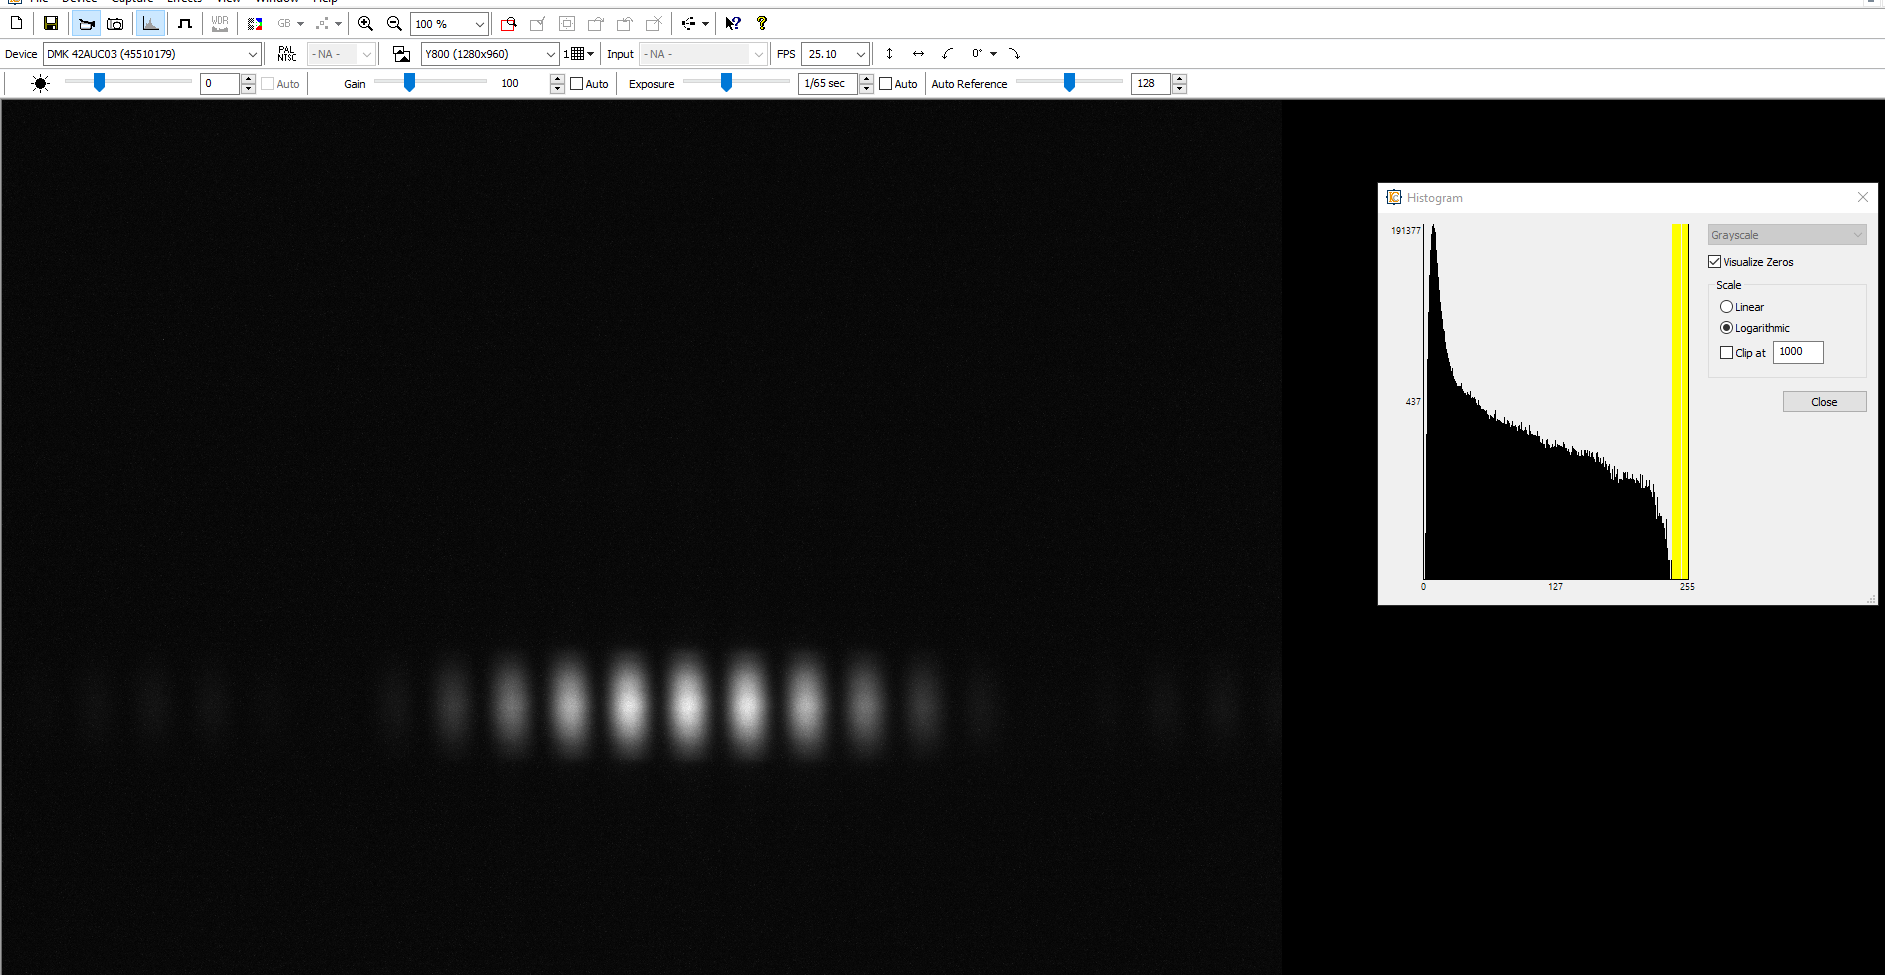
\includegraphics[width=\textwidth]{Interfero/Versuch1/-0_01konstrast}
		\captionof{figure}{Interferenzmuster bei einer Spaltbreite von \SI{0.200(5)}{mm} unter Verwendung des Bandpassfilters und einem Doppelspalt mit \SI{0.430(5)}{mm}}
		\label{fig:muster_bsp}
	\end{minipage}
\end{center}

\noindent Die so aufgenommenen Bilder wurden nun mithilfe der Bildbearbeitungssoftware ``imageJ`` ausgewertet. Dazu wird eine rechteckige Auswahl über das Bild des Beugungsmusters gelegt. Mit der ``Analyze``Funktion kann nun der Grauwert, welcher der Intensität entspricht, der jeweiligen Pixelnummer zugeordnet werden und die so erhaltenen Daten in Form einer CSV-Datei gespeichert und so geplottet werden. Dabei ist zu beachten, dass sich der Auswahlkasten über das gesamte Bild erstreckt, was später für die Bestimmung der Unsicherheit noch wichtig wird.

\vspace{2mm}

\noindent Im folgenden sind die so geplotteten Graphen für die unterschiedlichen Spaltbreiten sichtbar.

\noindent Der besseren Übersicht halber, wird beim Spaltabstand nur der Wert mit dem Berücksichtigten Offset der Mikrometerschraube notiert.

\vspace{2mm}

\begin{minipage}{\textwidth}
	\begin{minipage}[t]{0.5\textwidth}
		\centering
		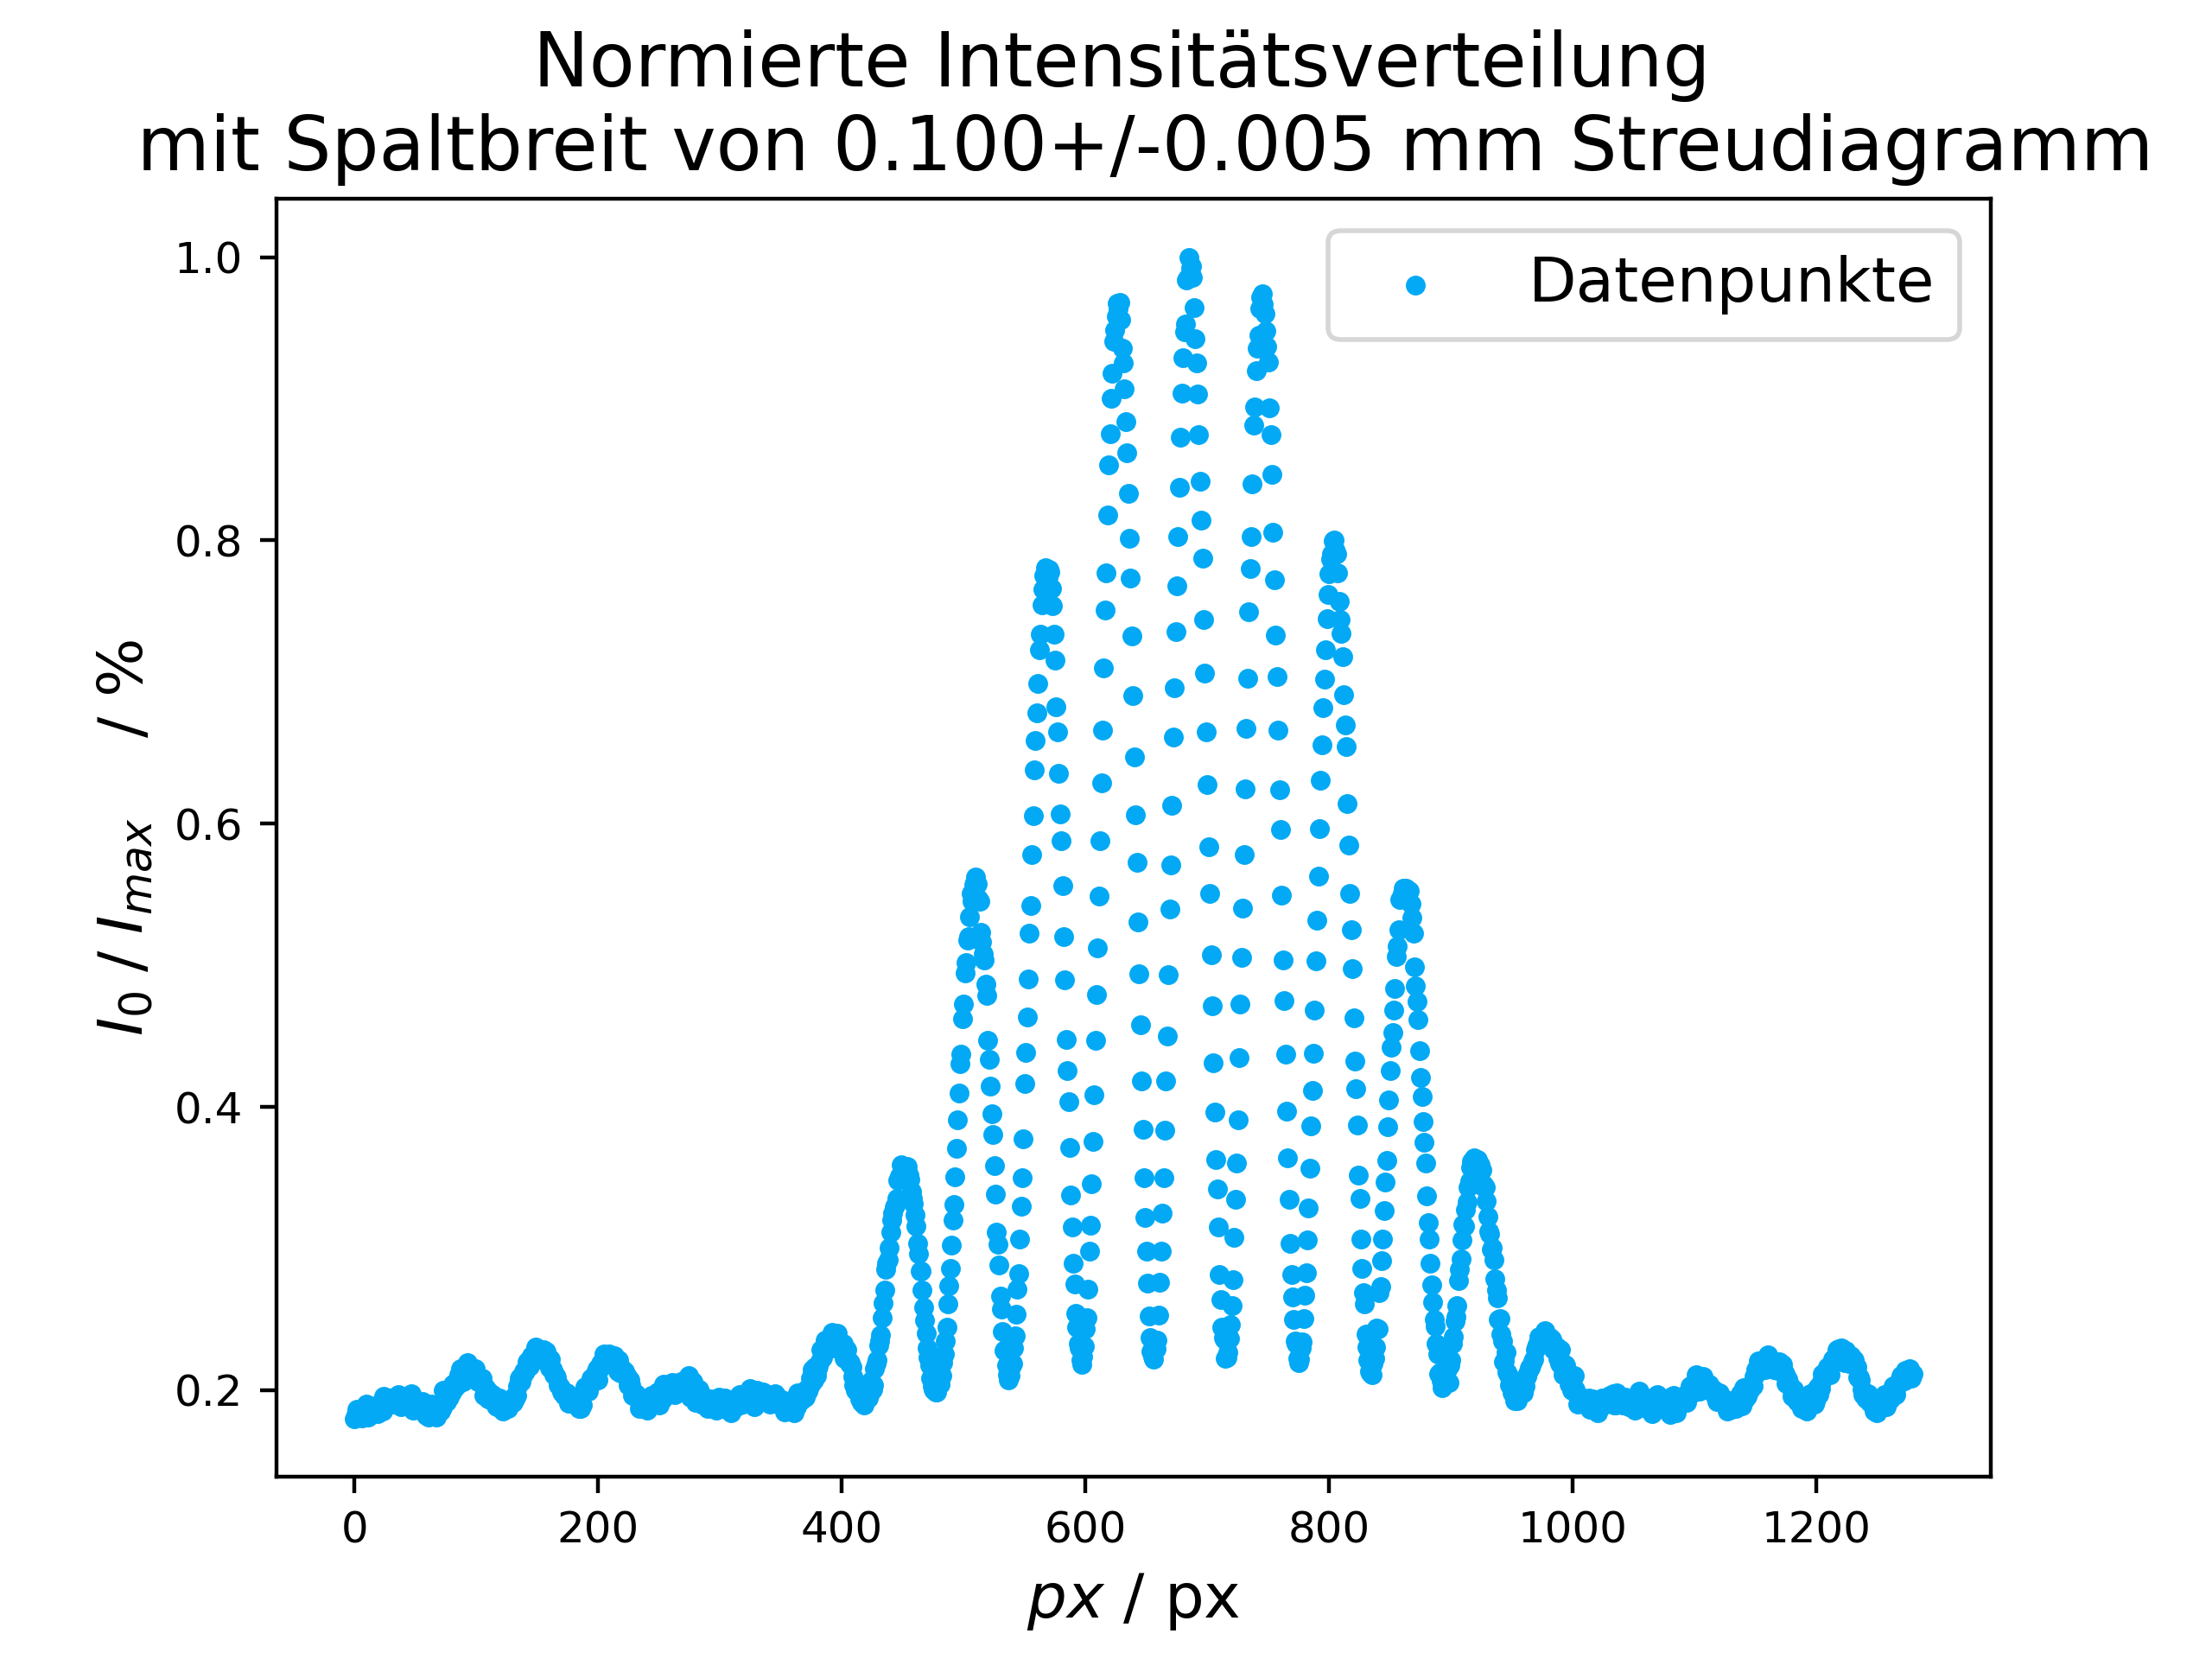
\includegraphics[width=\textwidth]{auswertung/-0_11konstrast}
		\captionbelowof{figure}{geplotteter Grauwert \\ aufgetragen zu jeweiligen Pixelnummer \\ bei einer Spaltbreite von \SI{0.100(5)}{mm}}
		\label{fig:ausreisergraph}
	\end{minipage}
	\vspace{2mm}
	\begin{minipage}[t]{0.50\textwidth}
		\centering
		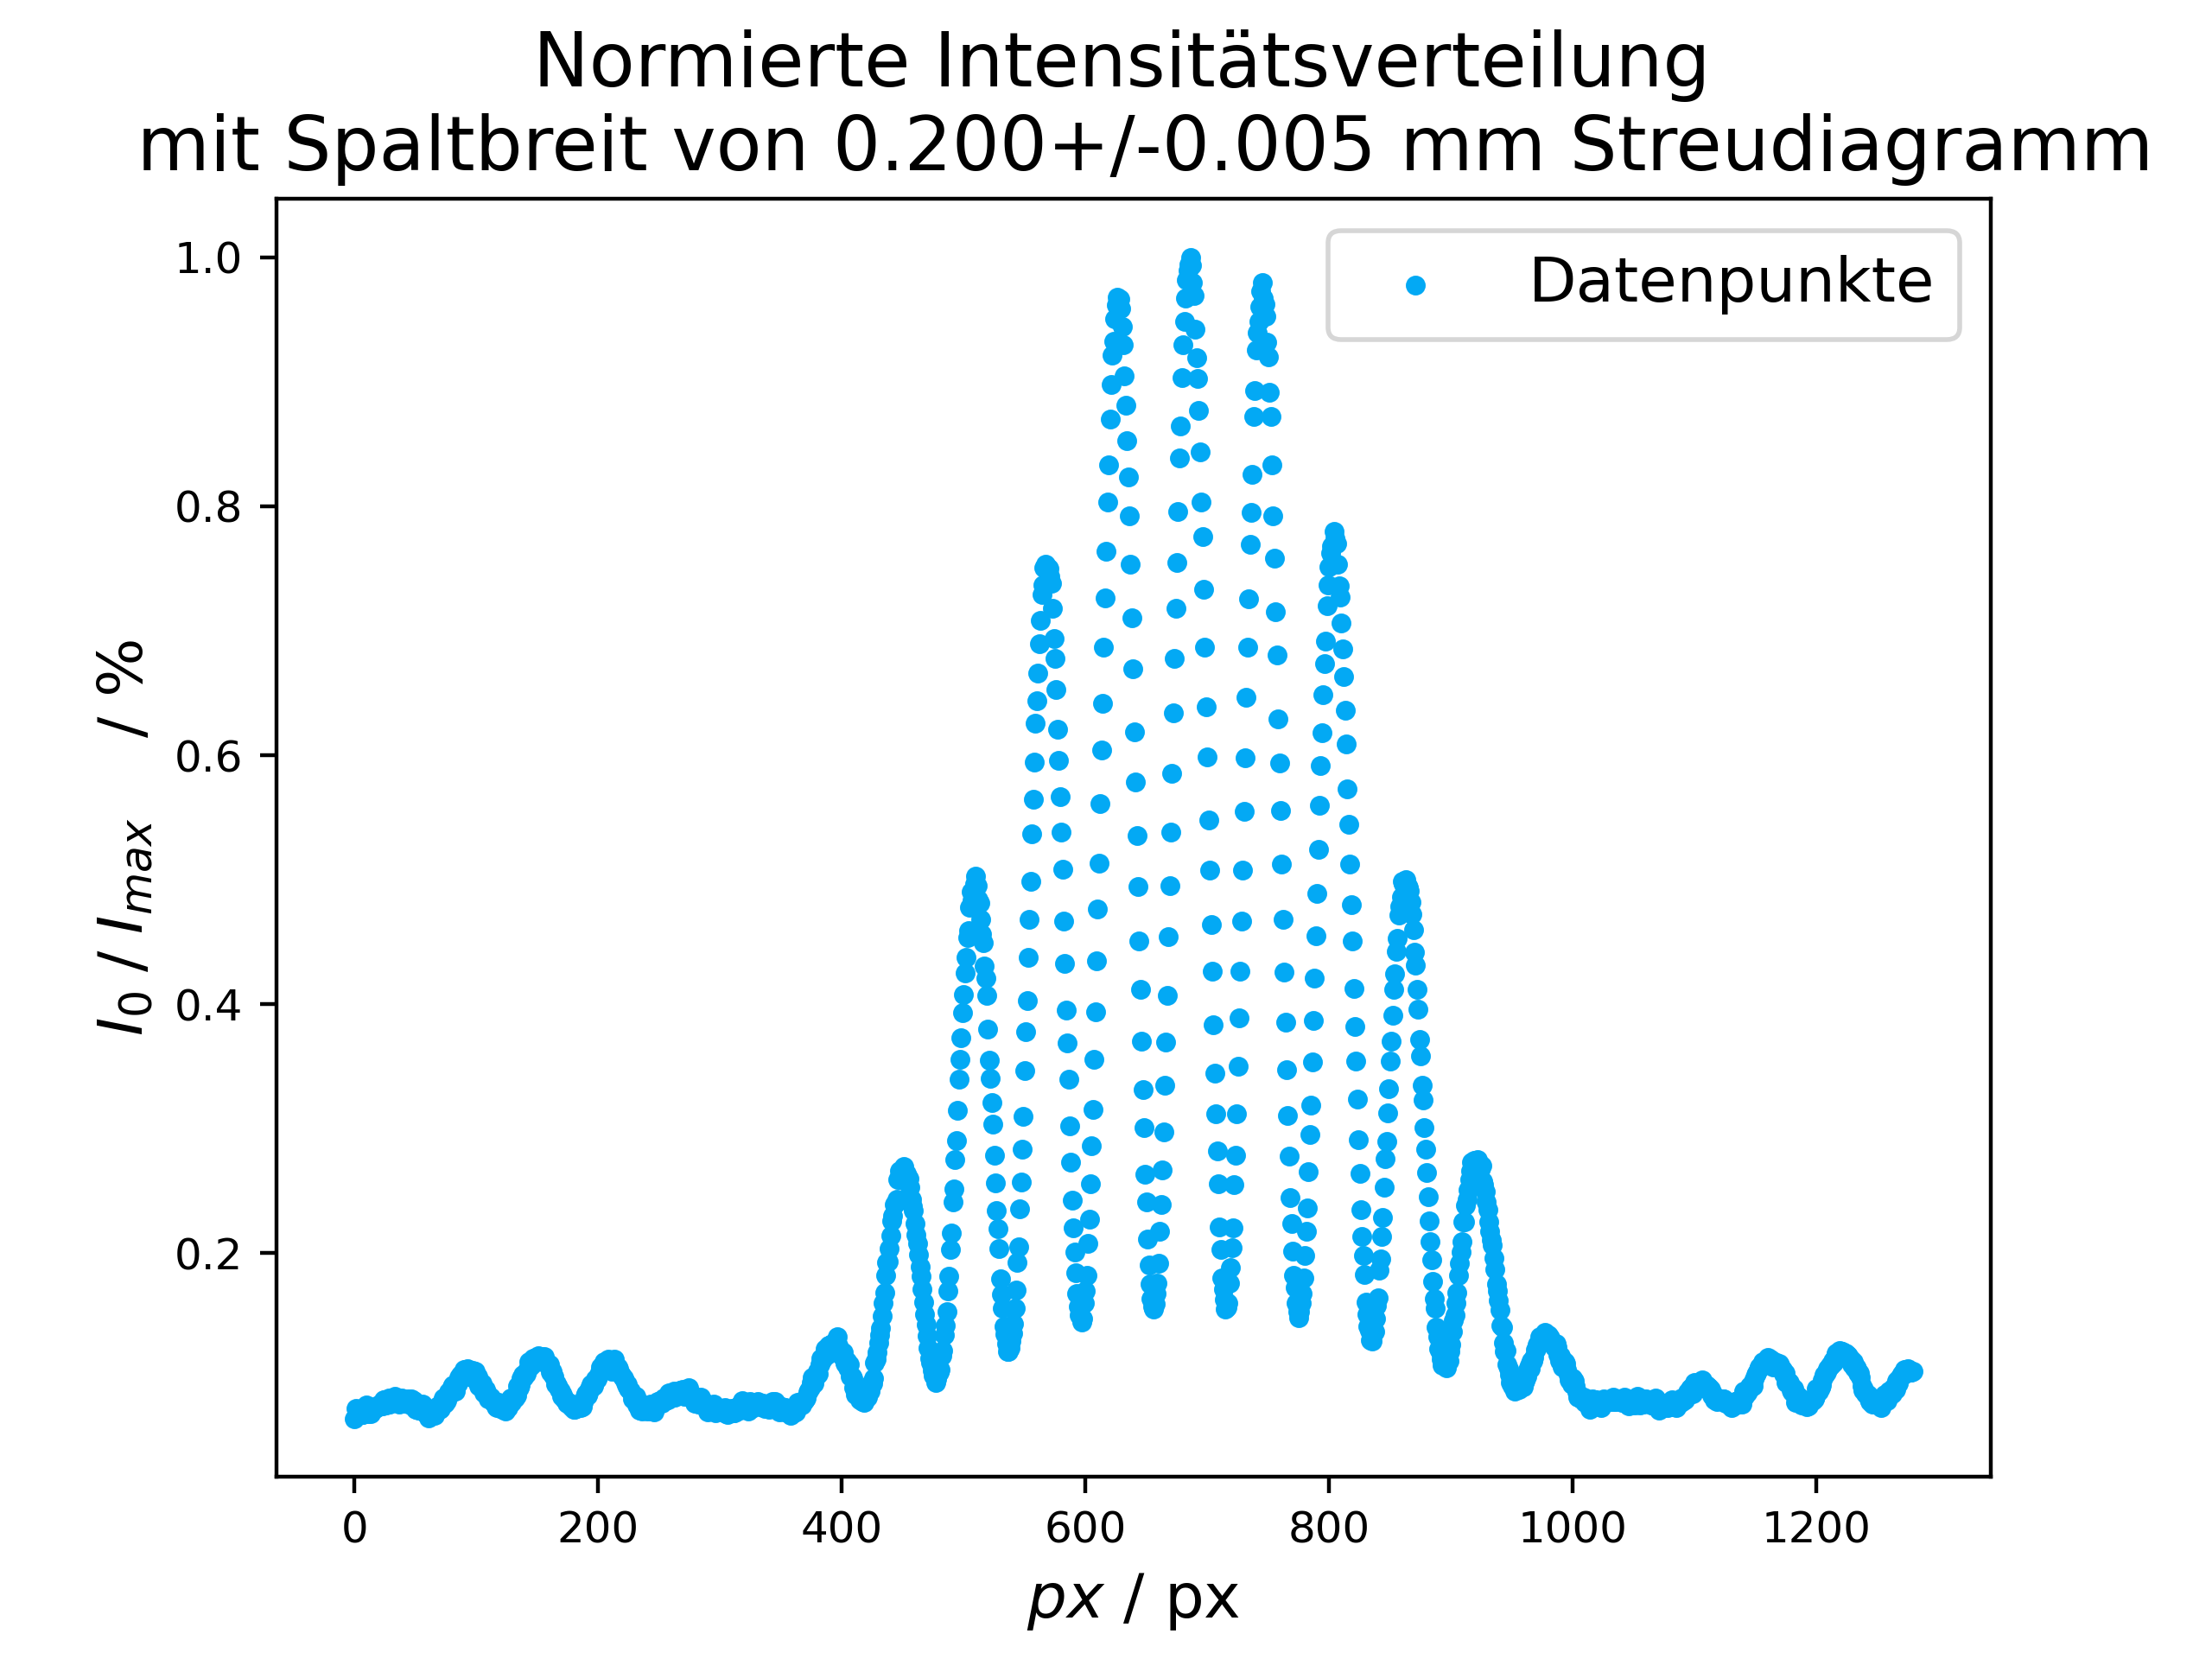
\includegraphics[width=\textwidth]{auswertung/-0_01konstrast}
		\captionof{figure}{geplotteter Grauwert \\ aufgetragen zu jeweiligen Pixelnummer \\ bei einer Spaltbreite von \SI{0.200(5)}{mm}}
	\end{minipage}
	\vspace{1em}
\end{minipage}

\begin{minipage}{\textwidth}
	\begin{minipage}[t]{0.5\textwidth}
		\centering
		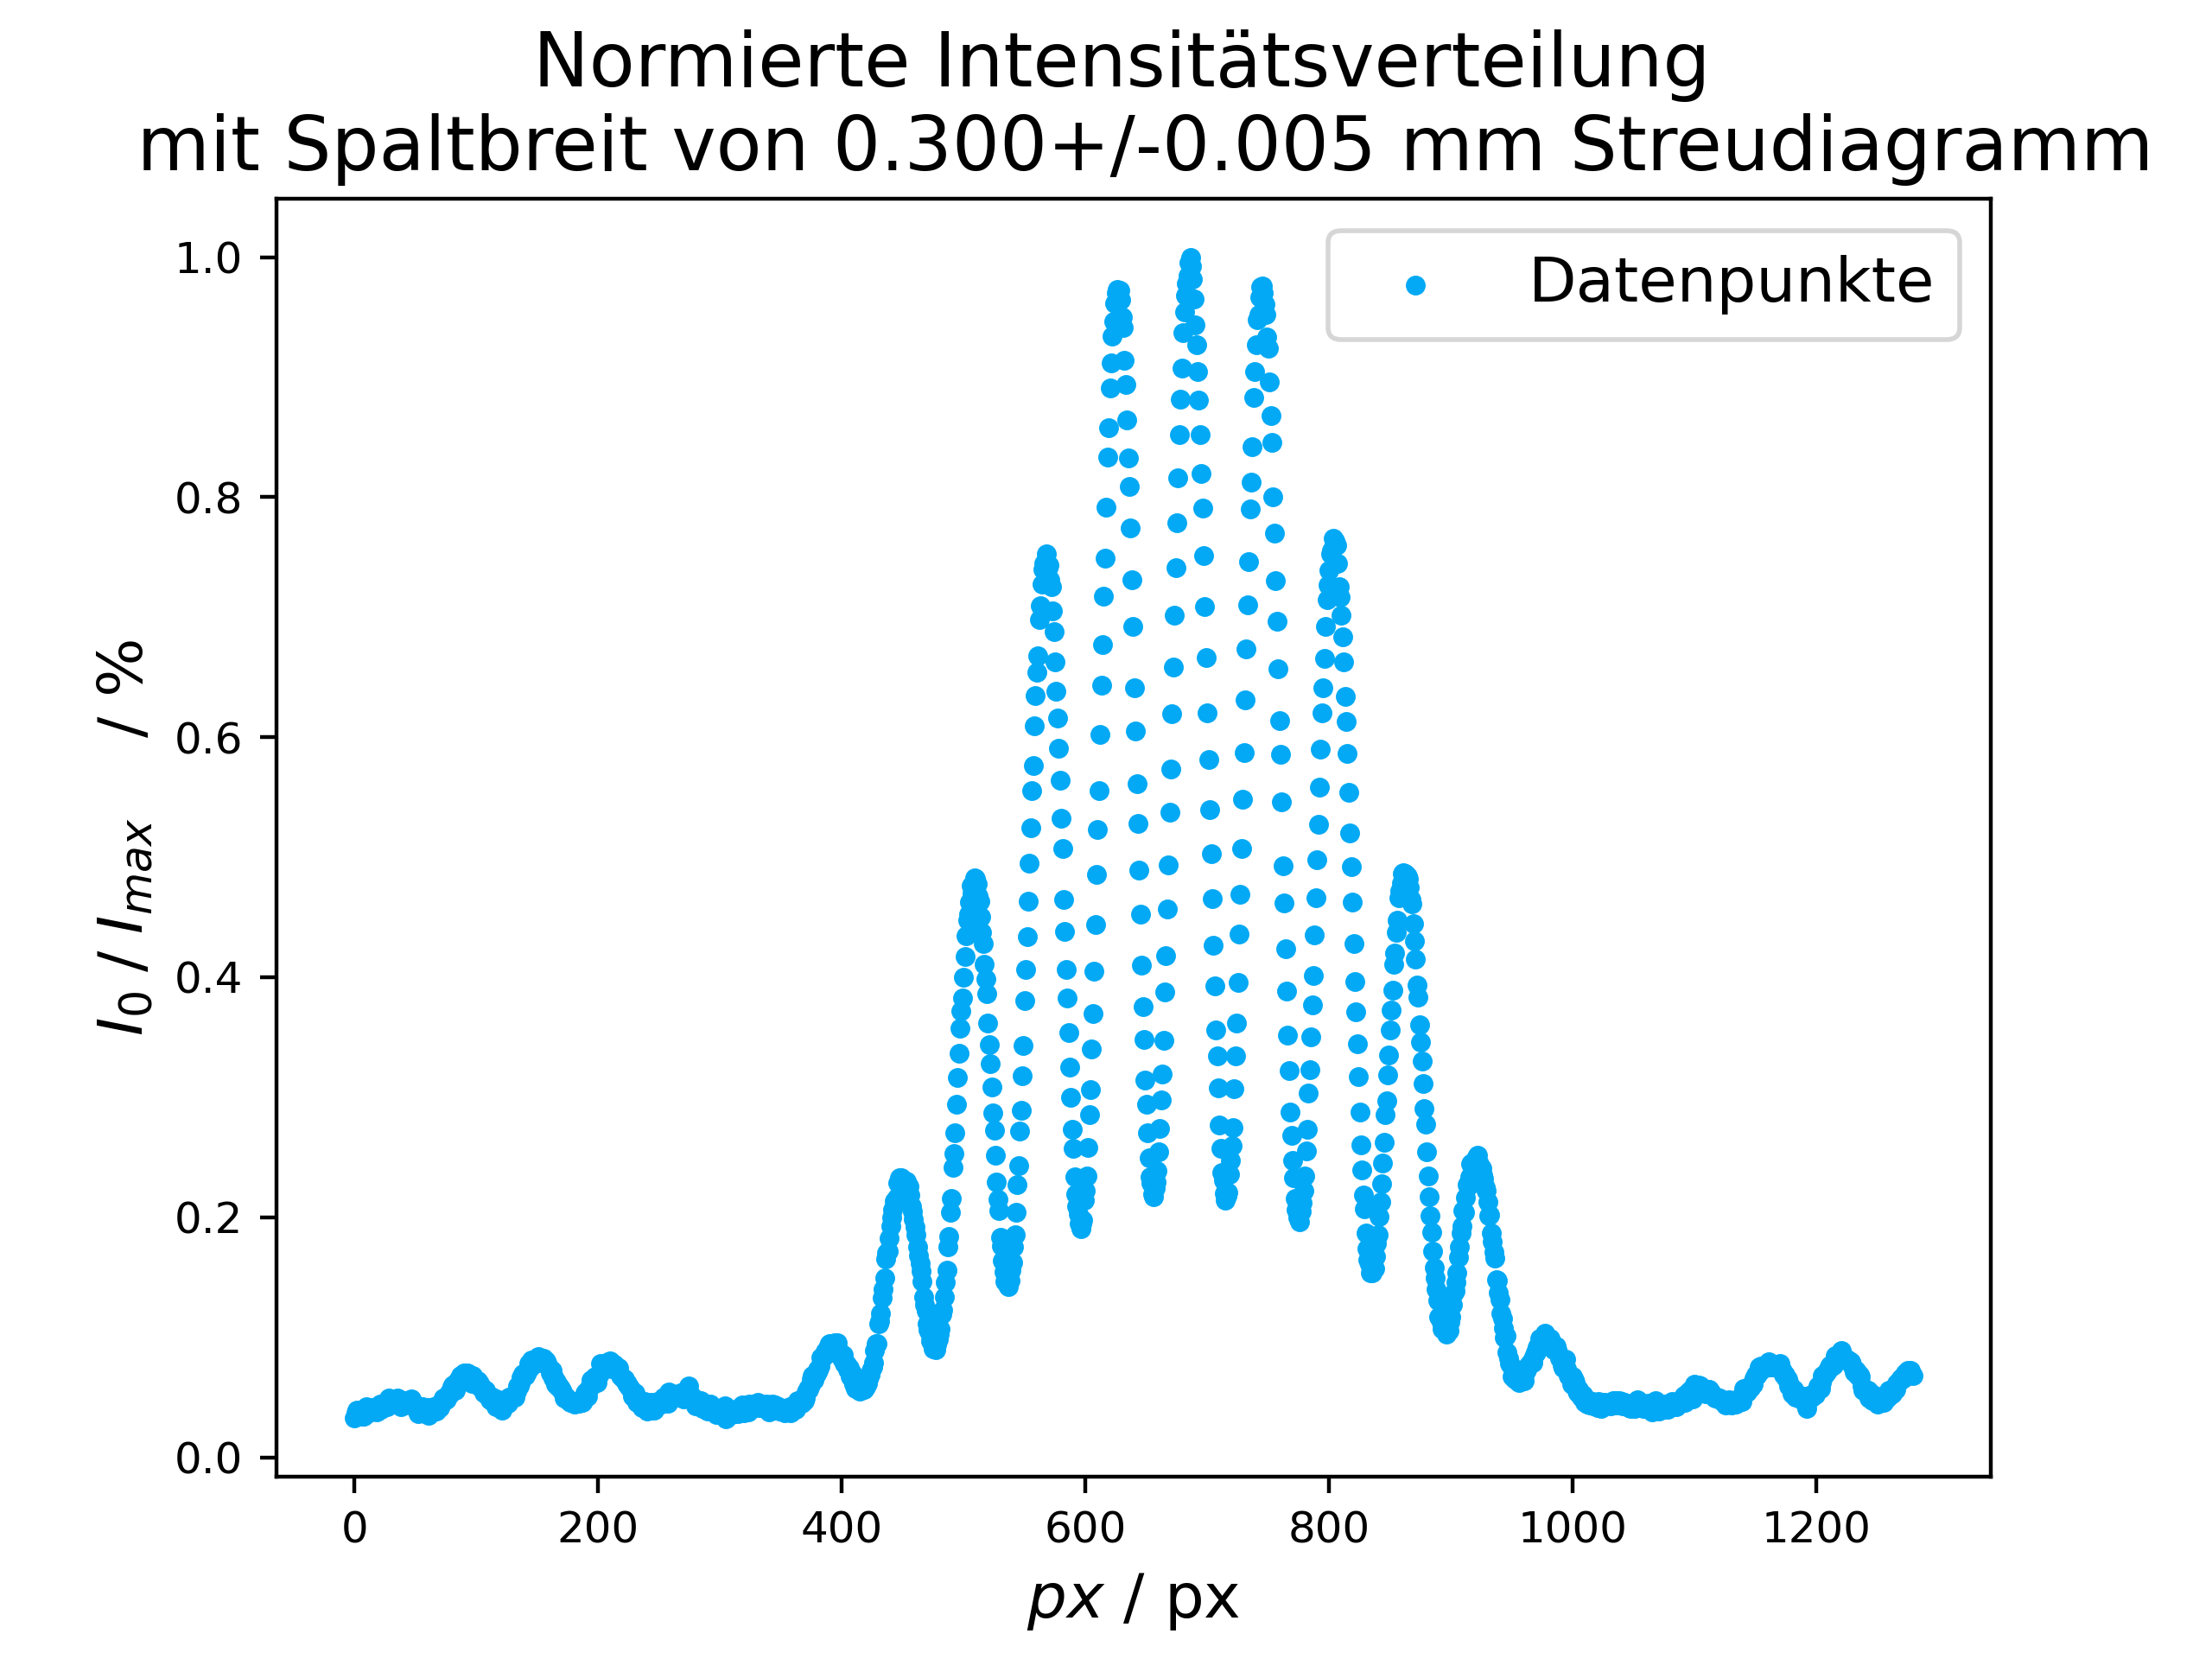
\includegraphics[width=\textwidth]{auswertung/0_09konstrast}
		\captionbelowof{figure}{geplotteter Grauwert \\ aufgetragen zu jeweiligen Pixelnummer \\ bei einer Spaltbreite von \SI{0.300(5)}{mm}}
	\end{minipage}
	\vspace{2mm}
	\begin{minipage}[t]{0.50\textwidth}
		\centering
		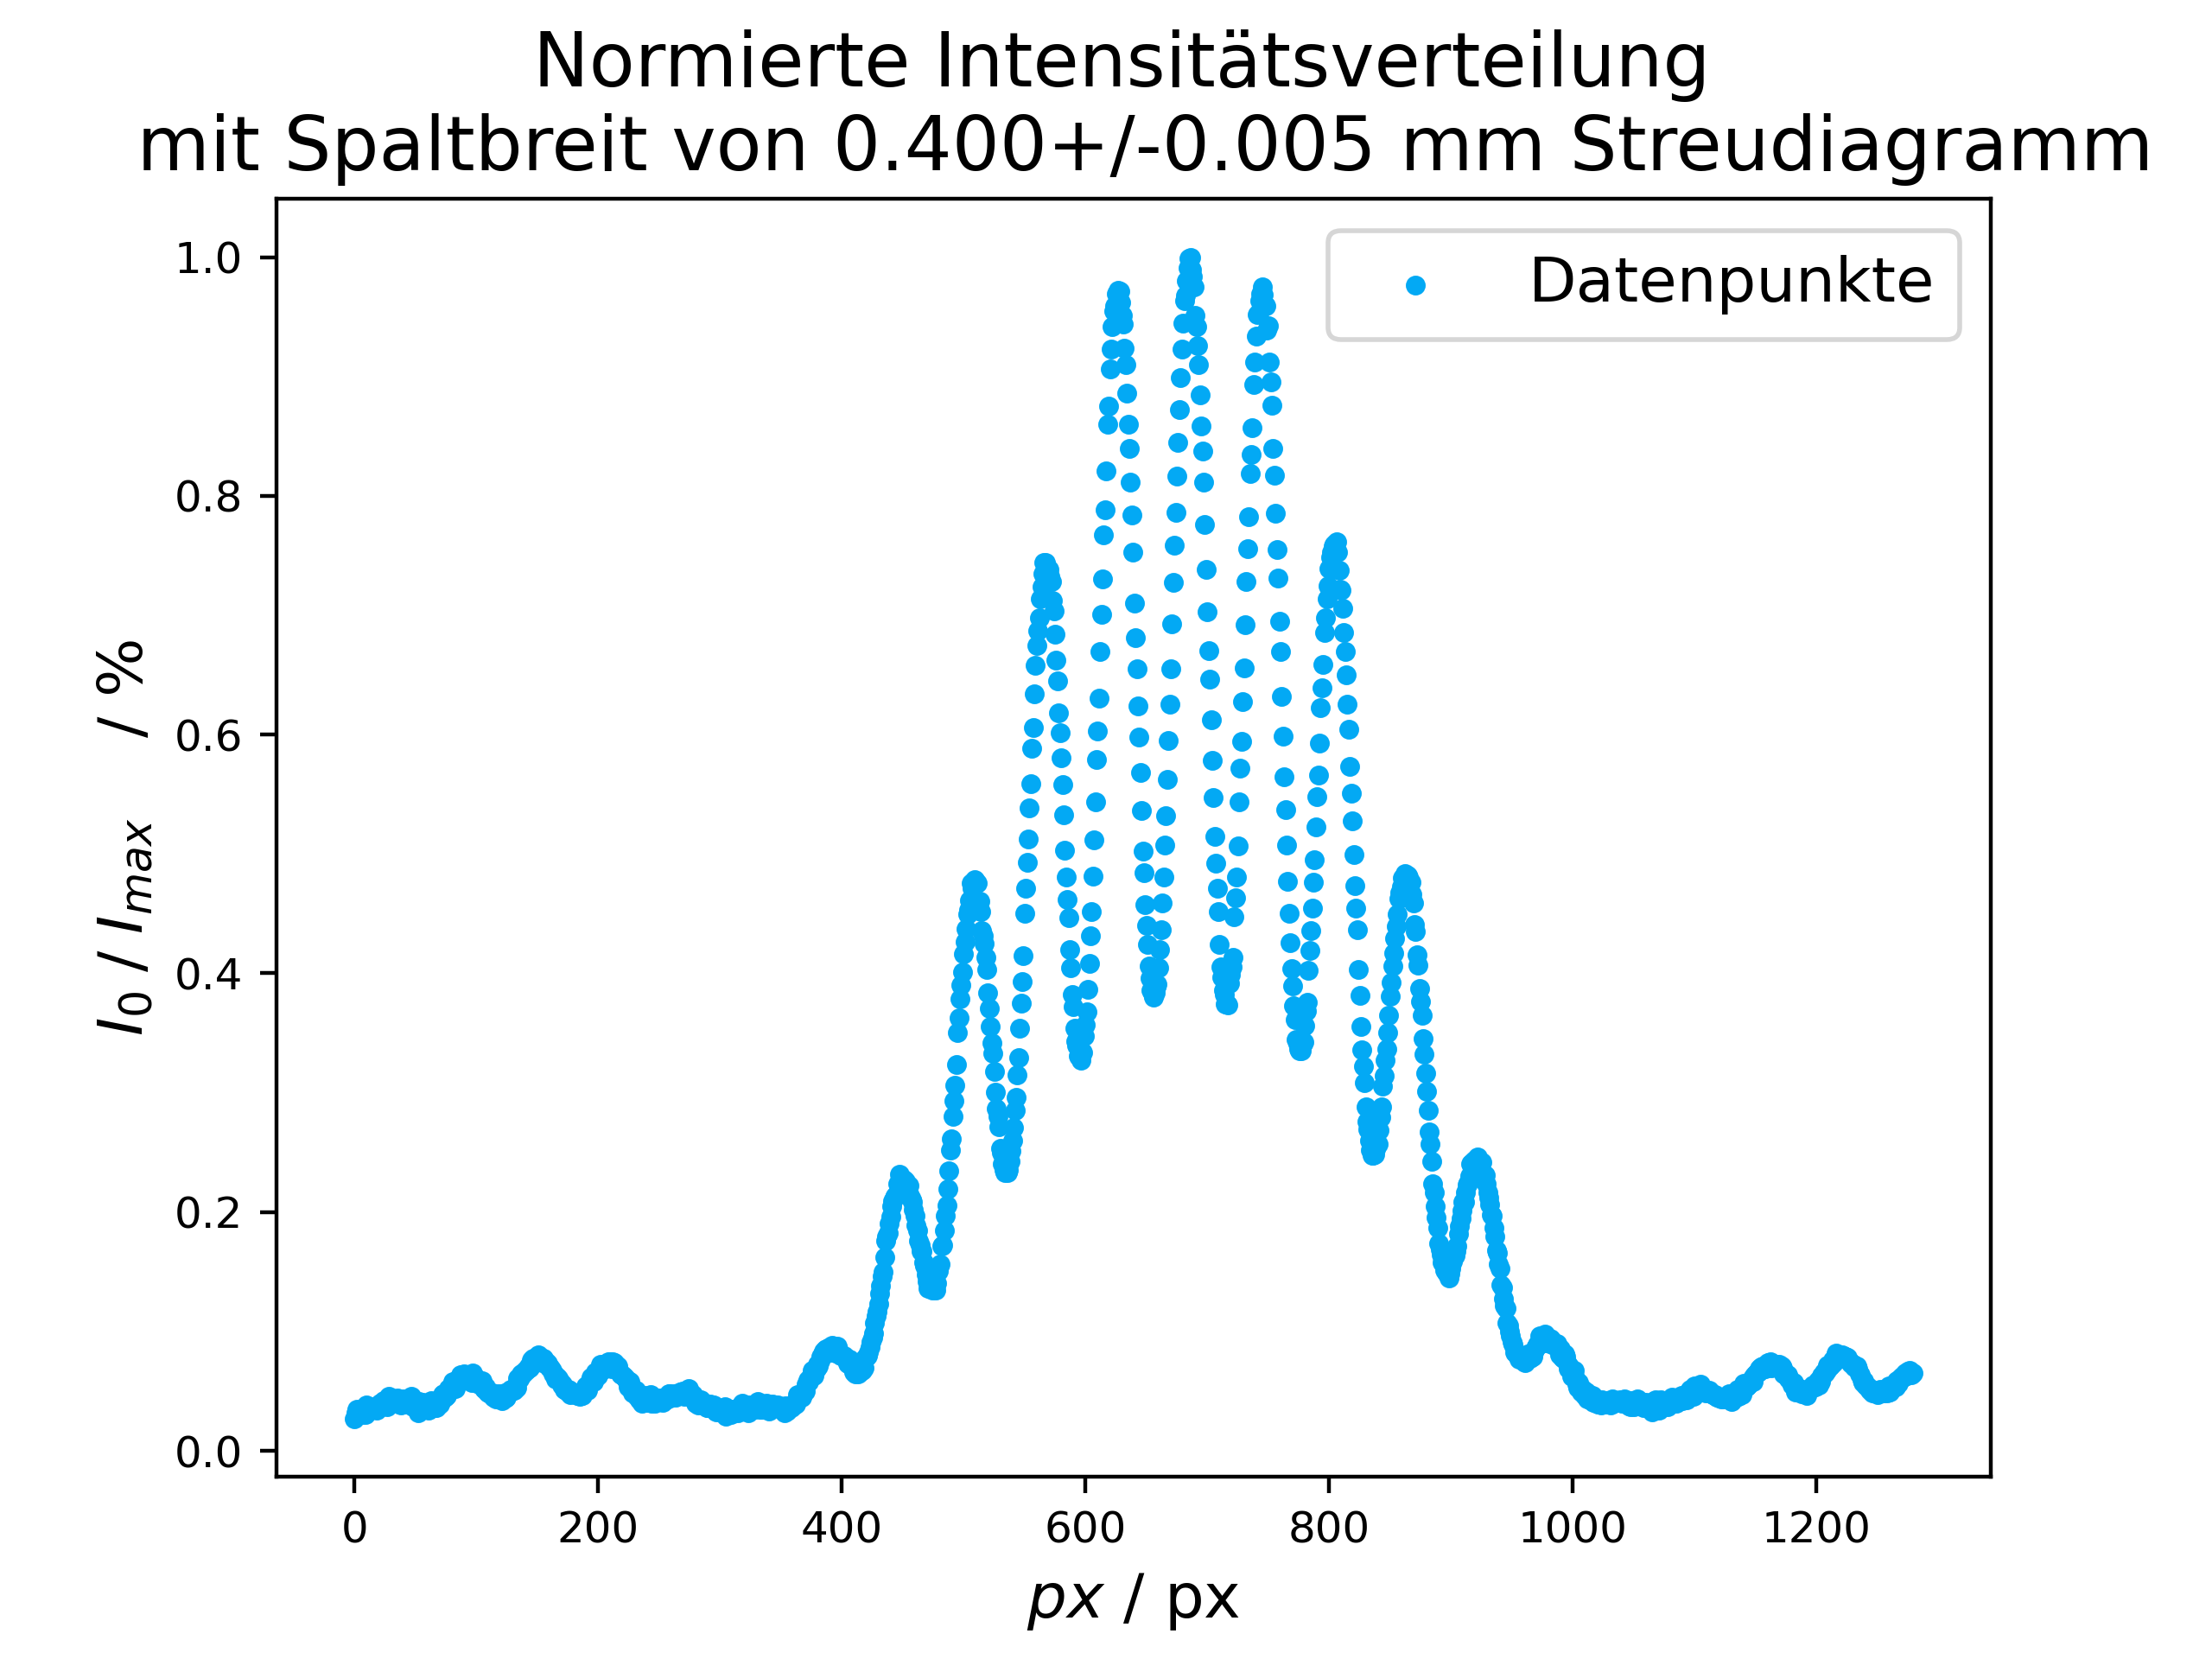
\includegraphics[width=\textwidth]{auswertung/0_19konstrast}
		\captionof{figure}{geplotteter Grauwert \\ aufgetragen zu jeweiligen Pixelnummer \\ bei einer Spaltbreite von \SI{0.400(5)}{mm}}
	\end{minipage}
	\vspace{1em}
\end{minipage}

\begin{minipage}{\textwidth}
	\begin{minipage}[t]{0.5\textwidth}
		\centering
		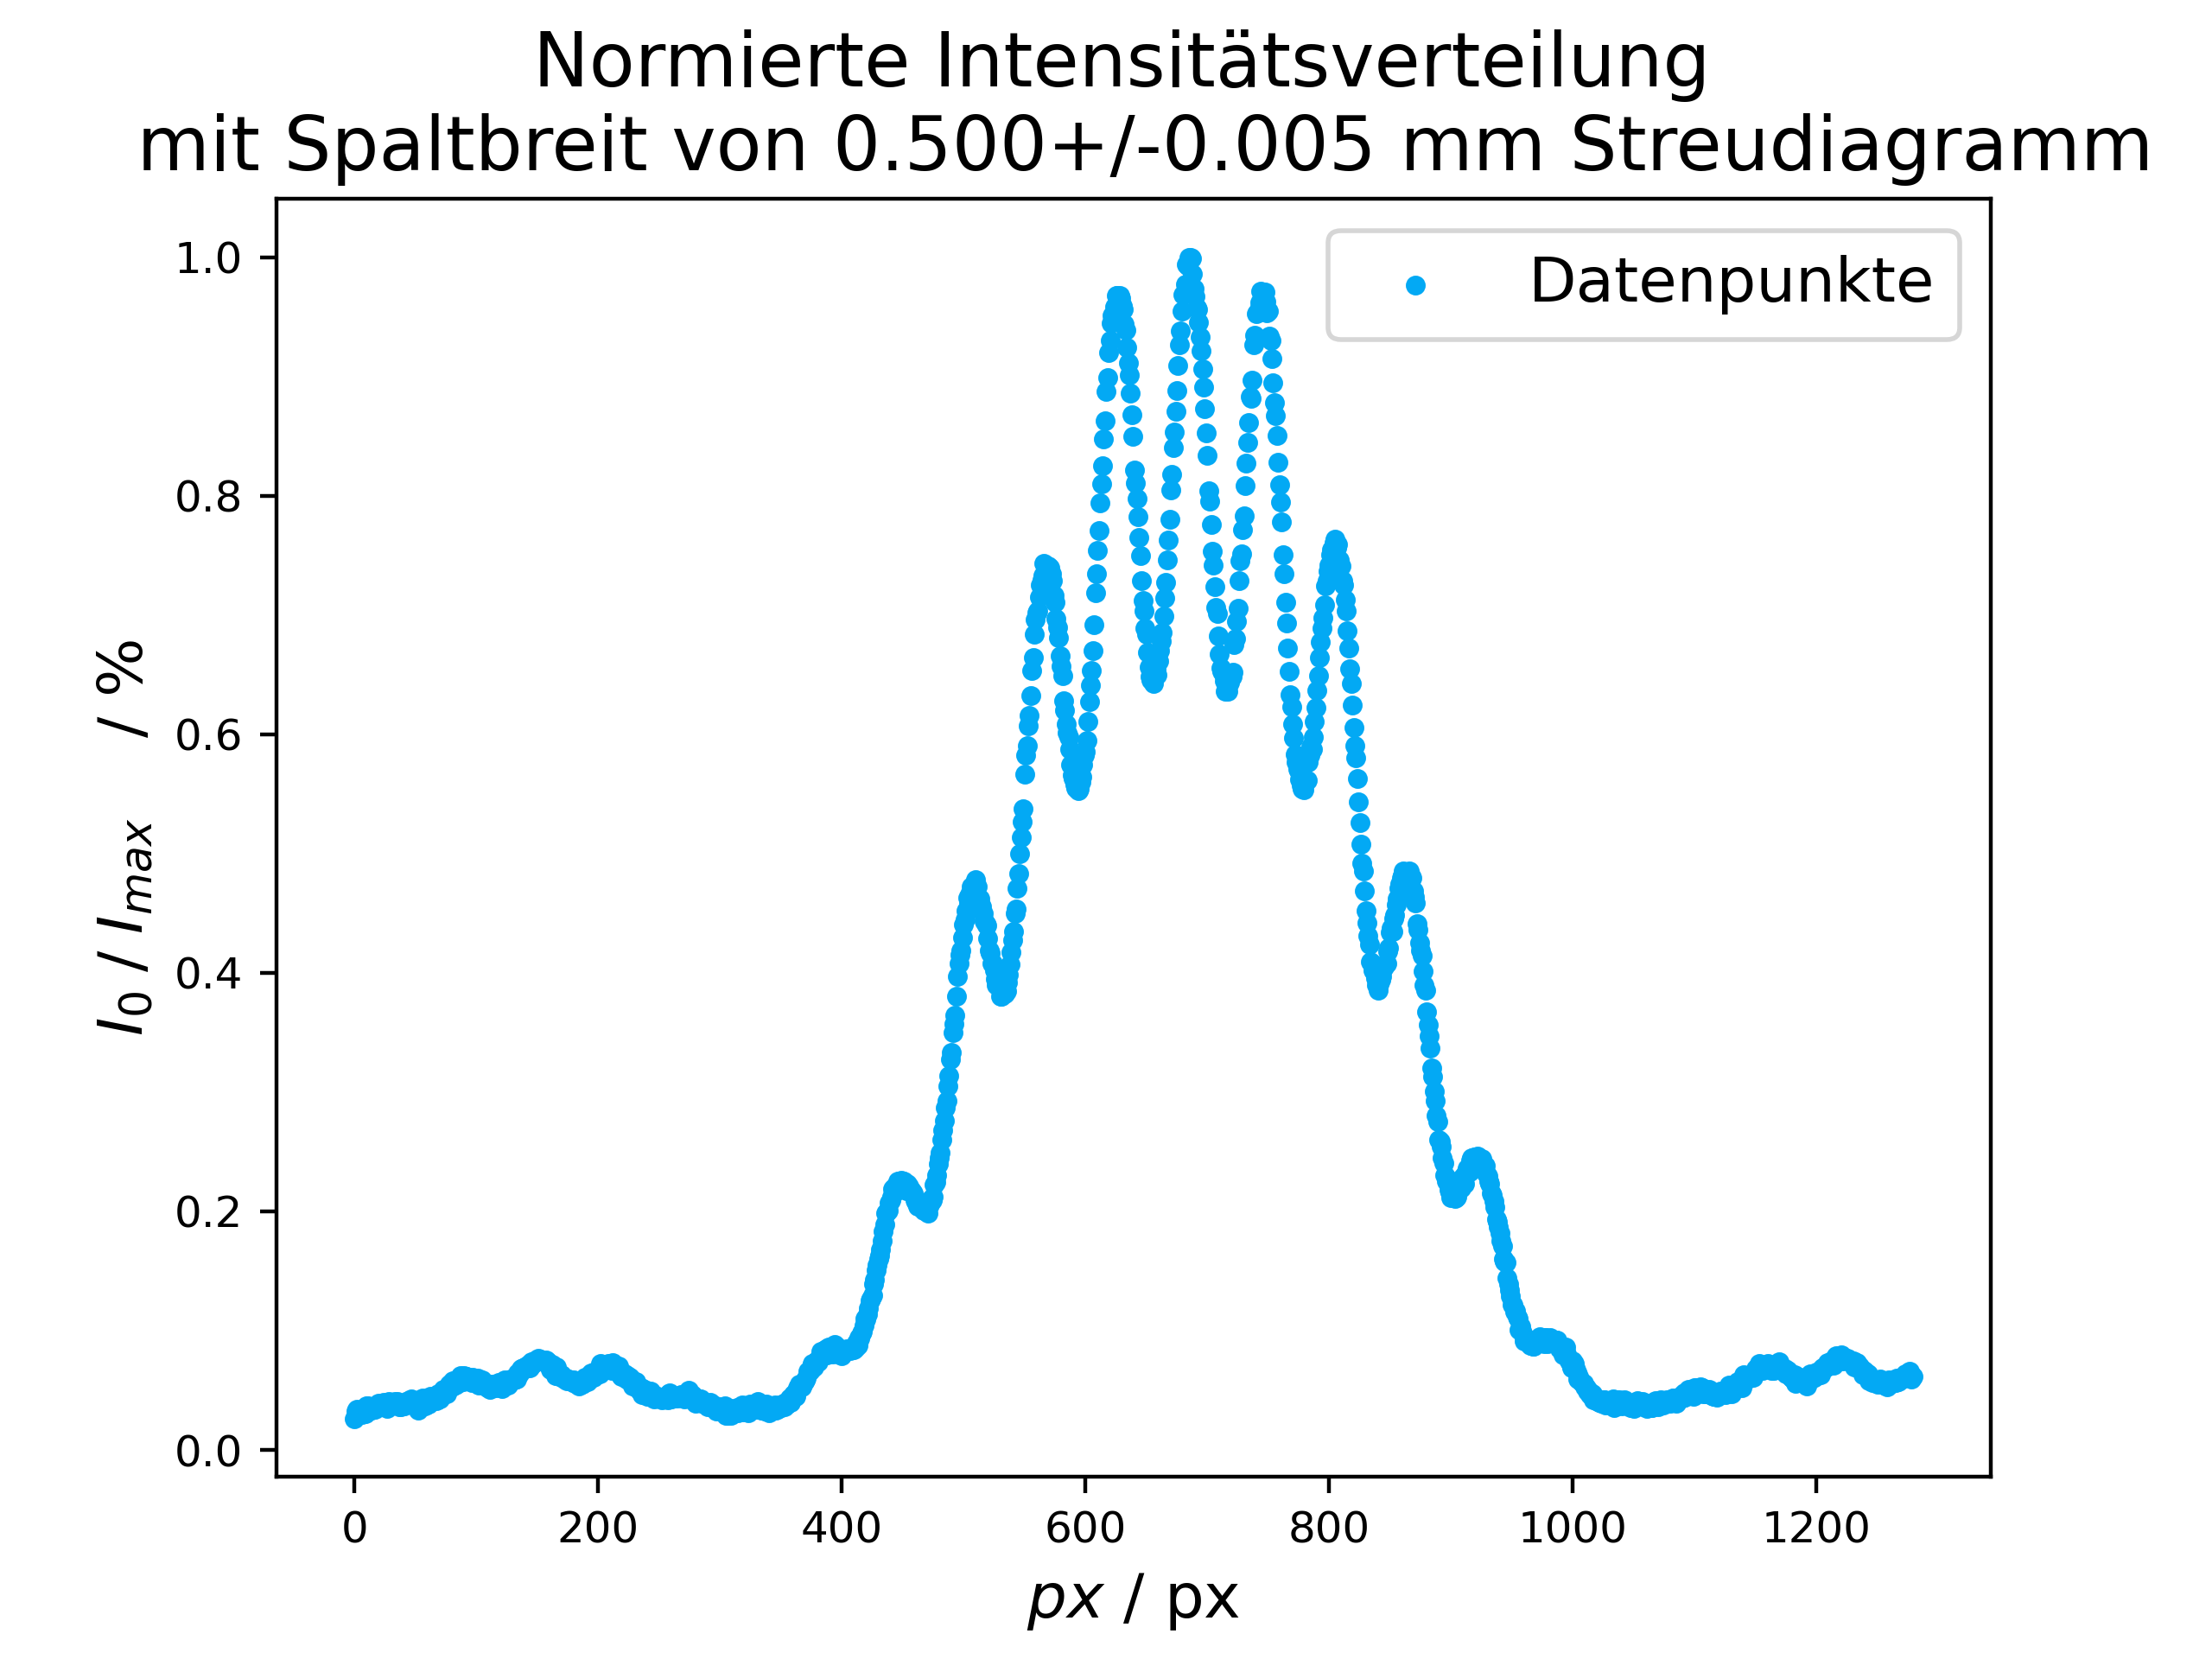
\includegraphics[width=\textwidth]{auswertung/0_29konstrast}
		\captionbelowof{figure}{geplotteter Grauwert \\ aufgetragen zu jeweiligen Pixelnummer \\ bei einer Spaltbreite von \SI{0.500(5)}{mm}}
	\end{minipage}
	\vspace{2mm}
	\begin{minipage}[t]{0.50\textwidth}
		\centering
		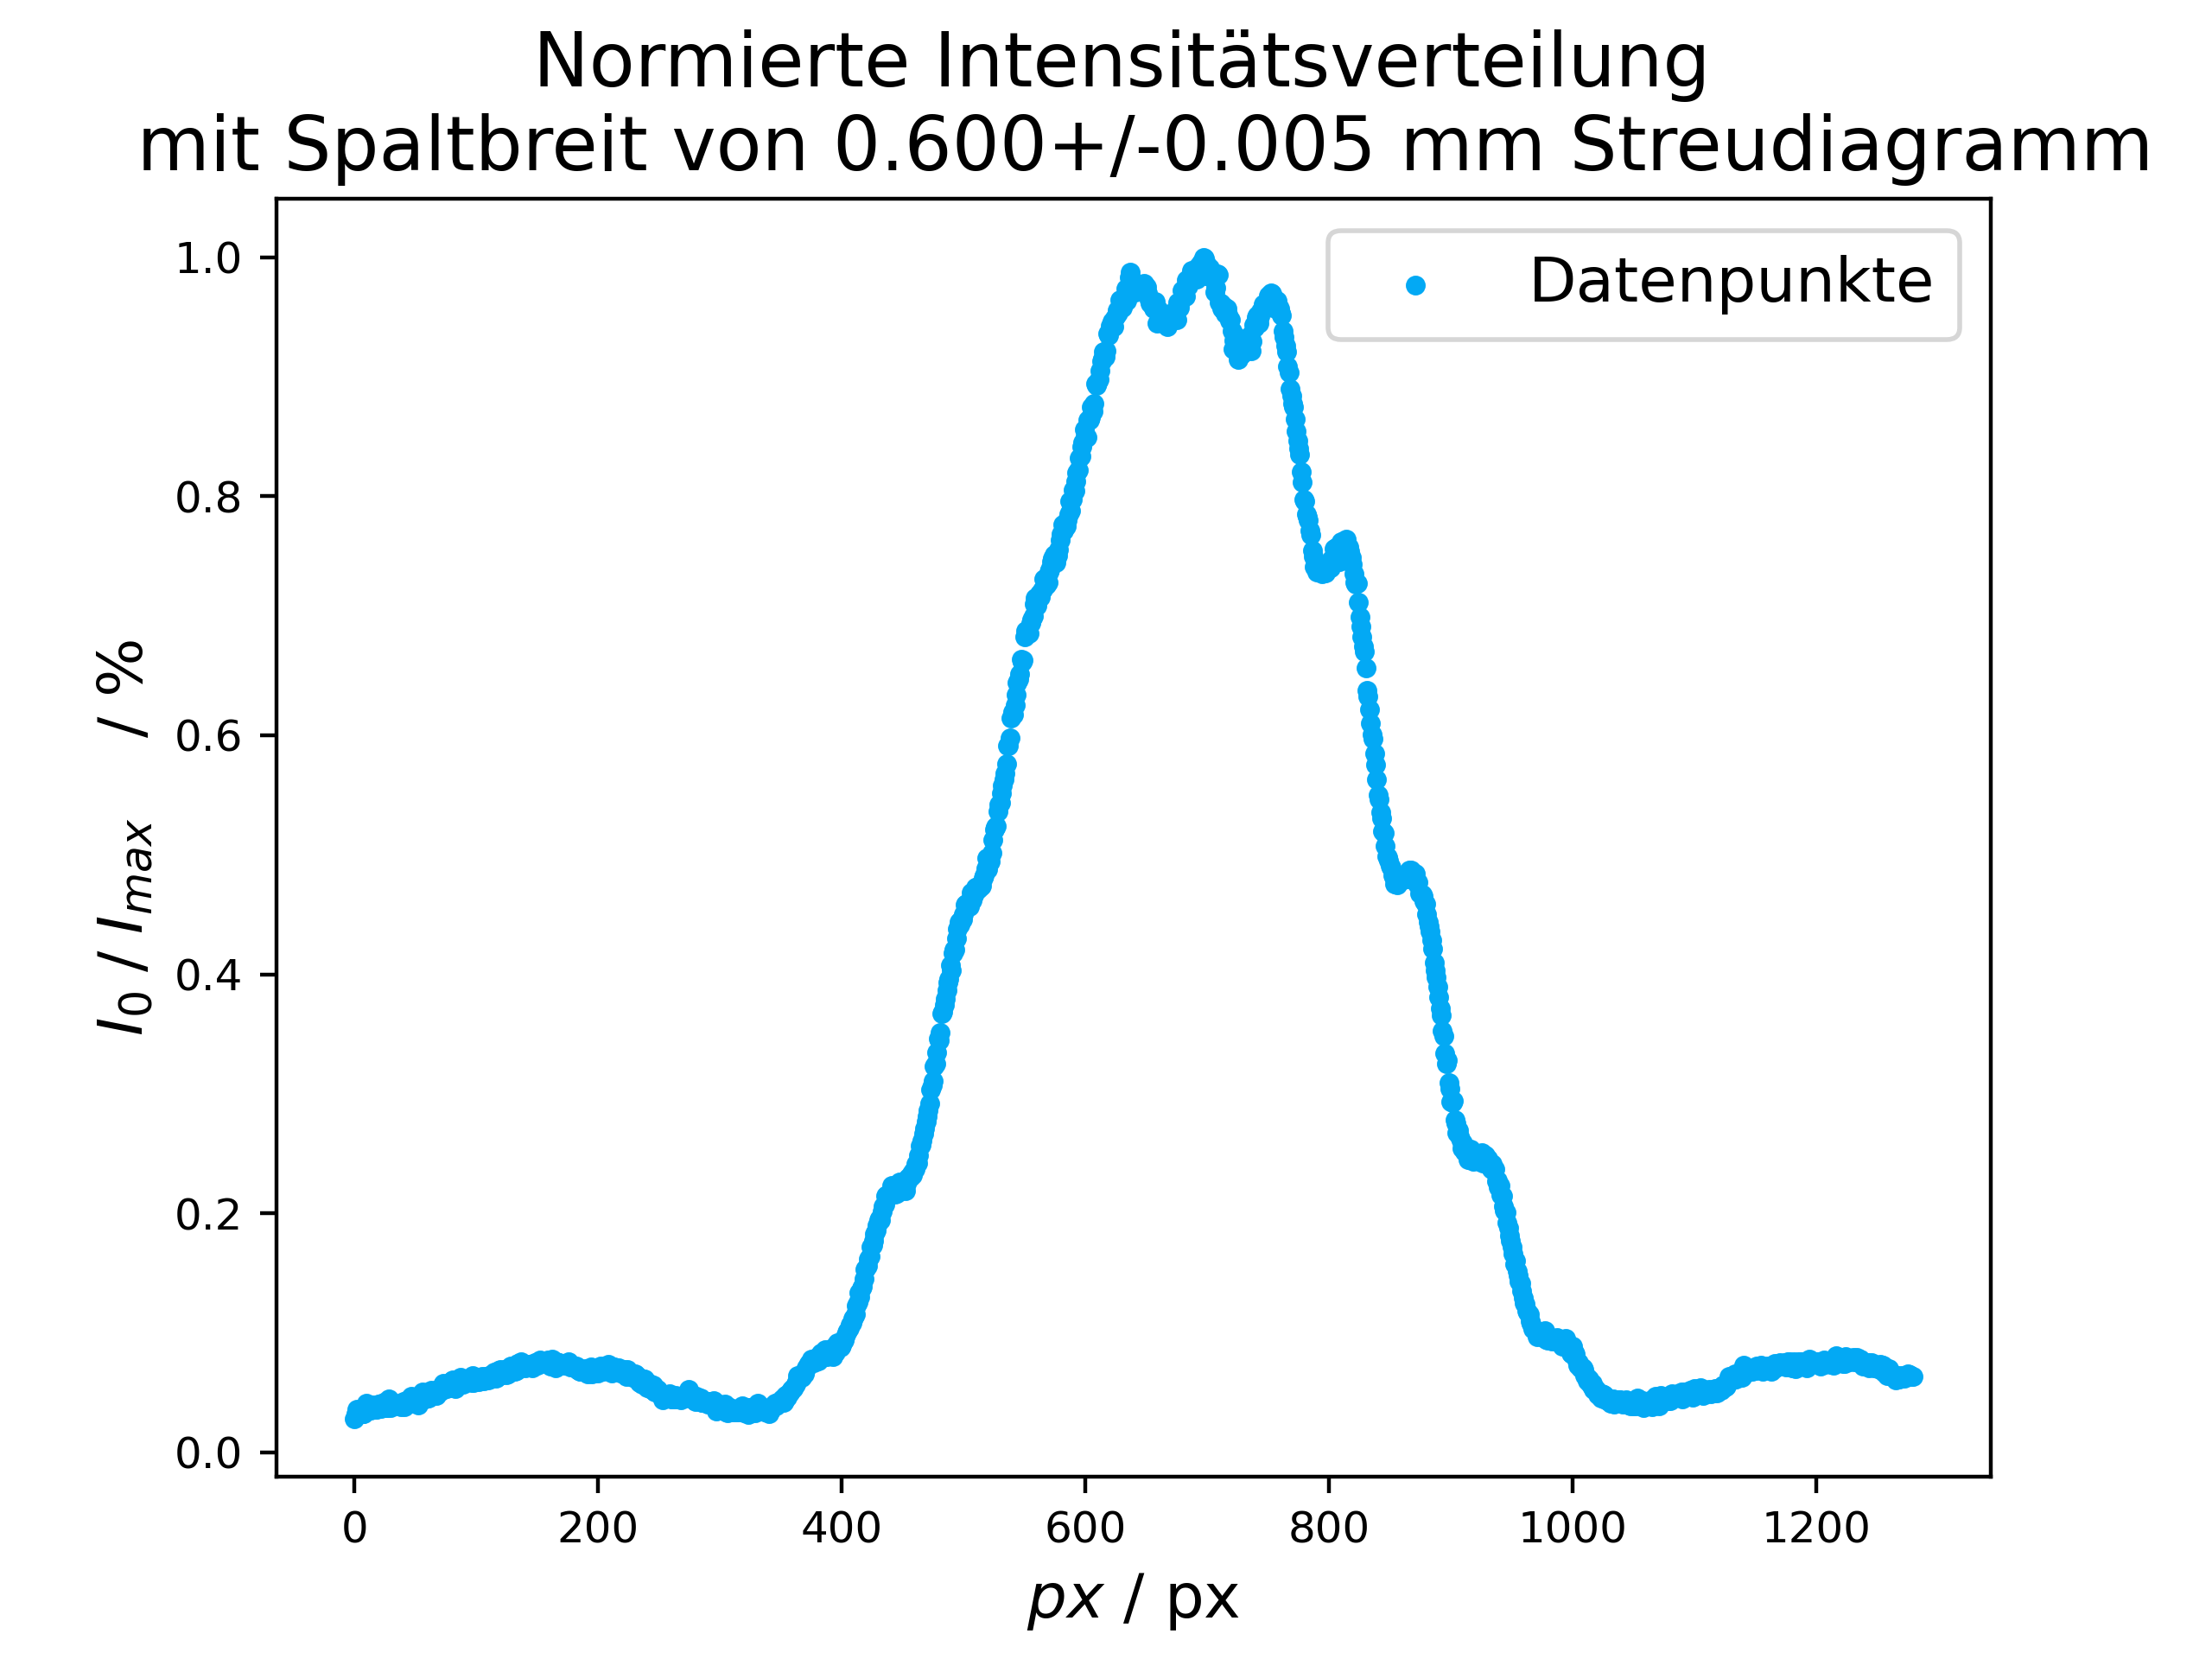
\includegraphics[width=\textwidth]{auswertung/0_39konstrast}
		\captionof{figure}{geplotteter Grauwert \\ aufgetragen zu jeweiligen Pixelnummer \\ bei einer Spaltbreite von \SI{0.600(5)}{mm}}
	\end{minipage}
	\vspace{1em}
\end{minipage}

\begin{minipage}{\textwidth}
	\begin{minipage}[t]{0.5\textwidth}
		\centering
		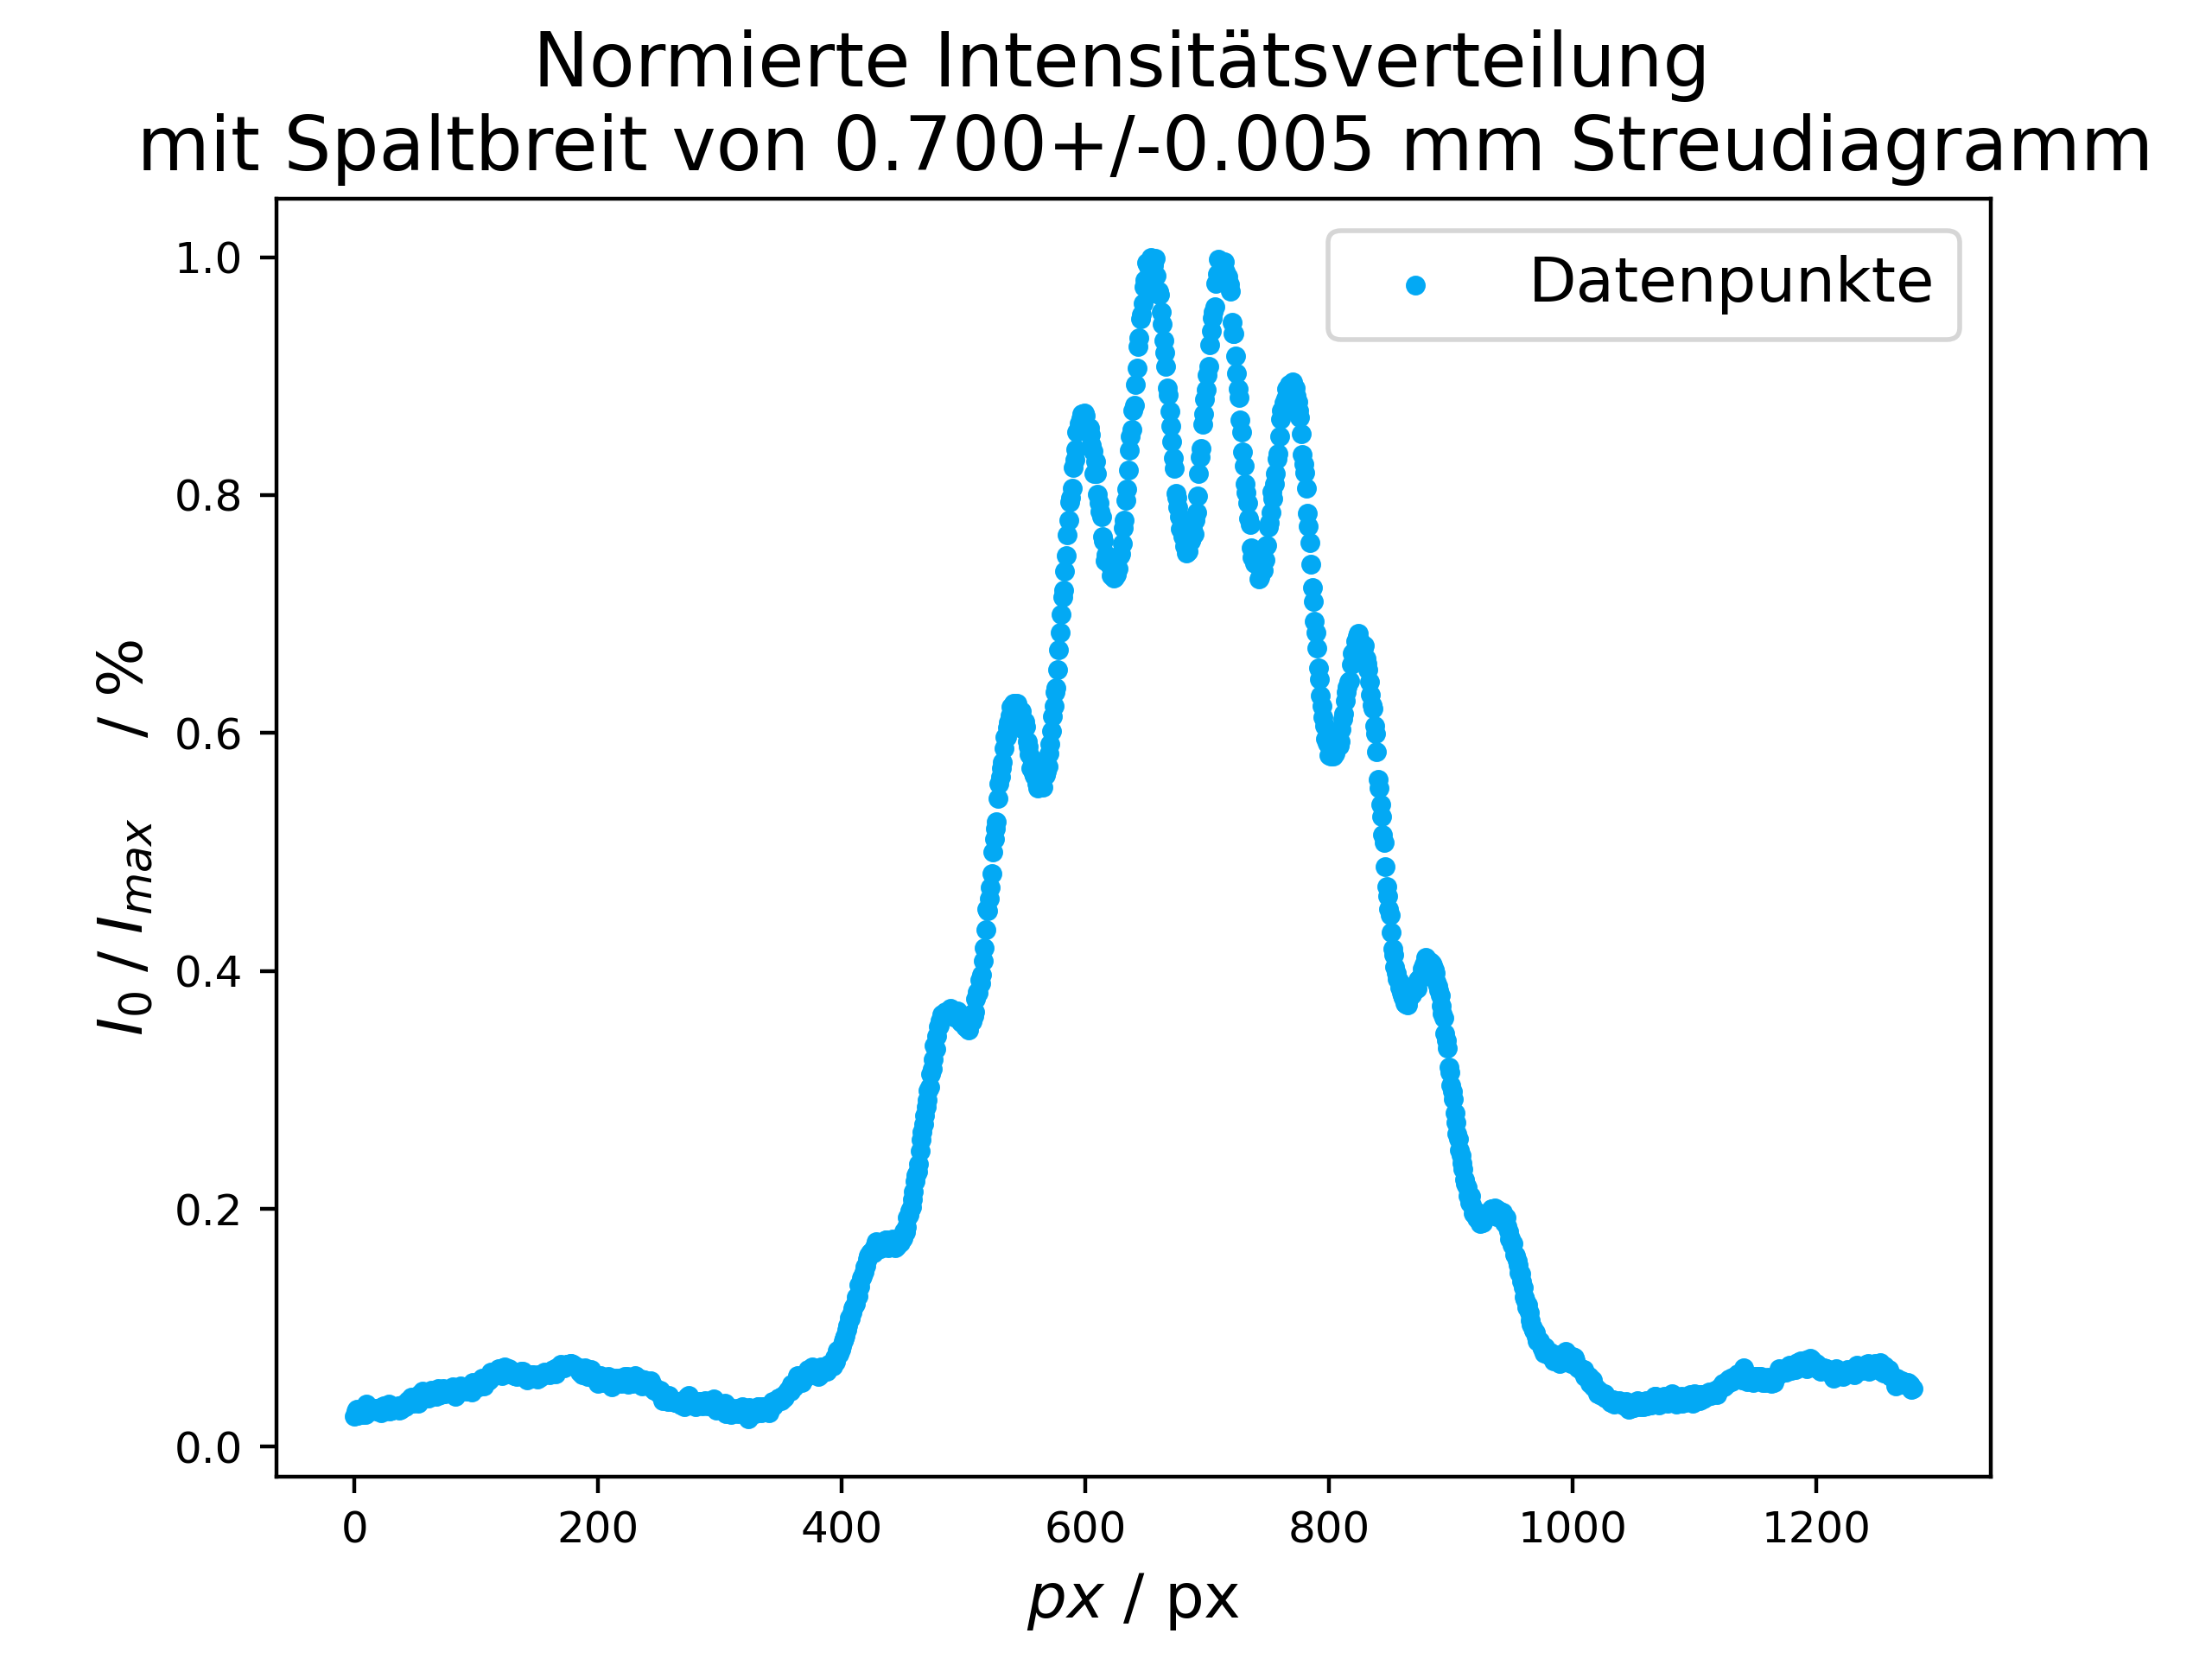
\includegraphics[width=\textwidth]{auswertung/0_49konstrast}
		\captionbelowof{figure}{geplotteter Grauwert \\ aufgetragen zu jeweiligen Pixelnummer \\ bei einer Spaltbreite von \SI{0.700(5)}{mm}}
	\end{minipage}
	\vspace{2mm}
	\begin{minipage}[t]{0.50\textwidth}
		\centering
		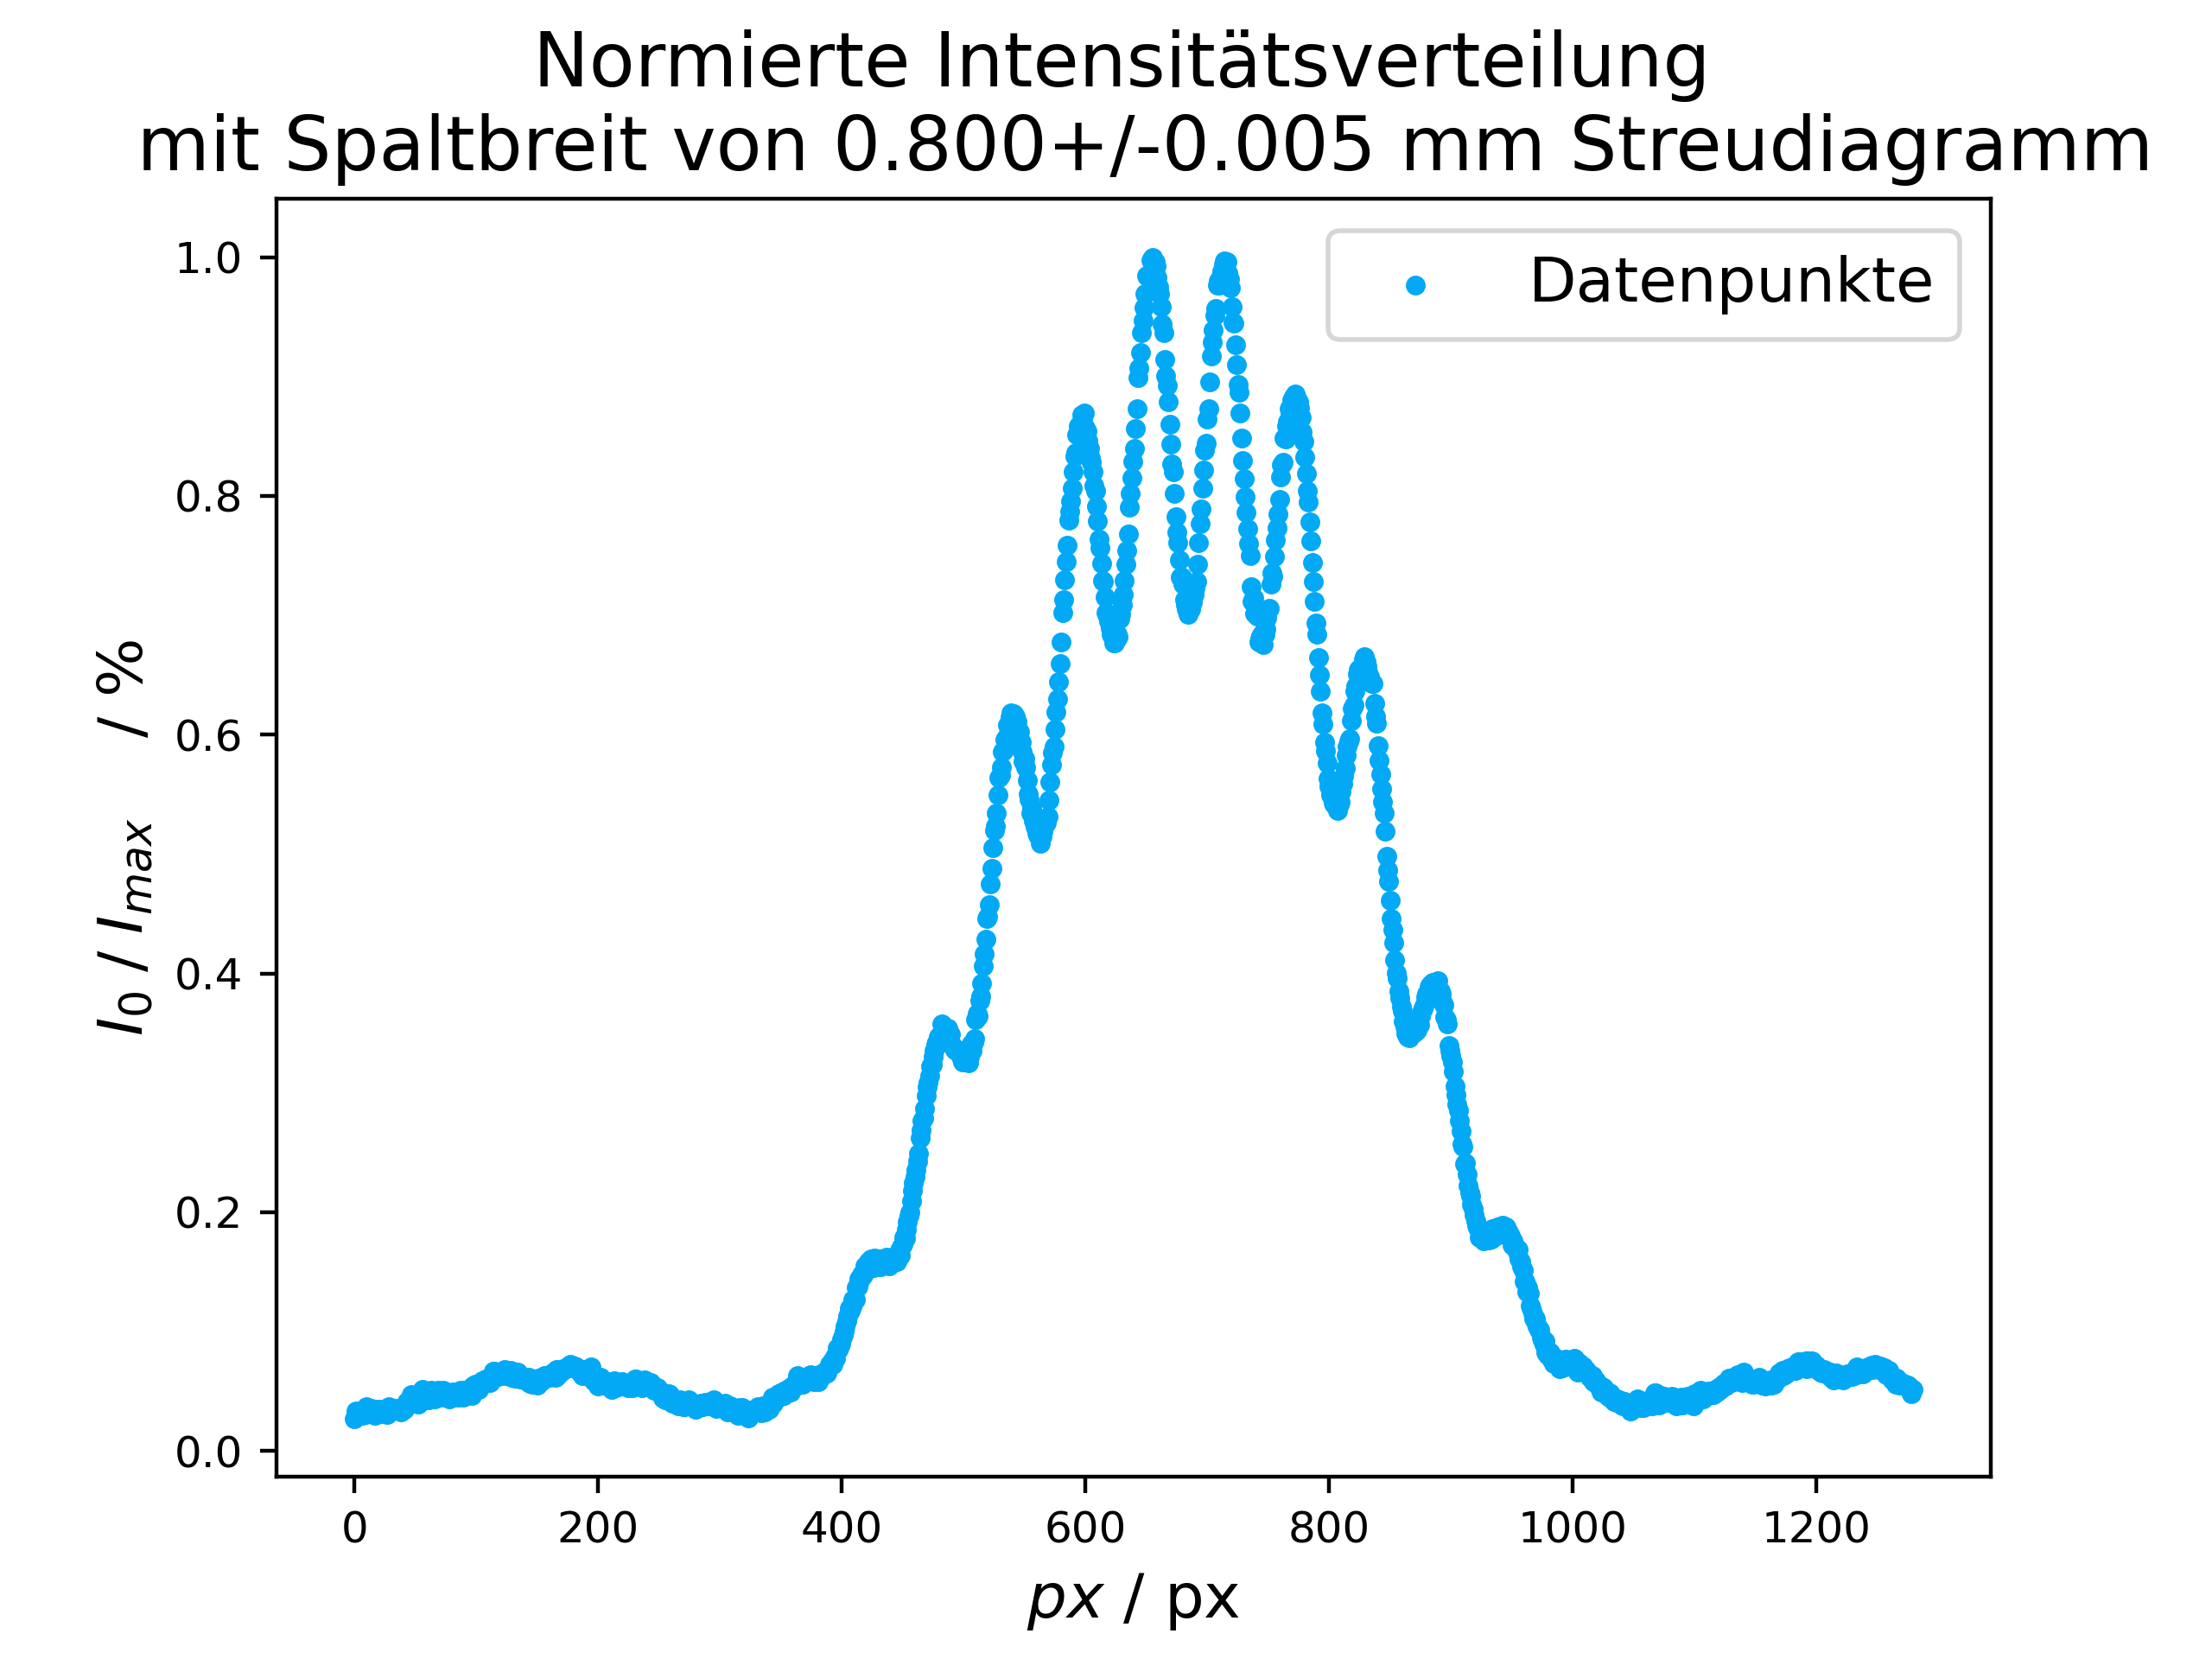
\includegraphics[width=\textwidth]{auswertung/0_59konstrast}
		\captionof{figure}{geplotteter Grauwert \\ aufgetragen zu jeweiligen Pixelnummer \\ bei einer Spaltbreite von \SI{0.800(5)}{mm}}
	\end{minipage}
	\vspace{1em}
\end{minipage}

\begin{minipage}{\textwidth}
	\begin{minipage}[t]{0.5\textwidth}
		\centering
		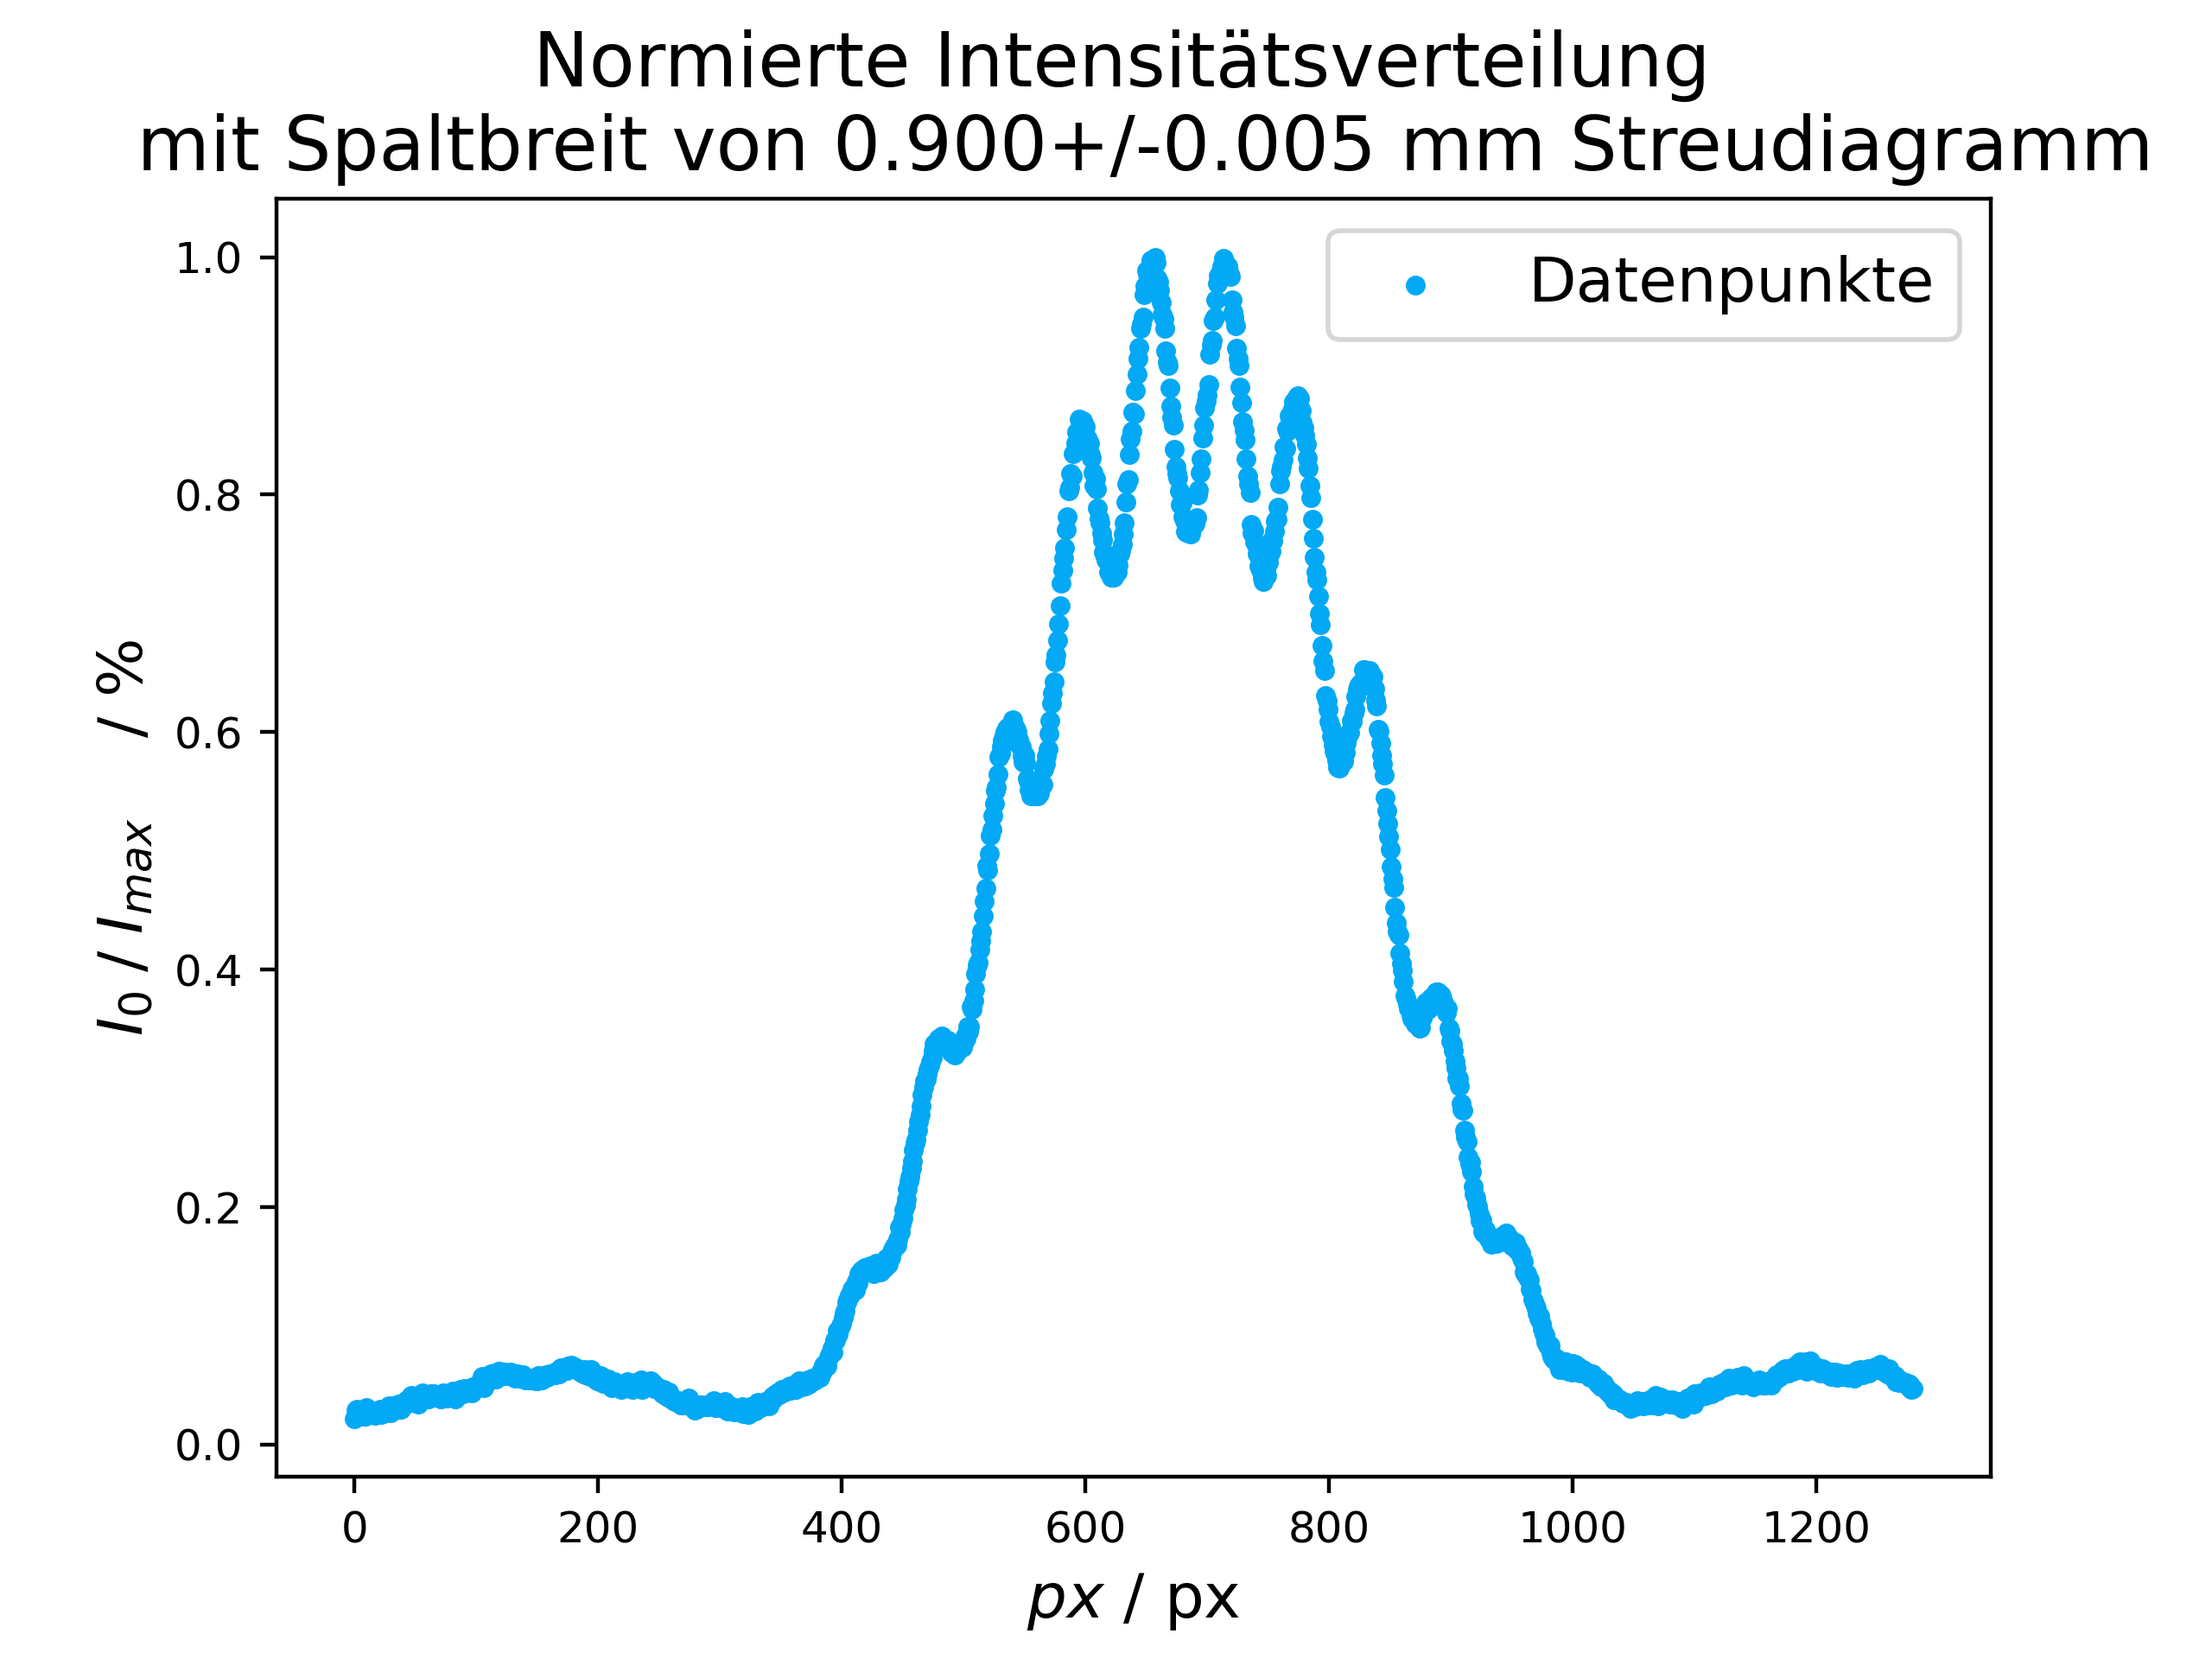
\includegraphics[width=\textwidth]{auswertung/0_69konstrast}
		\captionbelowof{figure}{geplotteter Grauwert \\ aufgetragen zu jeweiligen Pixelnummer \\ bei einer Spaltbreite von \SI{0.900(5)}{mm}}
	\end{minipage}
	\vspace{2mm}
	\begin{minipage}[t]{0.50\textwidth}
		\centering
		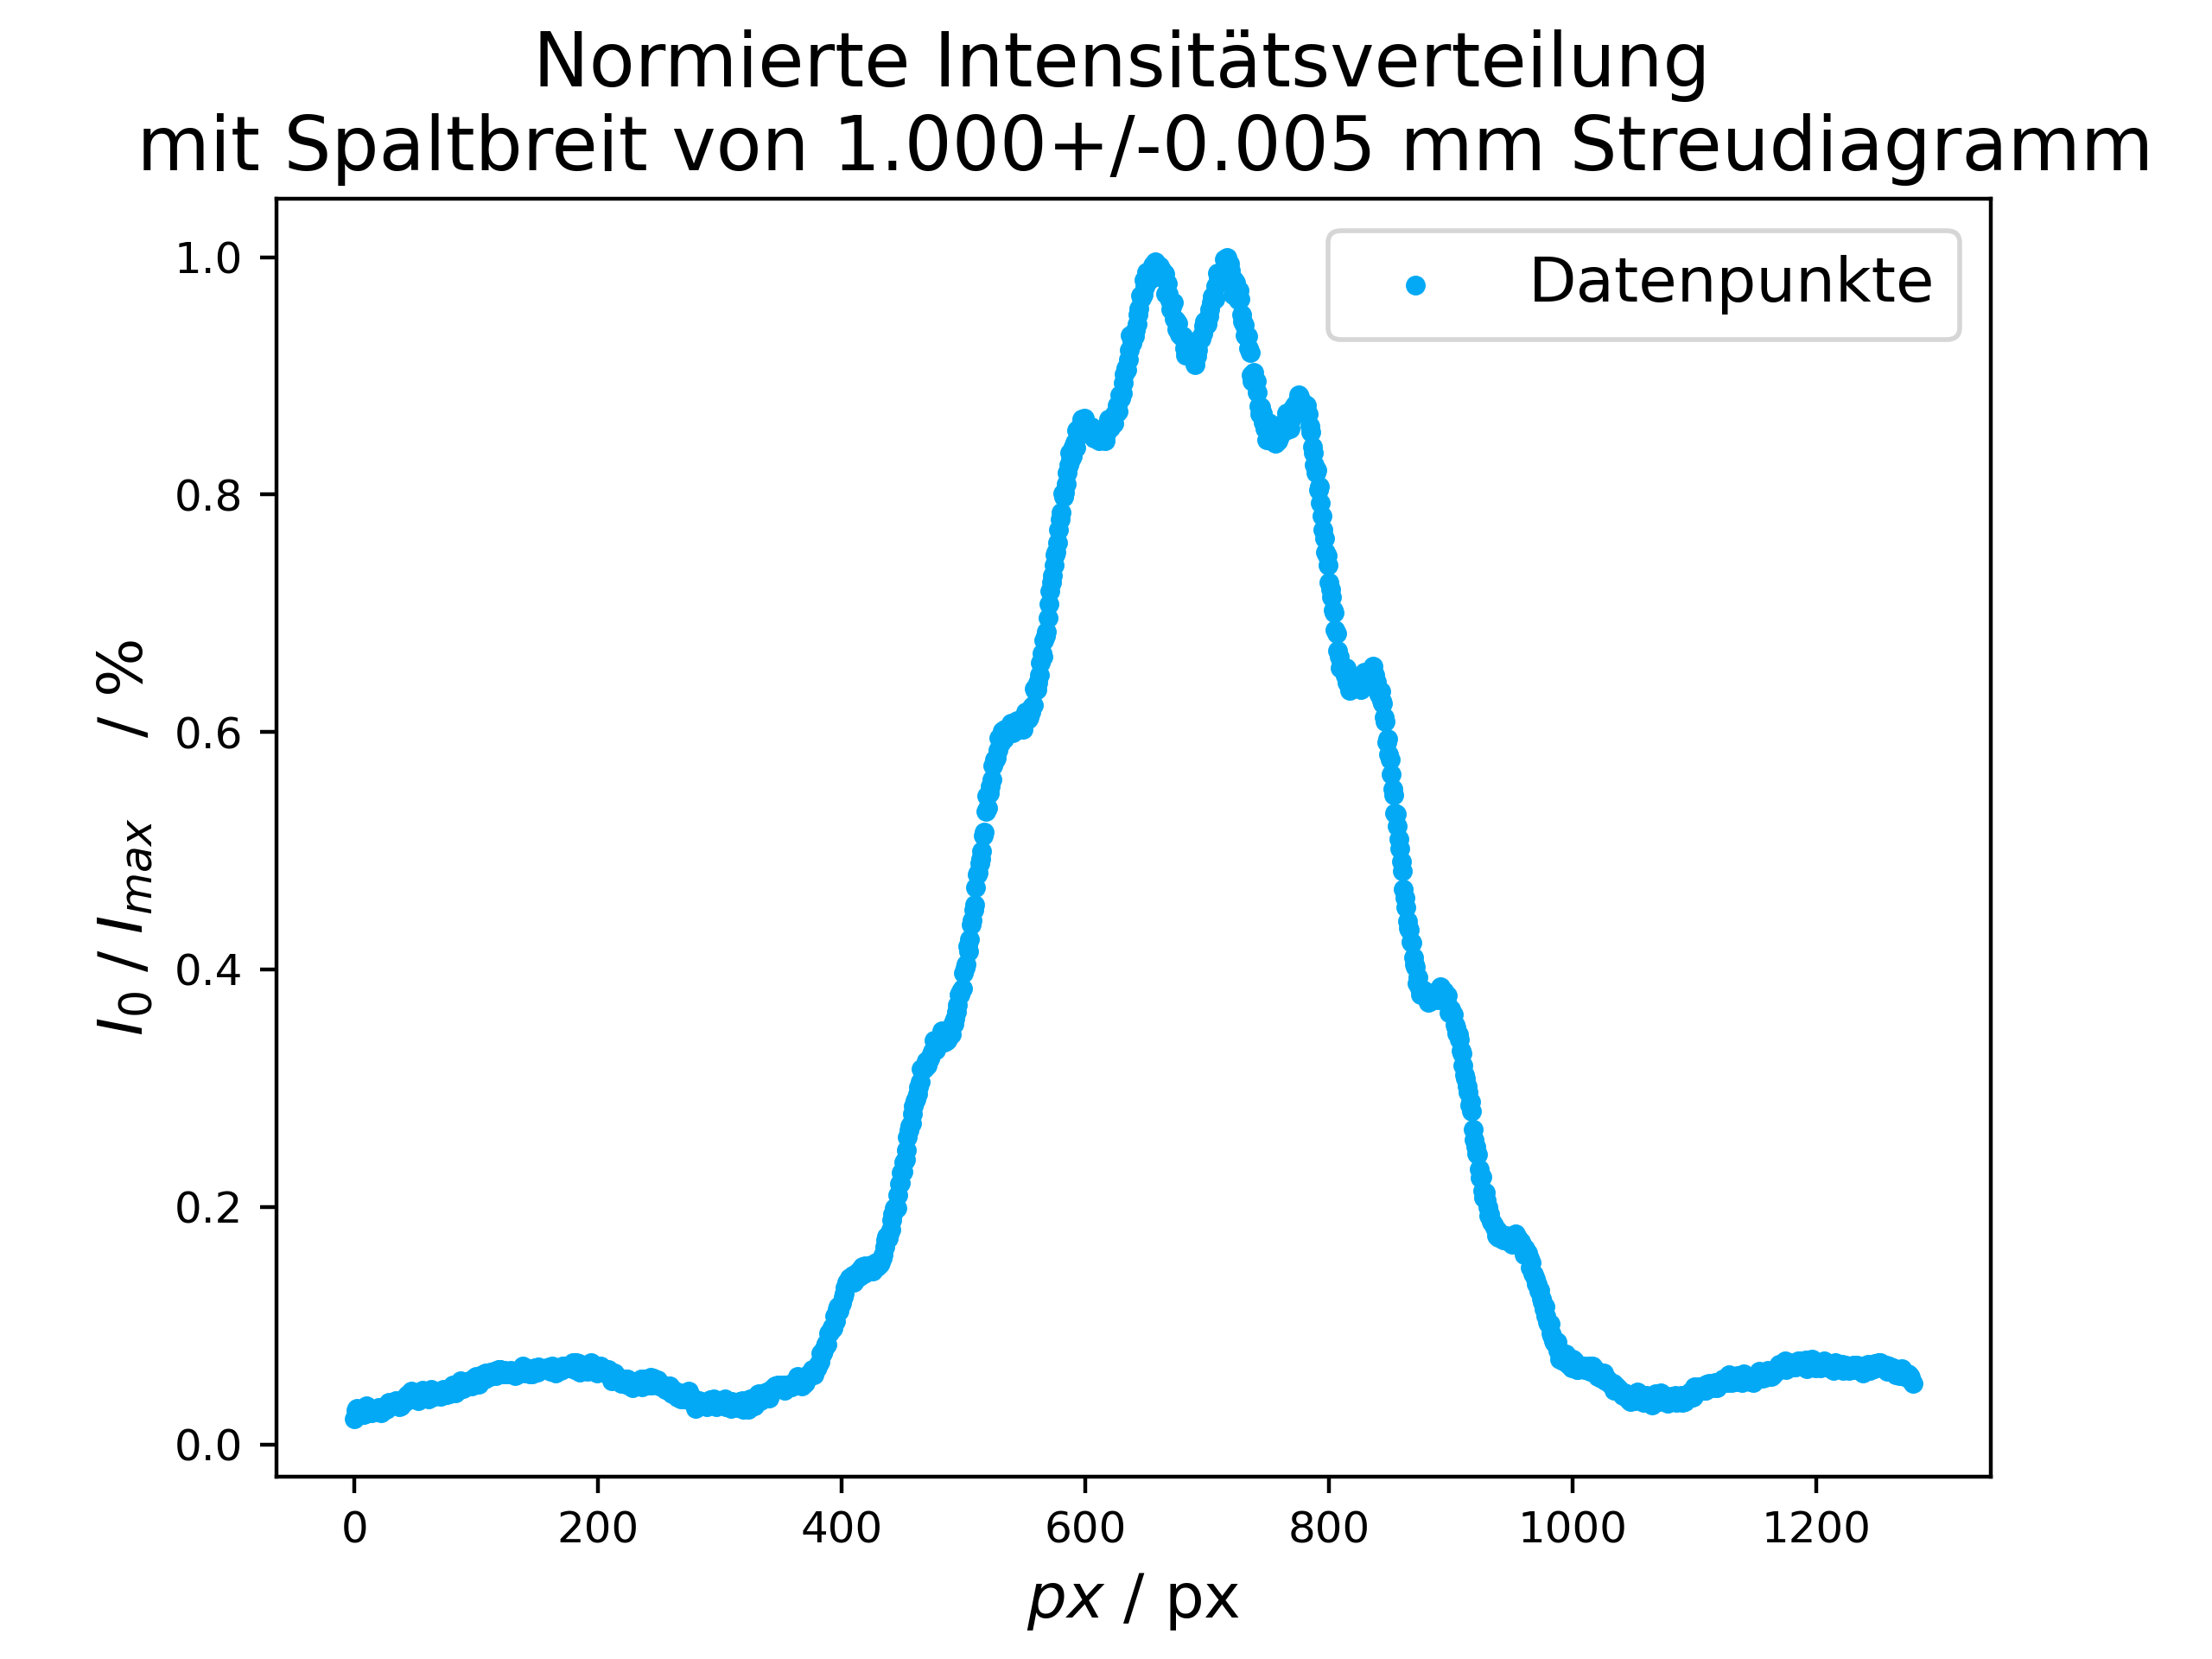
\includegraphics[width=\textwidth]{auswertung/0_79konstrast}
		\captionof{figure}{geplotteter Grauwert \\ aufgetragen zu jeweiligen Pixelnummer \\ bei einer Spaltbreite von \SI{1.000(5)}{mm}}
	\end{minipage}
	\vspace{1em}
\end{minipage}

\begin{minipage}{\textwidth}
	\begin{minipage}[t]{0.5\textwidth}
		\centering
		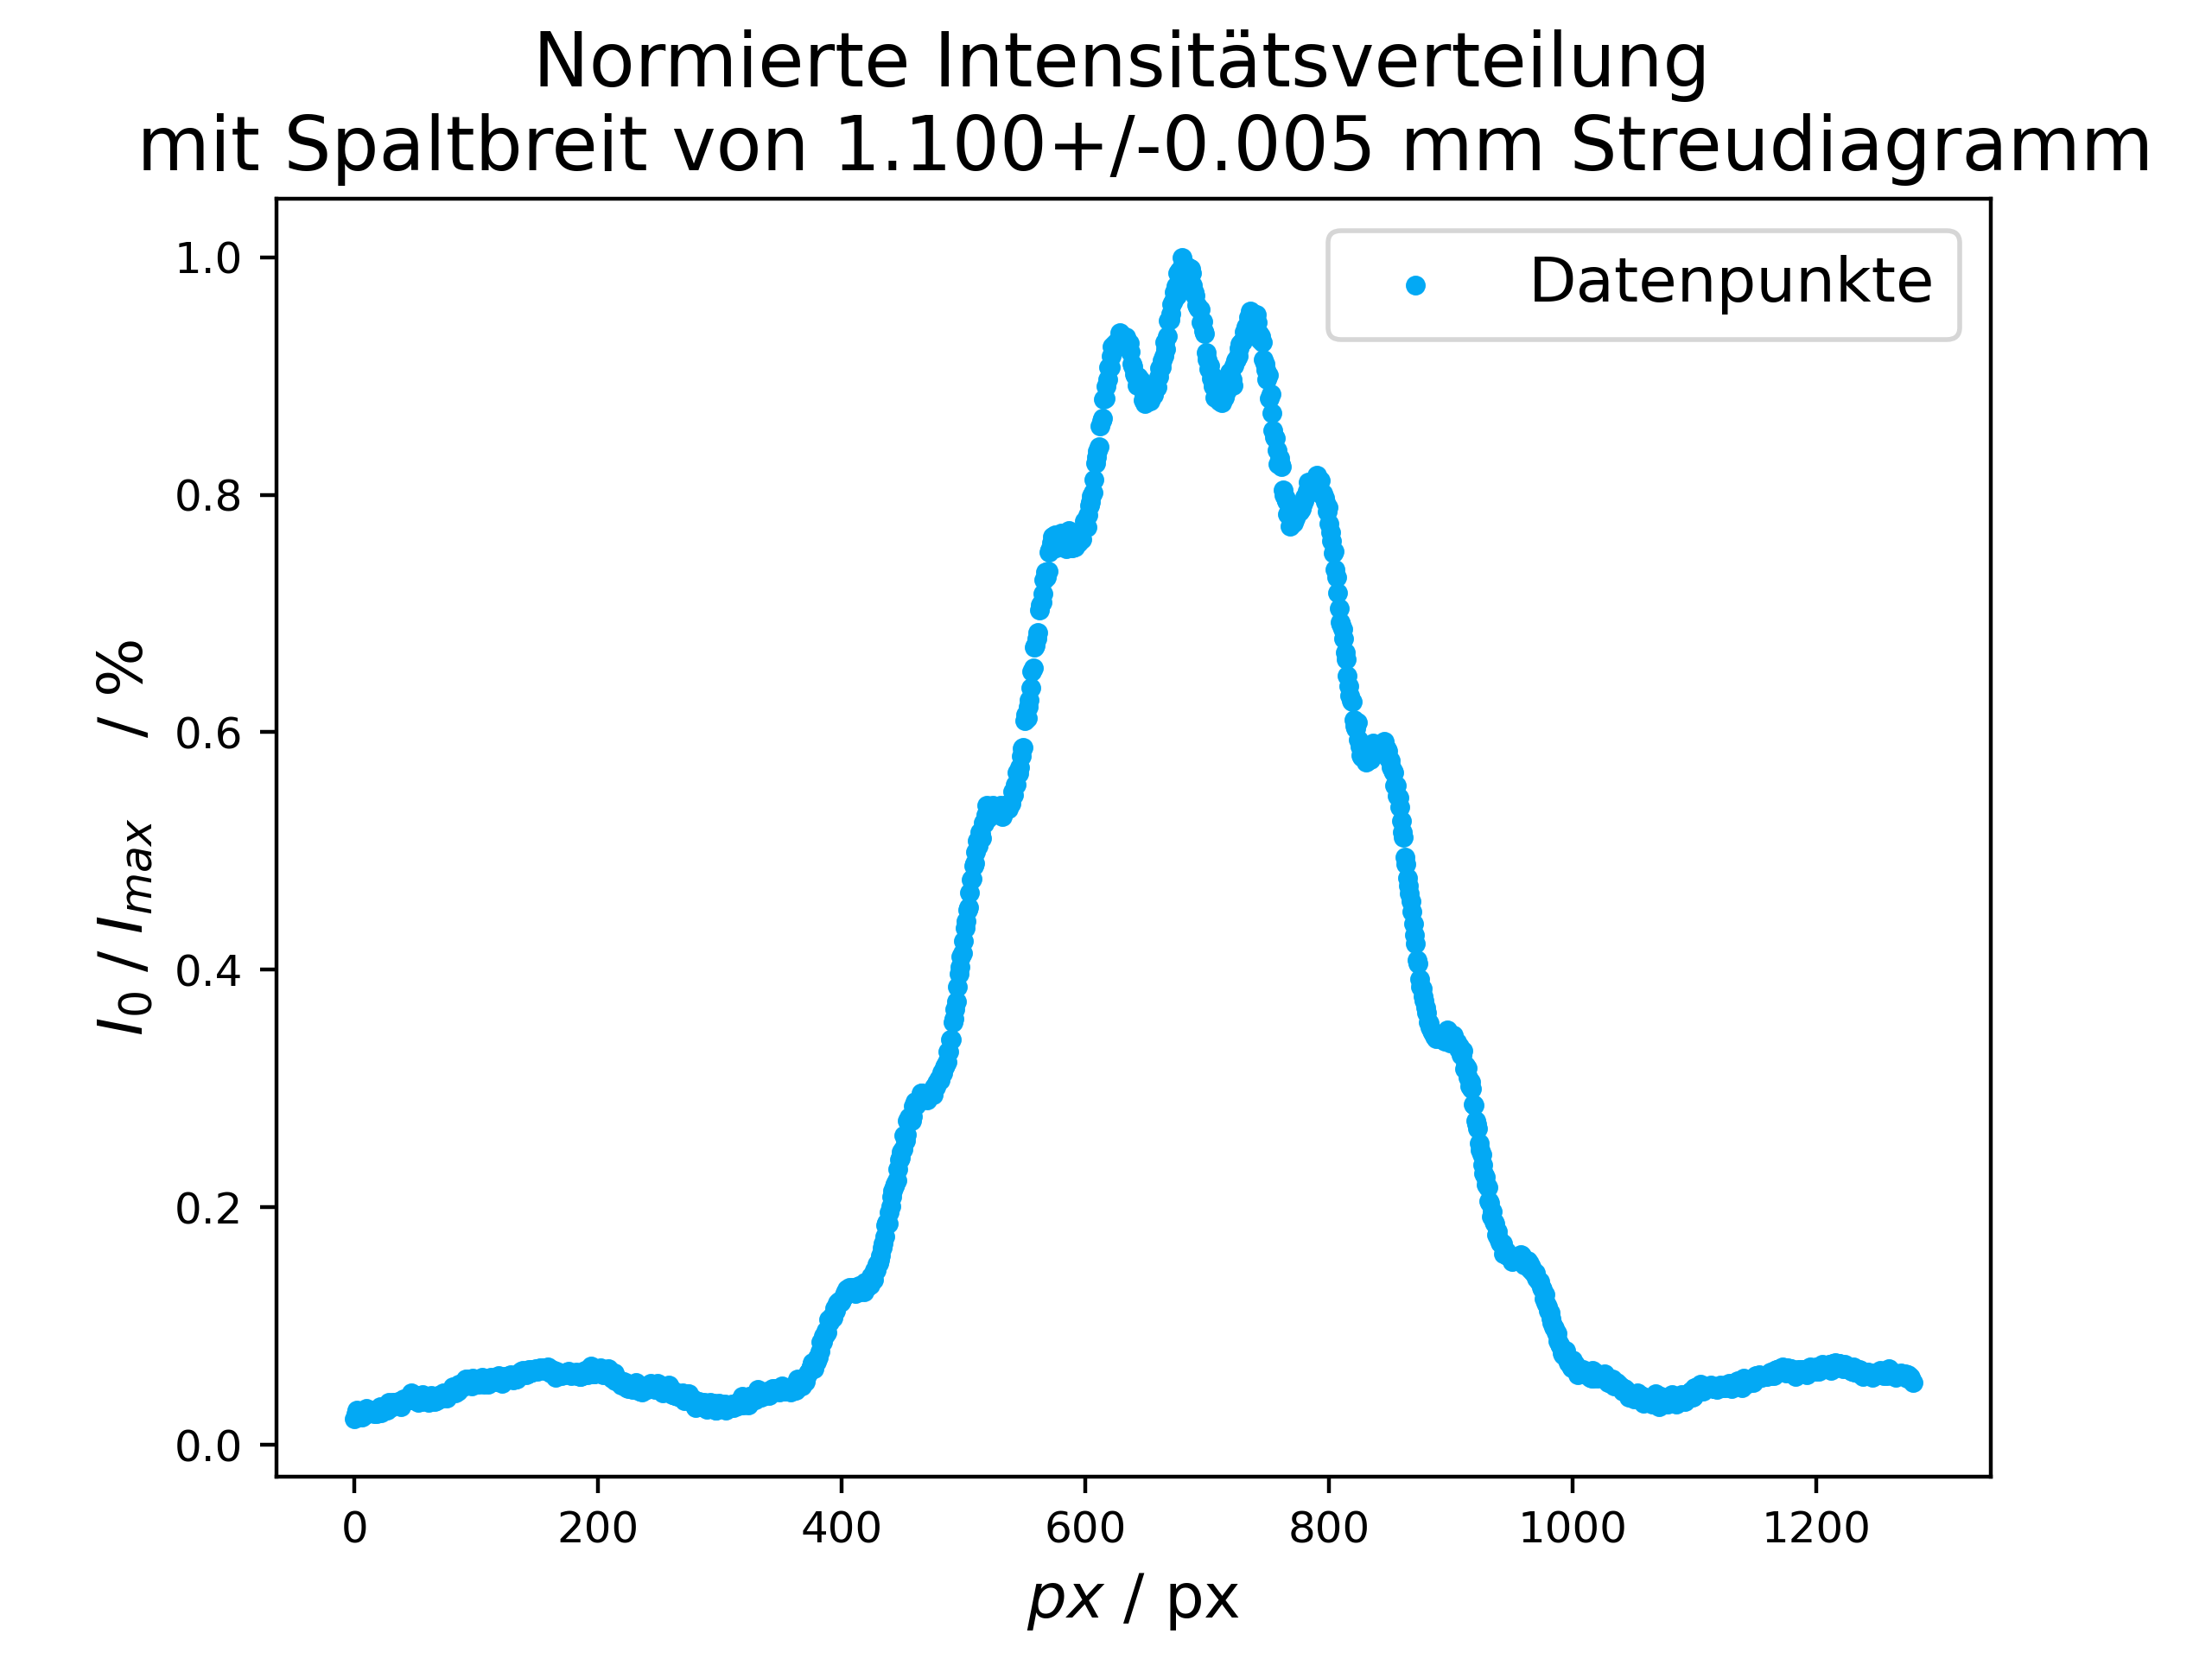
\includegraphics[width=\textwidth]{auswertung/0_89konstrast}
		\captionbelowof{figure}{geplotteter Grauwert \\ aufgetragen zu jeweiligen Pixelnummer \\ bei einer Spaltbreite von \SI{1.100(5)}{mm}}
	\end{minipage}
	\vspace{2mm}
	\begin{minipage}[t]{0.50\textwidth}
		\centering
		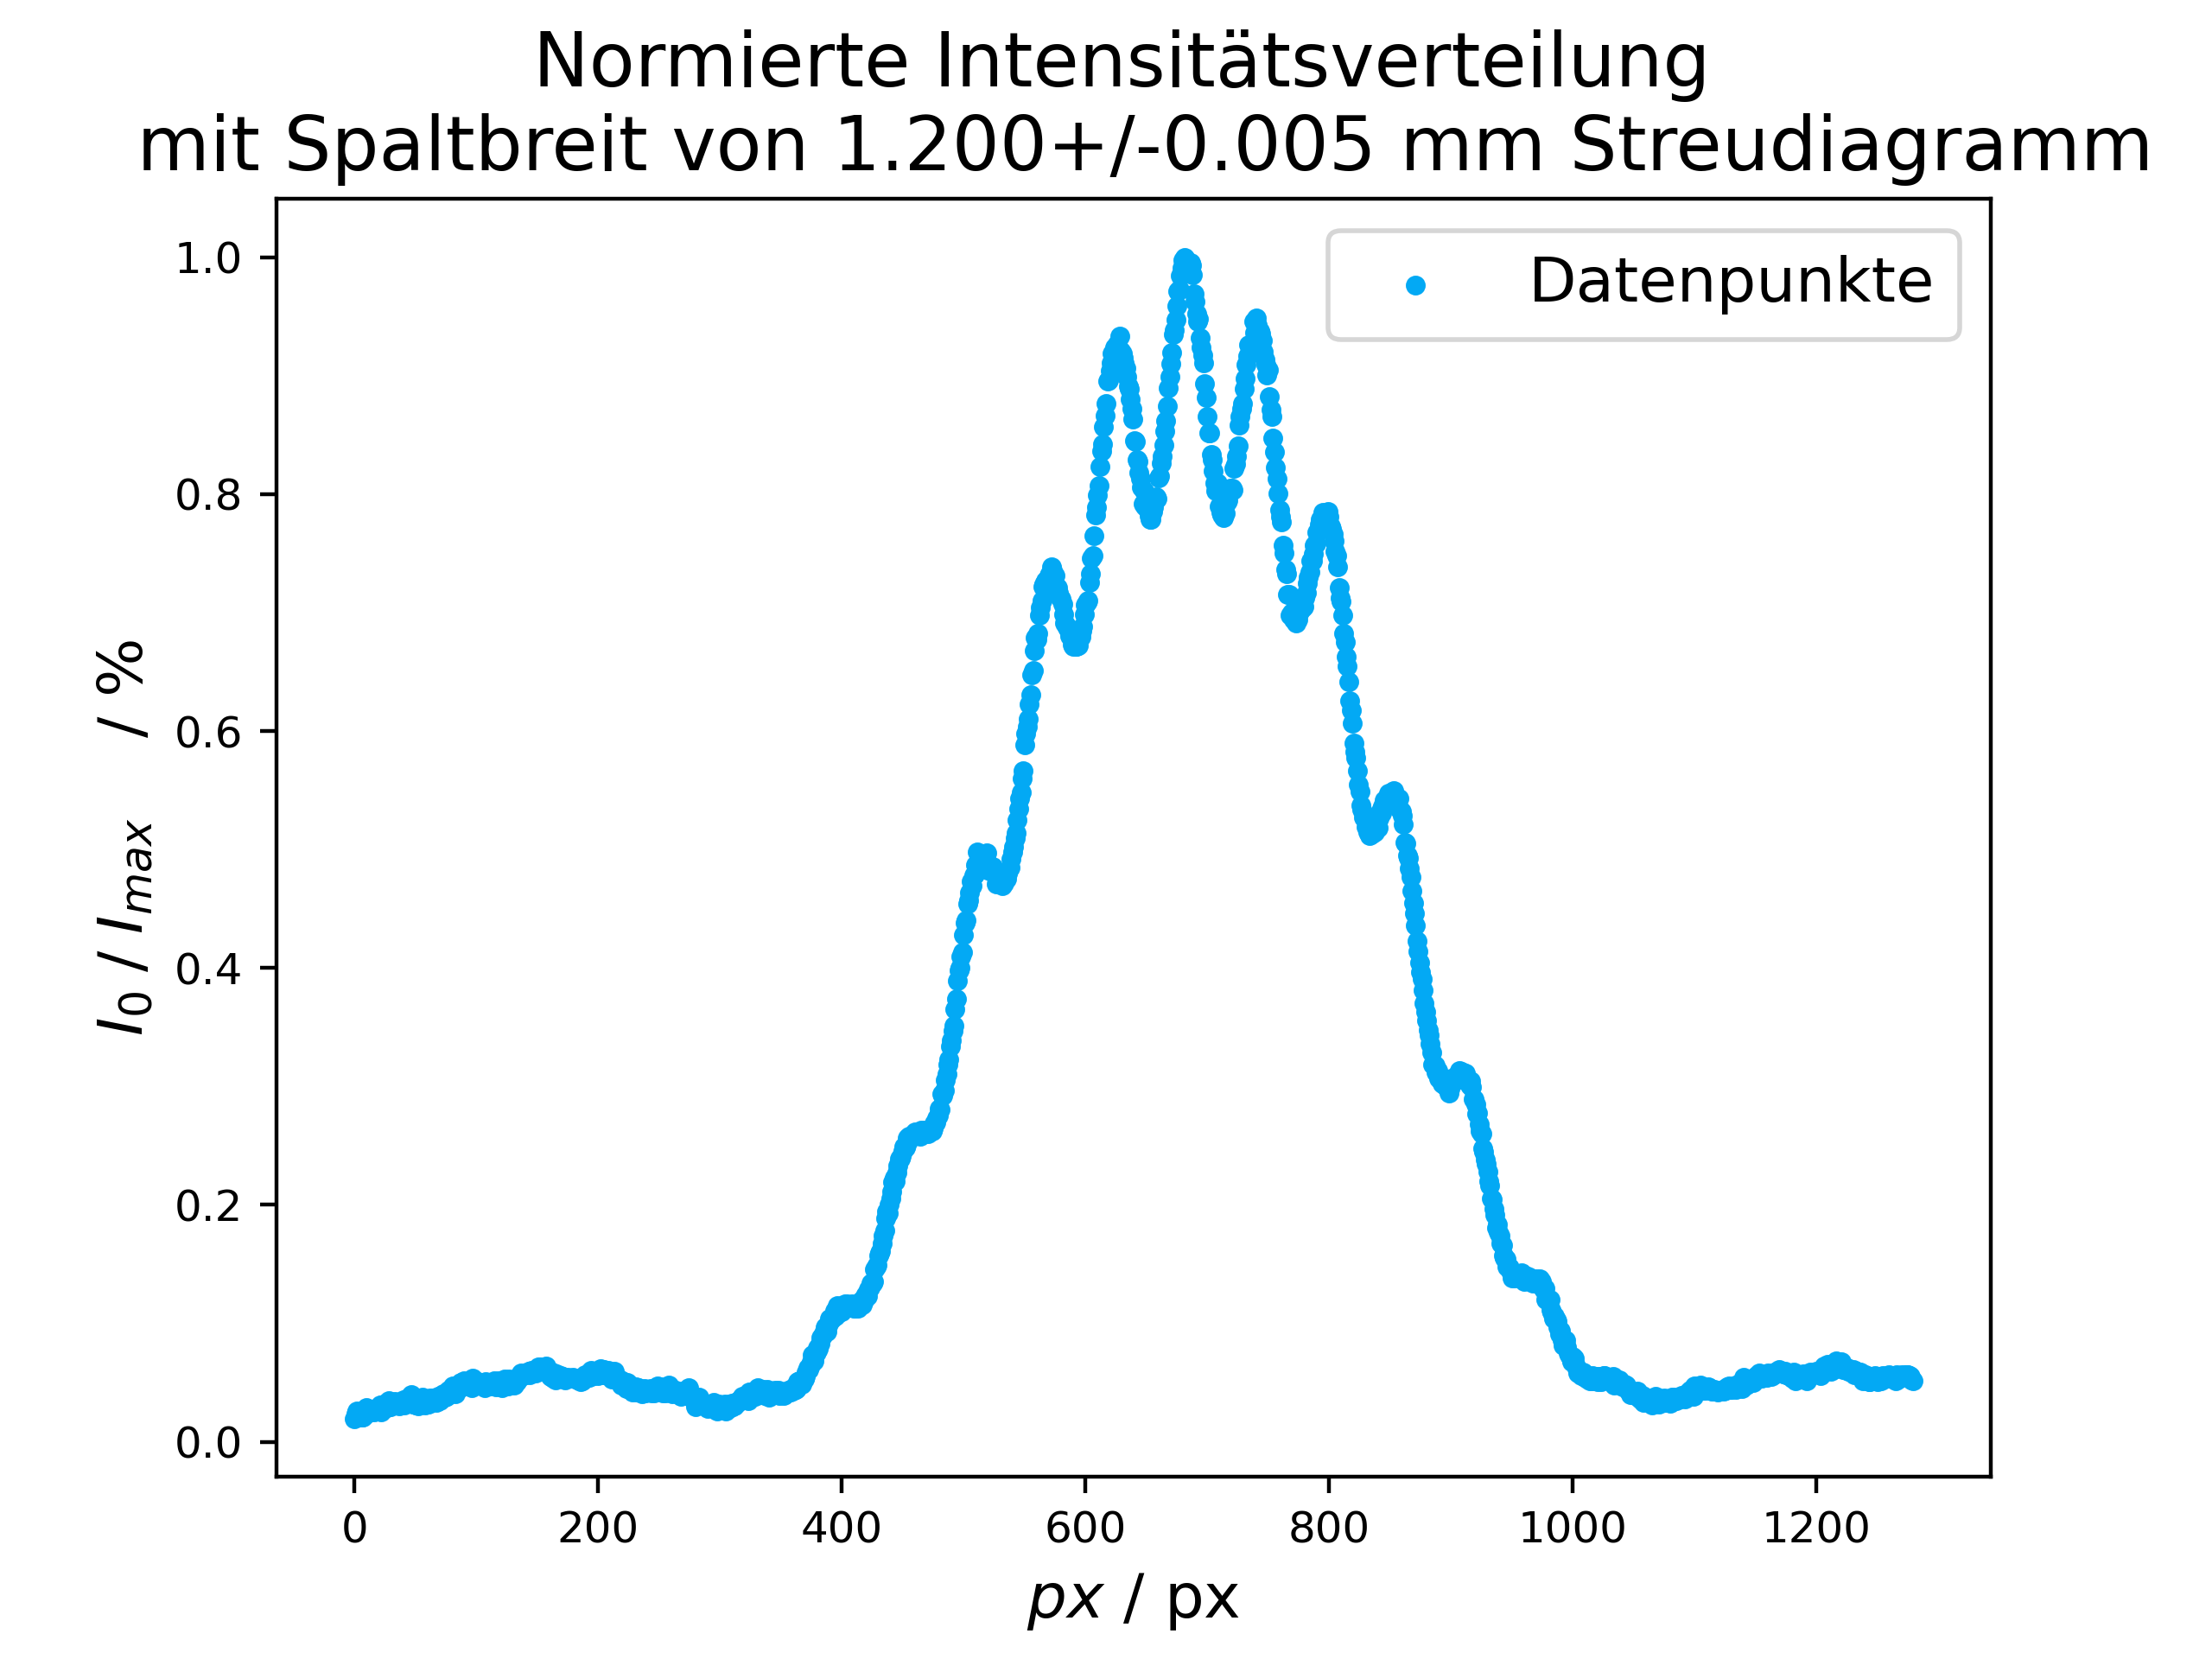
\includegraphics[width=\textwidth]{auswertung/0_99konstrast}
		\captionof{figure}{geplotteter Grauwert \\ aufgetragen zu jeweiligen Pixelnummer \\ bei einer Spaltbreite von \SI{1.200(5)}{mm}}
	\end{minipage}
	\vspace{1em}
\end{minipage}

\begin{minipage}{\textwidth}
	\begin{minipage}[t]{0.5\textwidth}
		\centering
		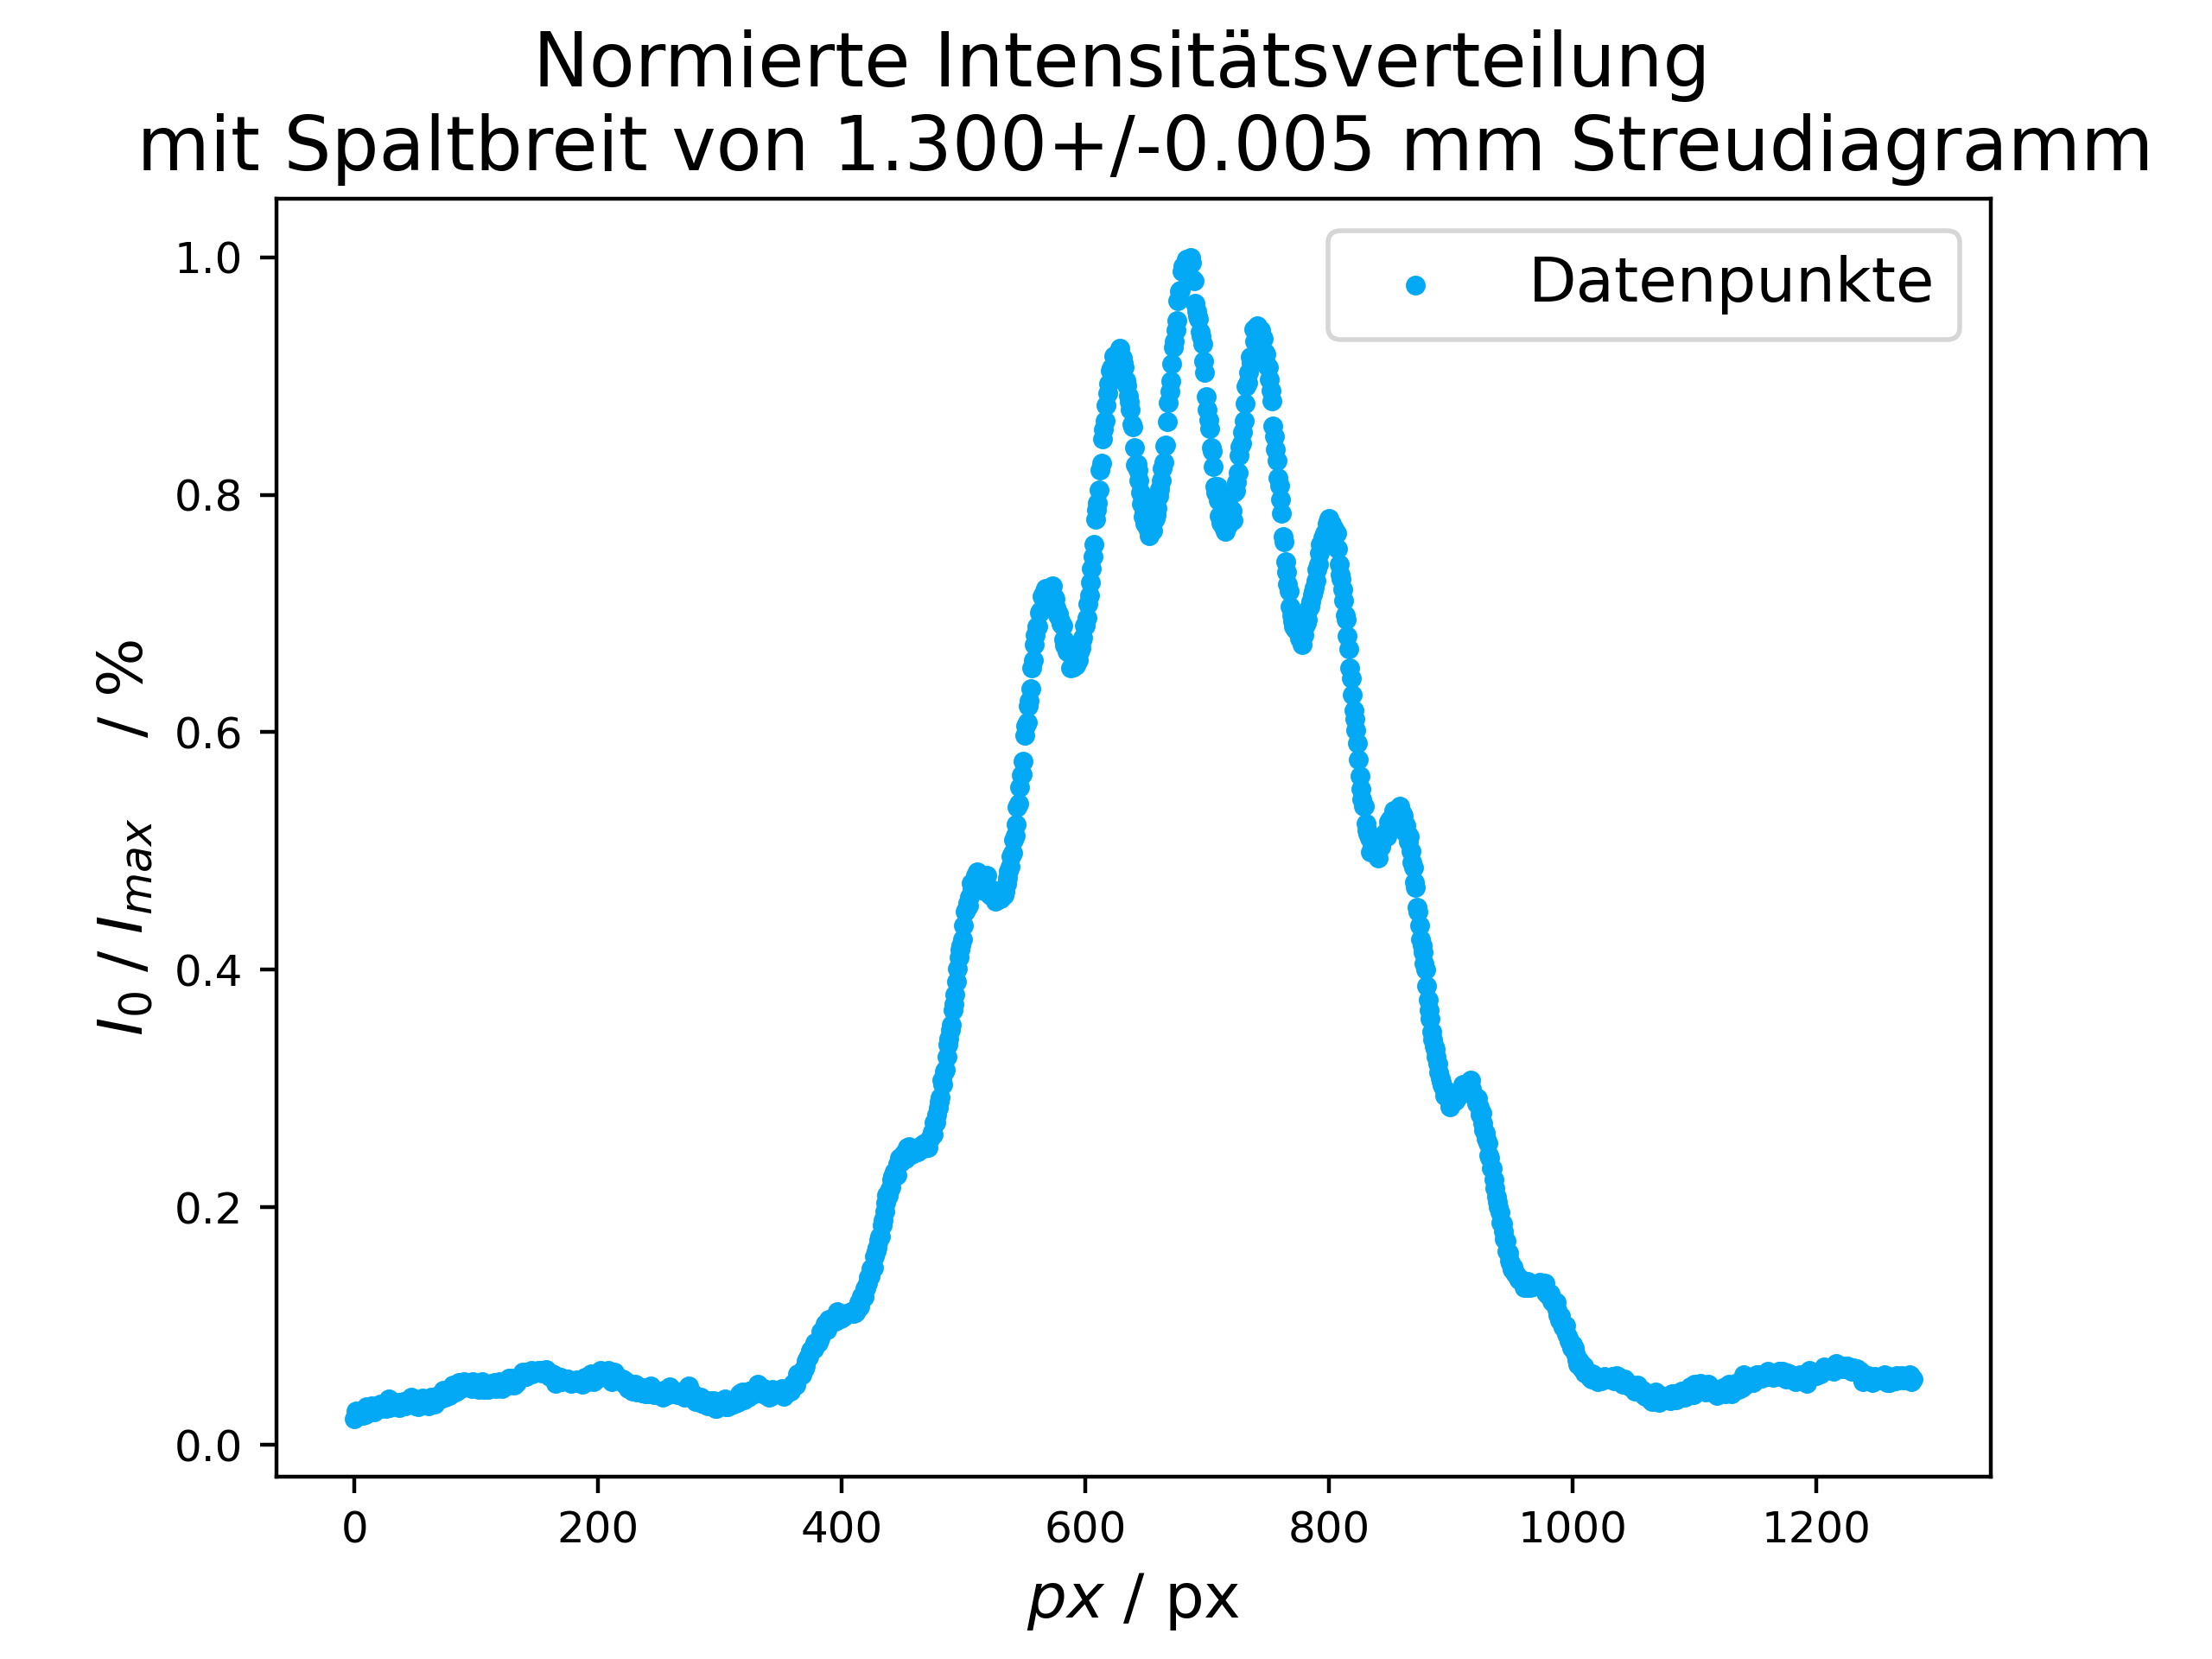
\includegraphics[width=\textwidth]{auswertung/1_09konstrast}
		\captionbelowof{figure}{geplotteter Grauwert \\ aufgetragen zu jeweiligen Pixelnummer \\ bei einer Spaltbreite von \SI{1.300(5)}{mm}}
	\end{minipage}
	\vspace{2mm}
	\begin{minipage}[t]{0.50\textwidth}
		\centering
		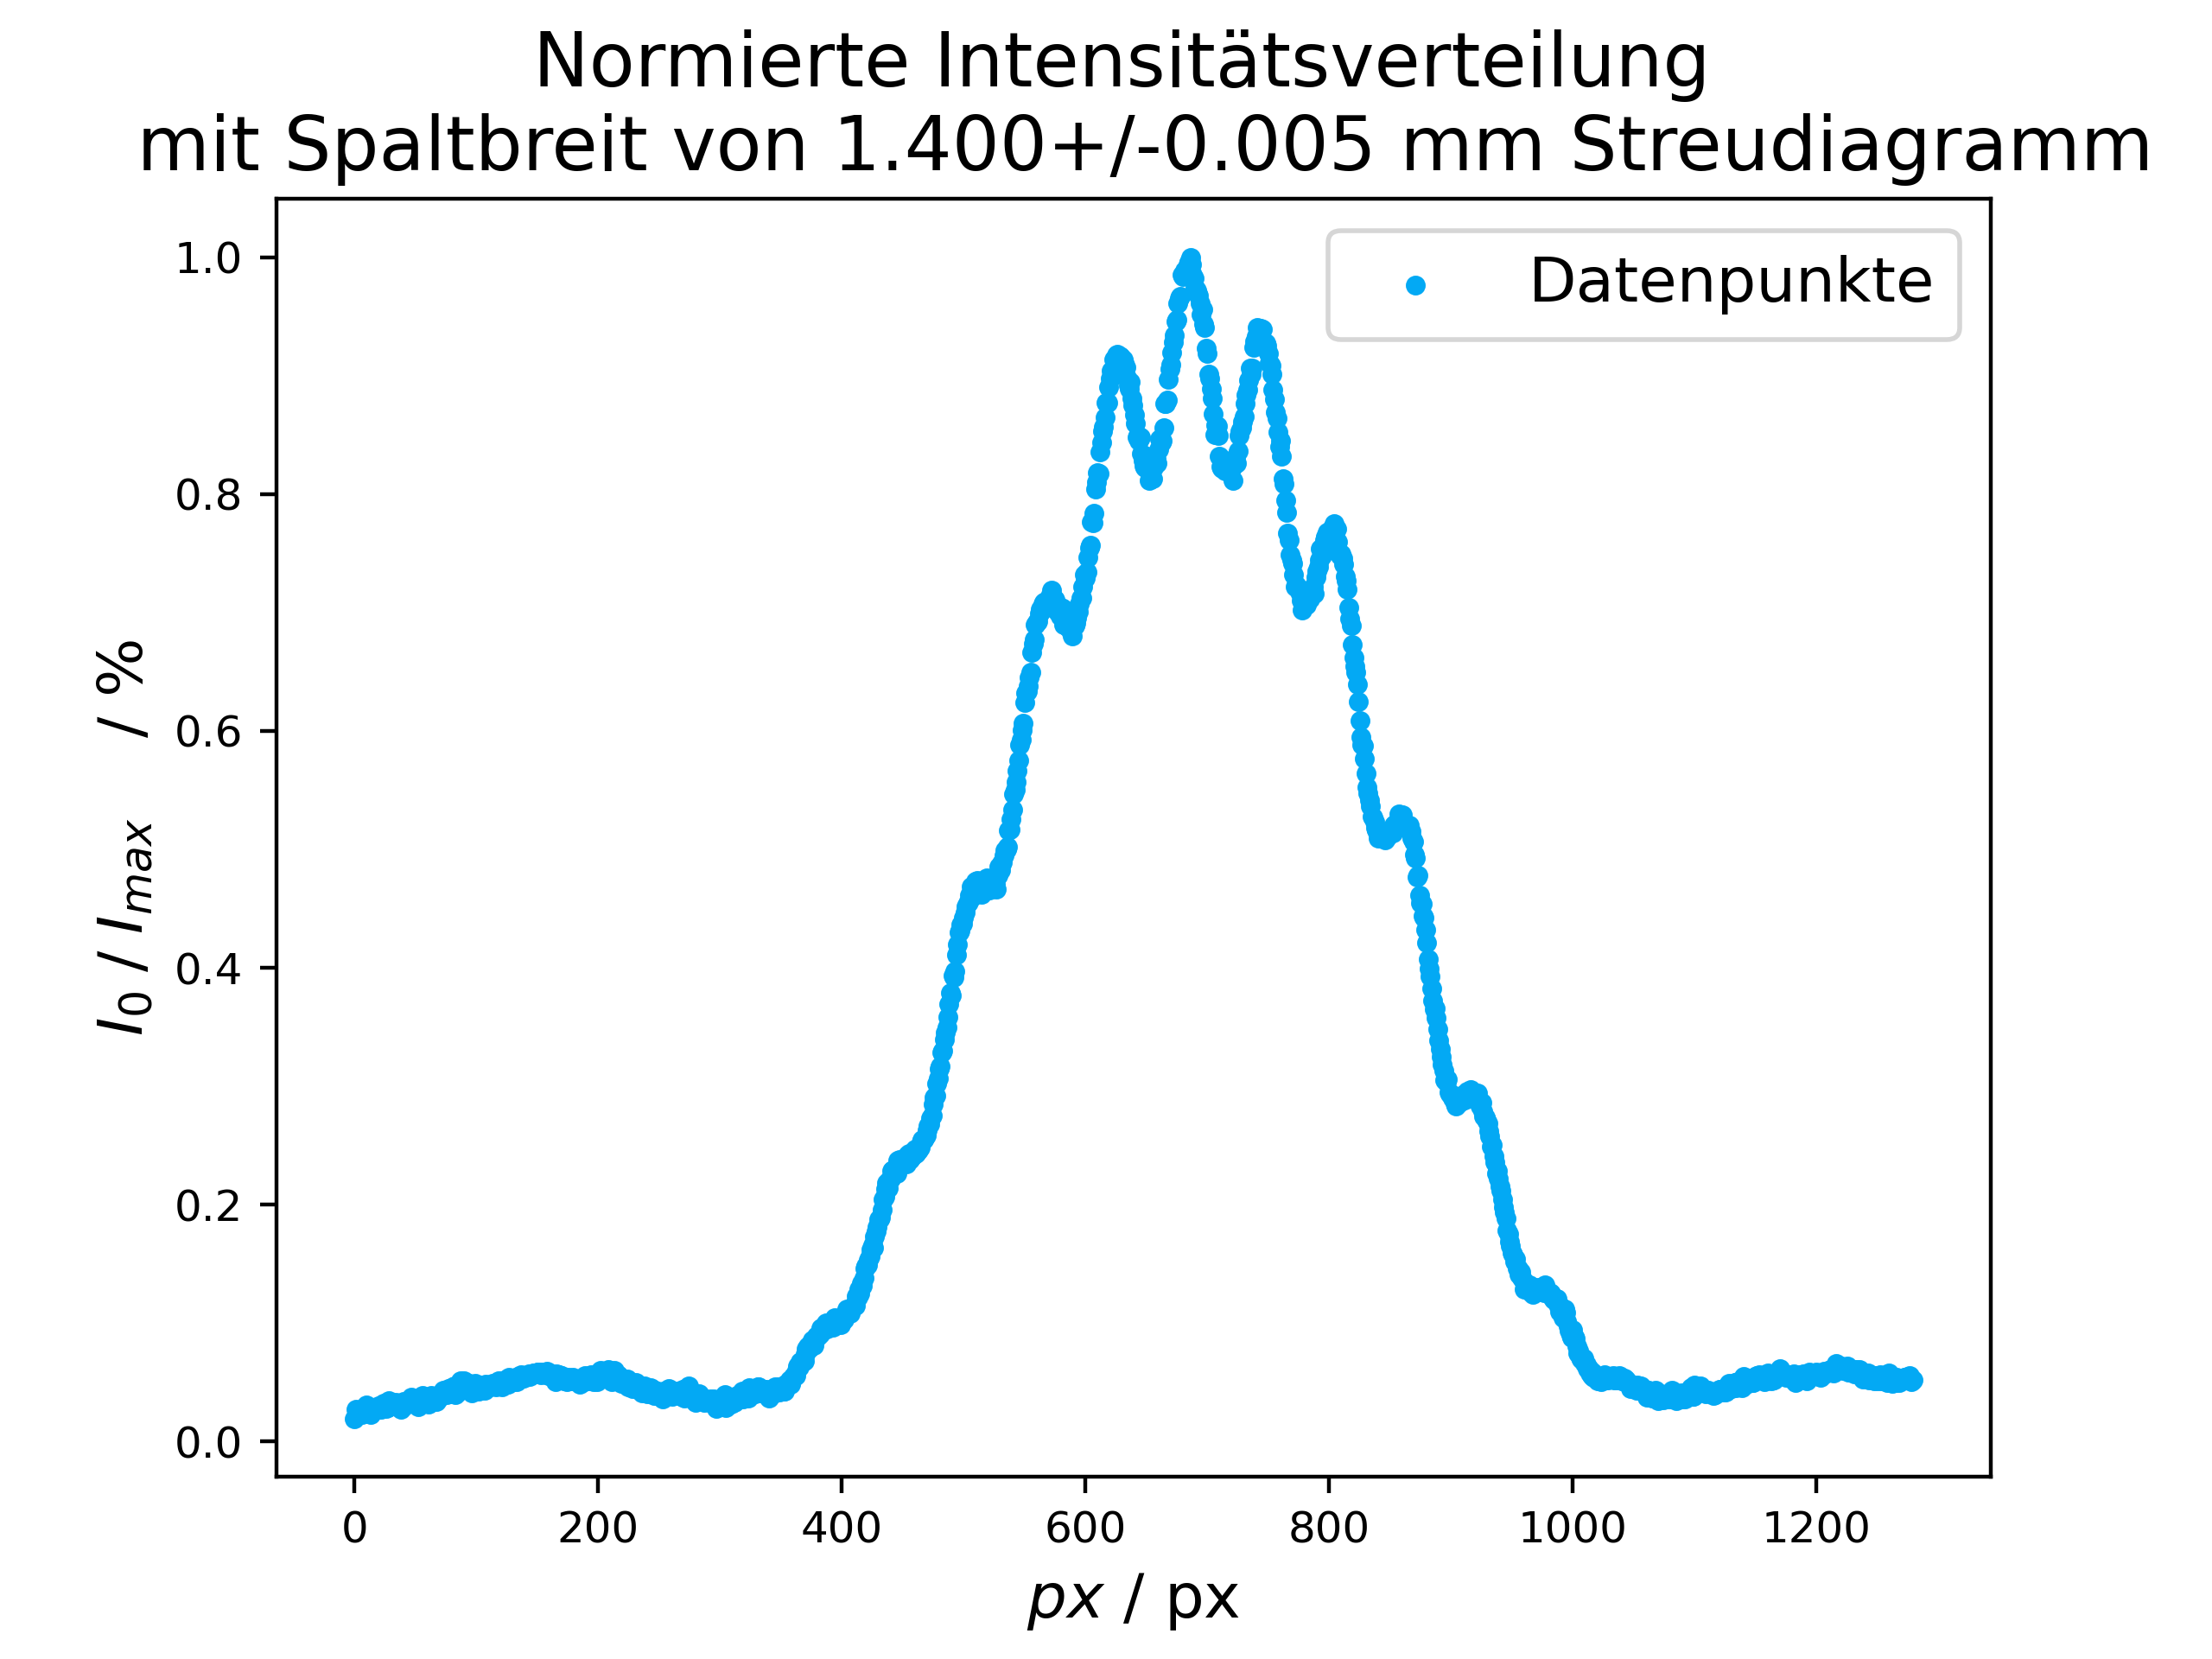
\includegraphics[width=\textwidth]{auswertung/1_19konstrast}
		\captionof{figure}{geplotteter Grauwert \\ aufgetragen zu jeweiligen Pixelnummer \\ bei einer Spaltbreite von \SI{1.400(5)}{mm}}
	\end{minipage}
	\vspace{1em}
\end{minipage}

\begin{minipage}{\textwidth}
	\begin{minipage}[t]{0.5\textwidth}
		\centering
		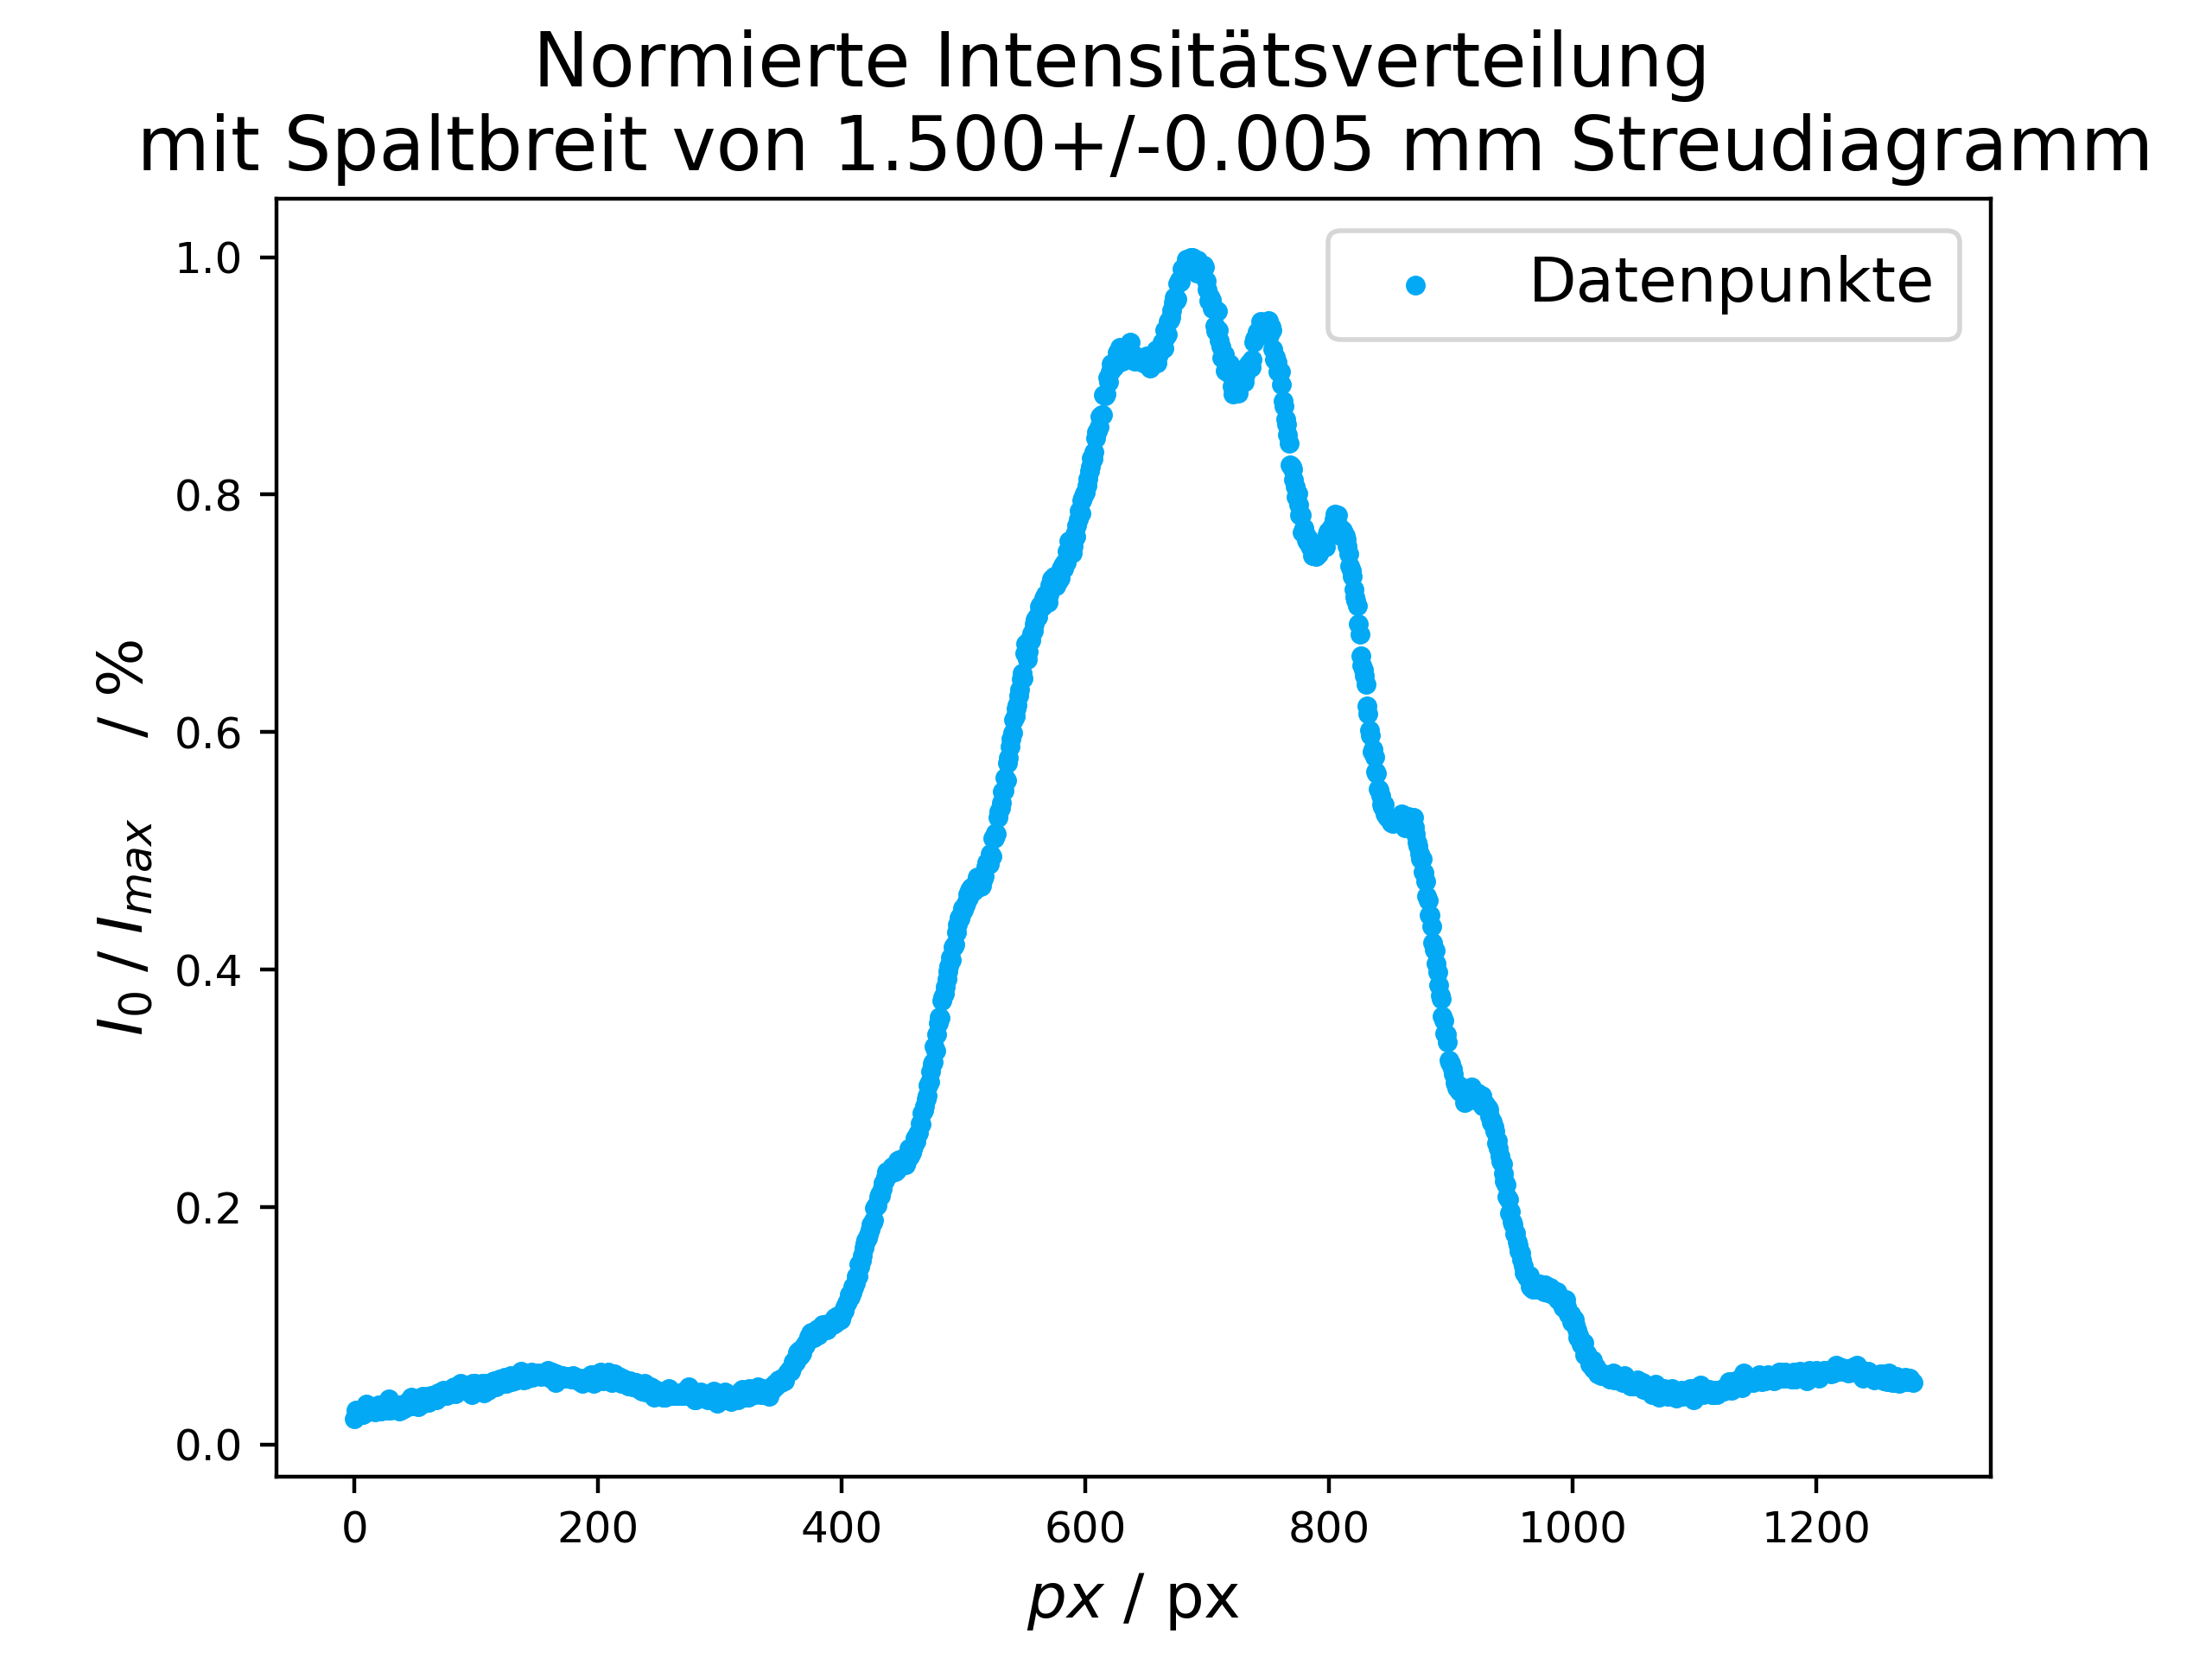
\includegraphics[width=\textwidth]{auswertung/1_29konstrast}
		\captionbelowof{figure}{geplotteter Grauwert \\ aufgetragen zu jeweiligen Pixelnummer \\ bei einer Spaltbreite von \SI{1.500(5)}{mm}}
	\end{minipage}
	\vspace{2mm}
	\begin{minipage}[t]{0.50\textwidth}
		\centering
		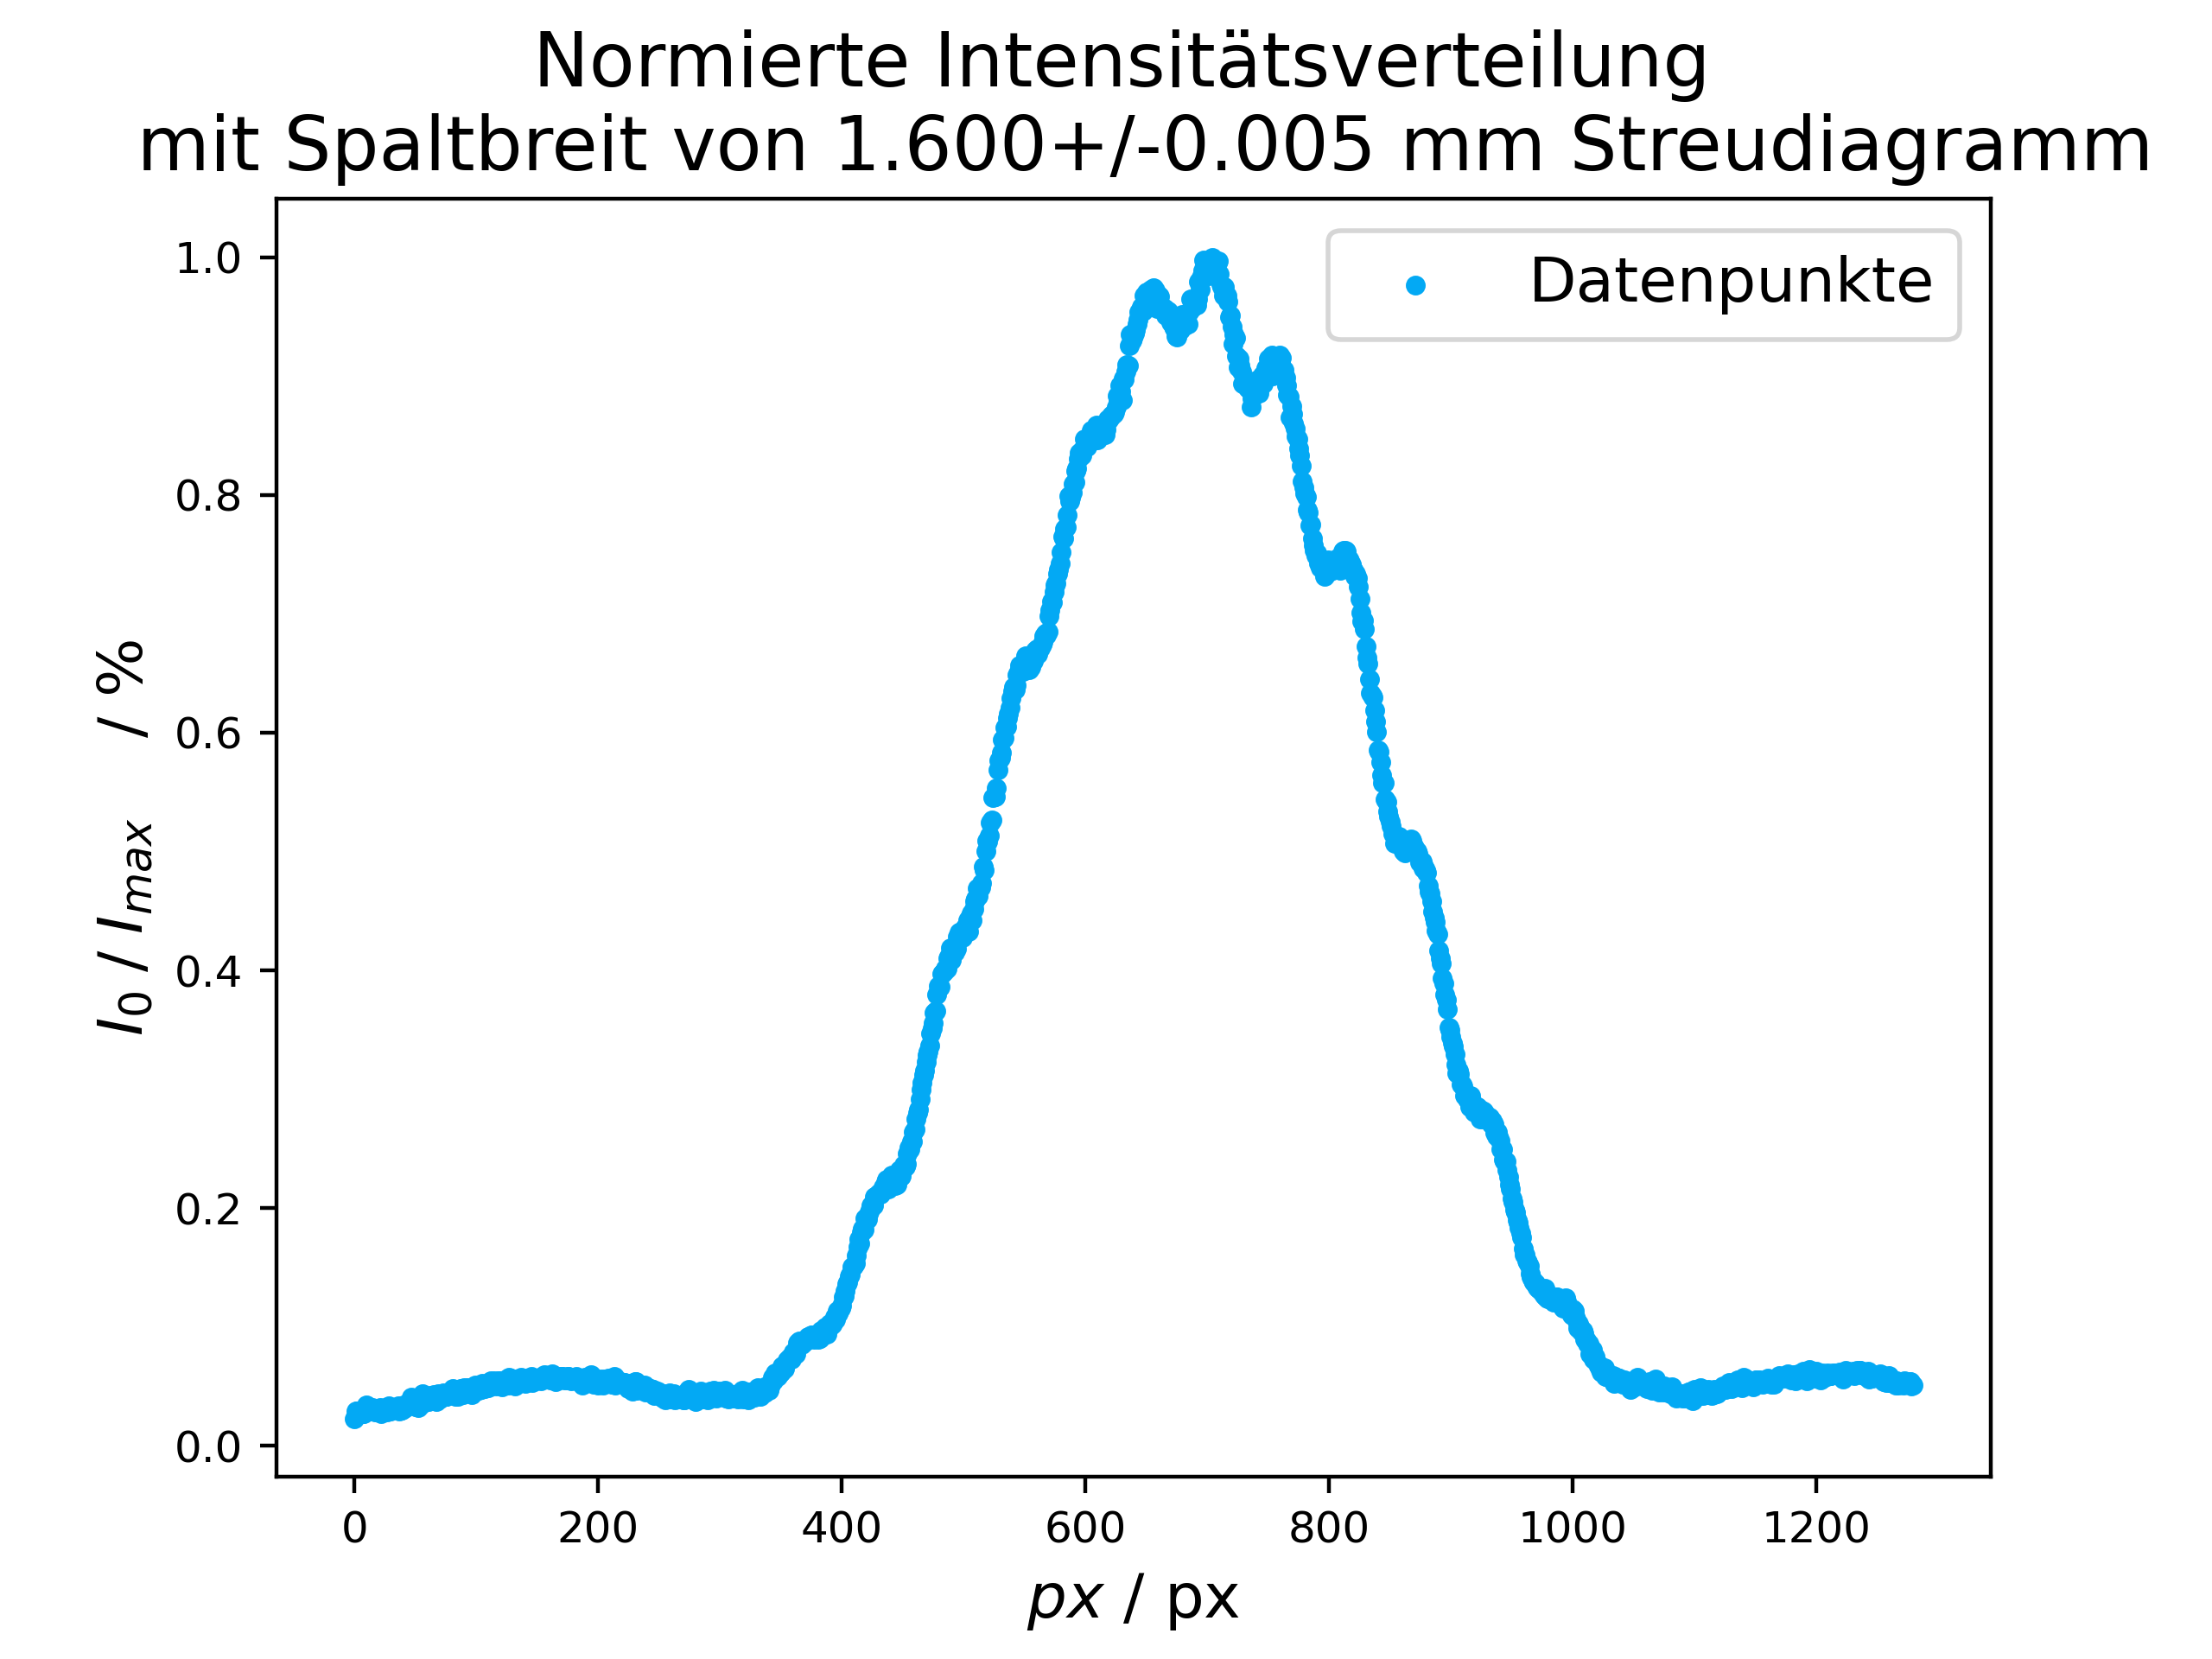
\includegraphics[width=\textwidth]{auswertung/1_39konstrast}
		\captionof{figure}{geplotteter Grauwert \\ aufgetragen zu jeweiligen Pixelnummer \\ bei einer Spaltbreite von \SI{1.600(5)}{mm}}
	\end{minipage}
	\vspace{1em}
\end{minipage}

\begin{center}
	\begin{minipage}[t]{0.5\textwidth}
		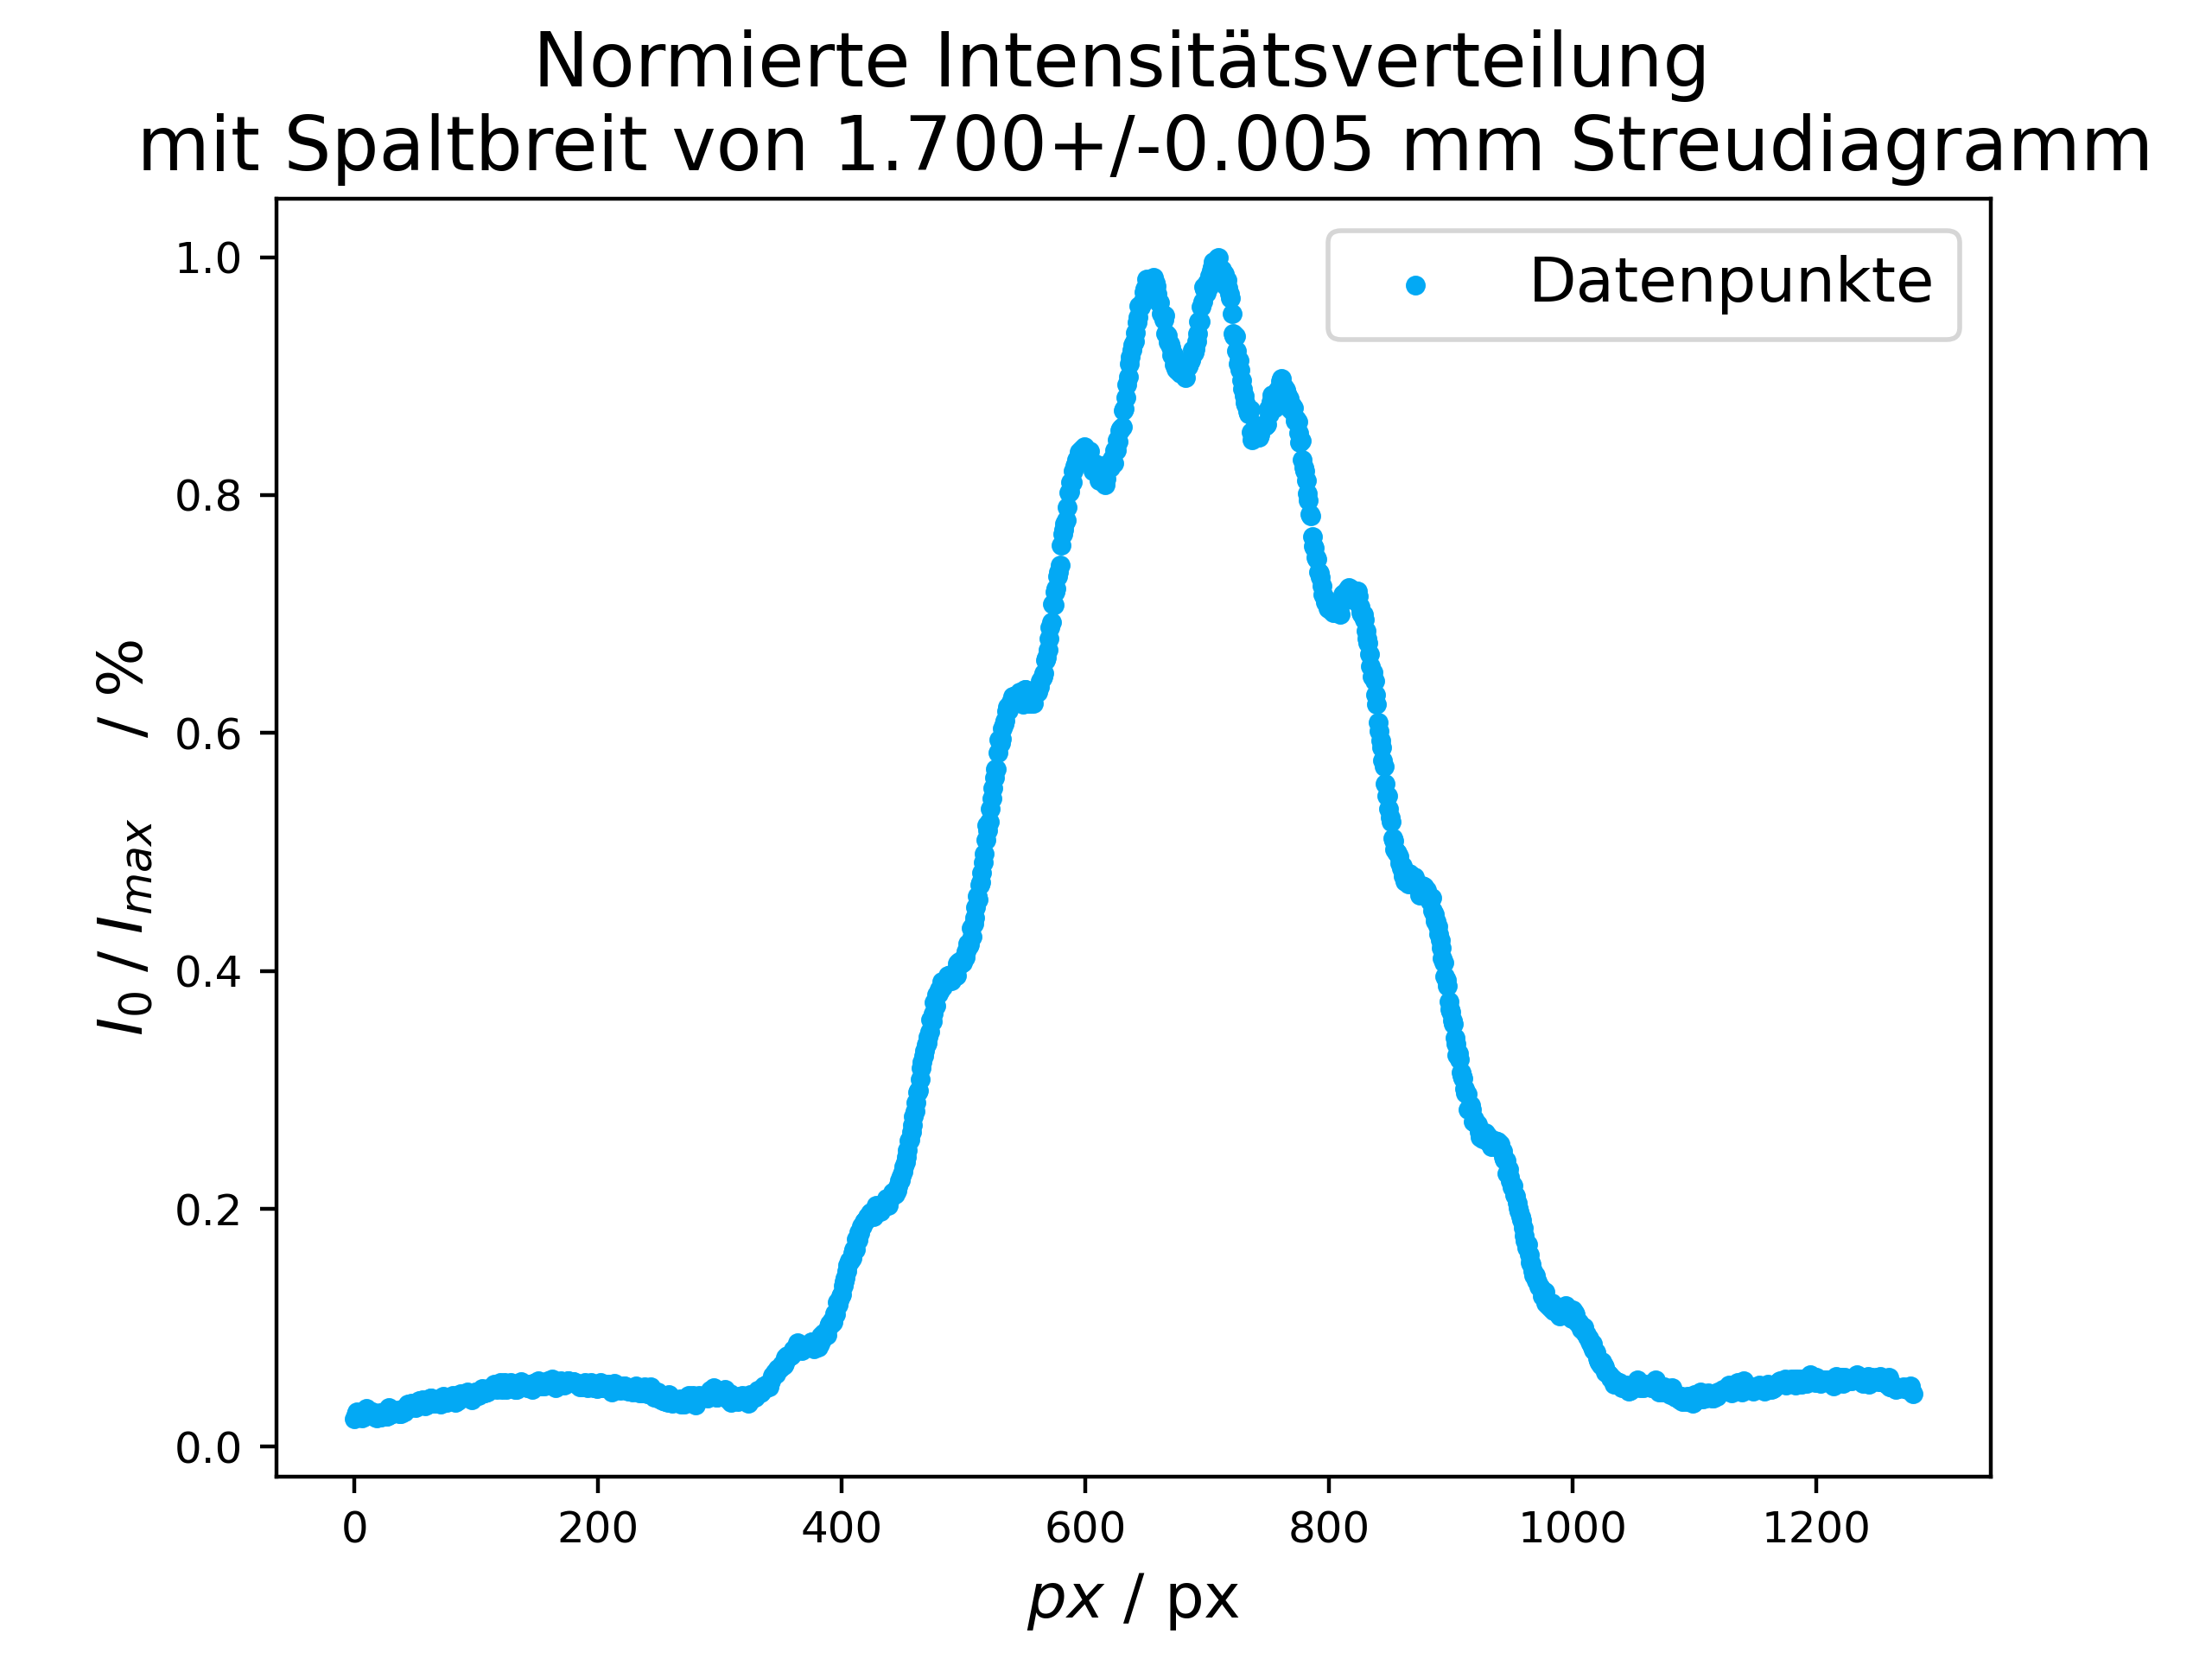
\includegraphics[width=\textwidth]{auswertung/1_49konstrast}
		\captionof{figure}{geplotteter Grauwert \\ aufgetragen zu jeweiligen Pixelnummer \\ bei einer Spaltbreite von \SI{1.700(5)}{mm}}
	\end{minipage}
\end{center}


\newpage



\subsection{Einfluss der spektralen Breite einer Lichtquelle auf das Interferenzmuster eines Doppelspalts}

Für Versuch 2 werden die verschiedenen Filter des Filterrads F in den Strahlengang gedreht. Diese sind in folgender \autoref{fig:filter} sichtbar.

\begin{center}
	\begin{minipage}[t]{0.7\textwidth}
		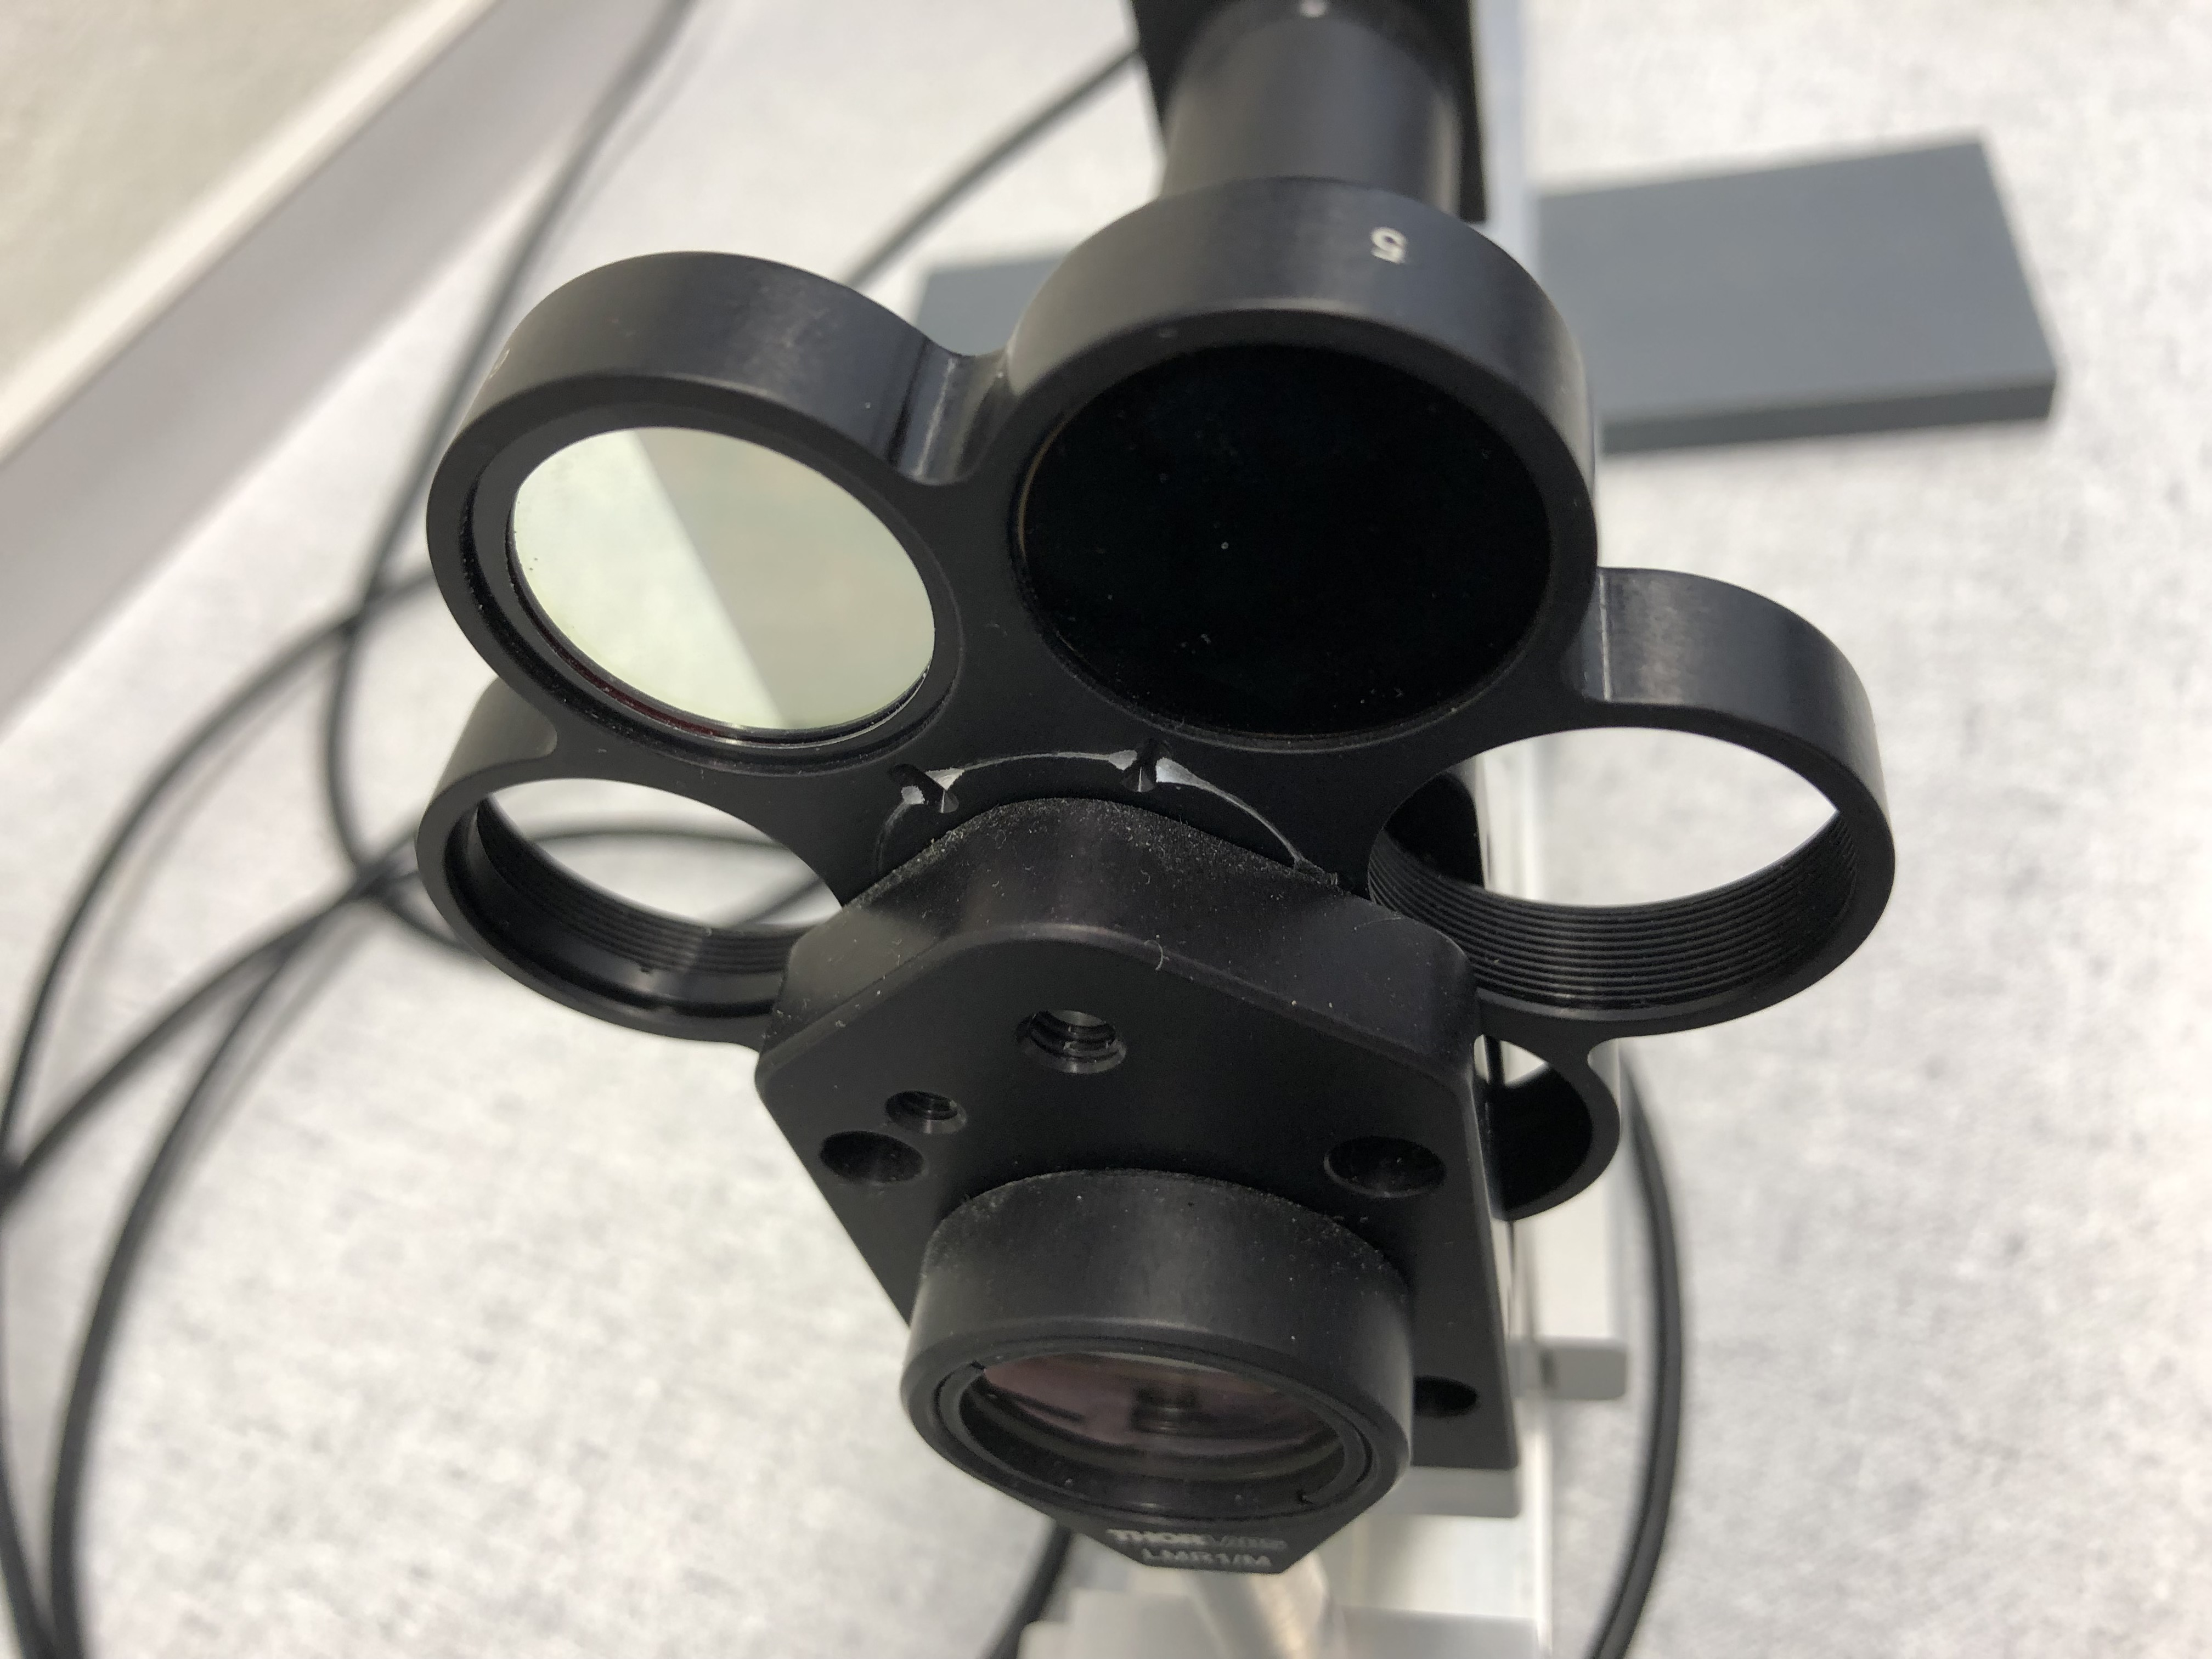
\includegraphics[width=\textwidth]{filter}
		\captionof{figure}{verschiedene Filter an Filterrad}
		\label{fig:filter}
	\end{minipage}
\end{center}

\noindent Der dunkle Filter, bei dem in der \autoref{fig:filter} die 5 sichtbar ist, ist
ein Langpassfilter, der ab einer Wellenlänge von ca. \SI{710}{nm} aktiv wird.
Der Filter links daneben ist der Bandpassfilter von \SI{633}{nm}. Die anderen 4
Positionen im Filterrad sind leer.

\noindent Die genaue Transmission der Filter ist in folgender \autoref{fig:transmission} veranschaulicht.

\begin{center}
	\begin{minipage}[t]{0.5\textwidth}
		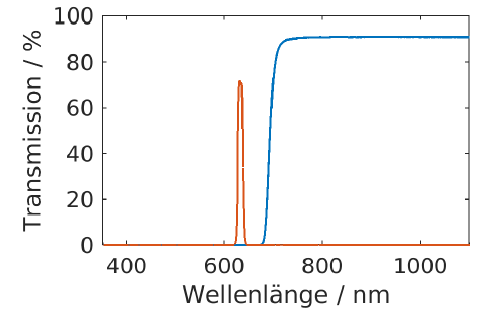
\includegraphics[width=\textwidth]{transmission}
		\captionof{figure}{Abbildung der Transmissionen der Filter \\ Orange
			beschreibt dabei den Bandpassfilter, während die blaue Kurve den
			Langpassfilter beschreibt \cite{vorlageinterfero}}
		\label{fig:transmission}
	\end{minipage}
\end{center}

\noindent Nun werden wieder, wie bereits unter Versuch 1 beschrieben die Interferenzmuster mit den unterschiedlichen Filtern mithilfe der  Computersoftware ``IC Capture`` aufgenommen, was in folgenden 3 Abbildungen sichtbar ist. der Abstand des Doppelspalts war wieder, wie zuvor, \SI{0.430(5)}{mm}, während für die Spaltbreite ein Abstand von \SI{0.200(5)}{mm}, mit Berücksichtigung der Offsets, gewählt wurde. Es wurde wieder ein Bild des gesamten Bildschirms abgebildet, um die Werte die beispielsweise für die ``Exposure`` angegeben wurden, festzuhalten.

\begin{center}
	\begin{minipage}[t]{\textwidth}
		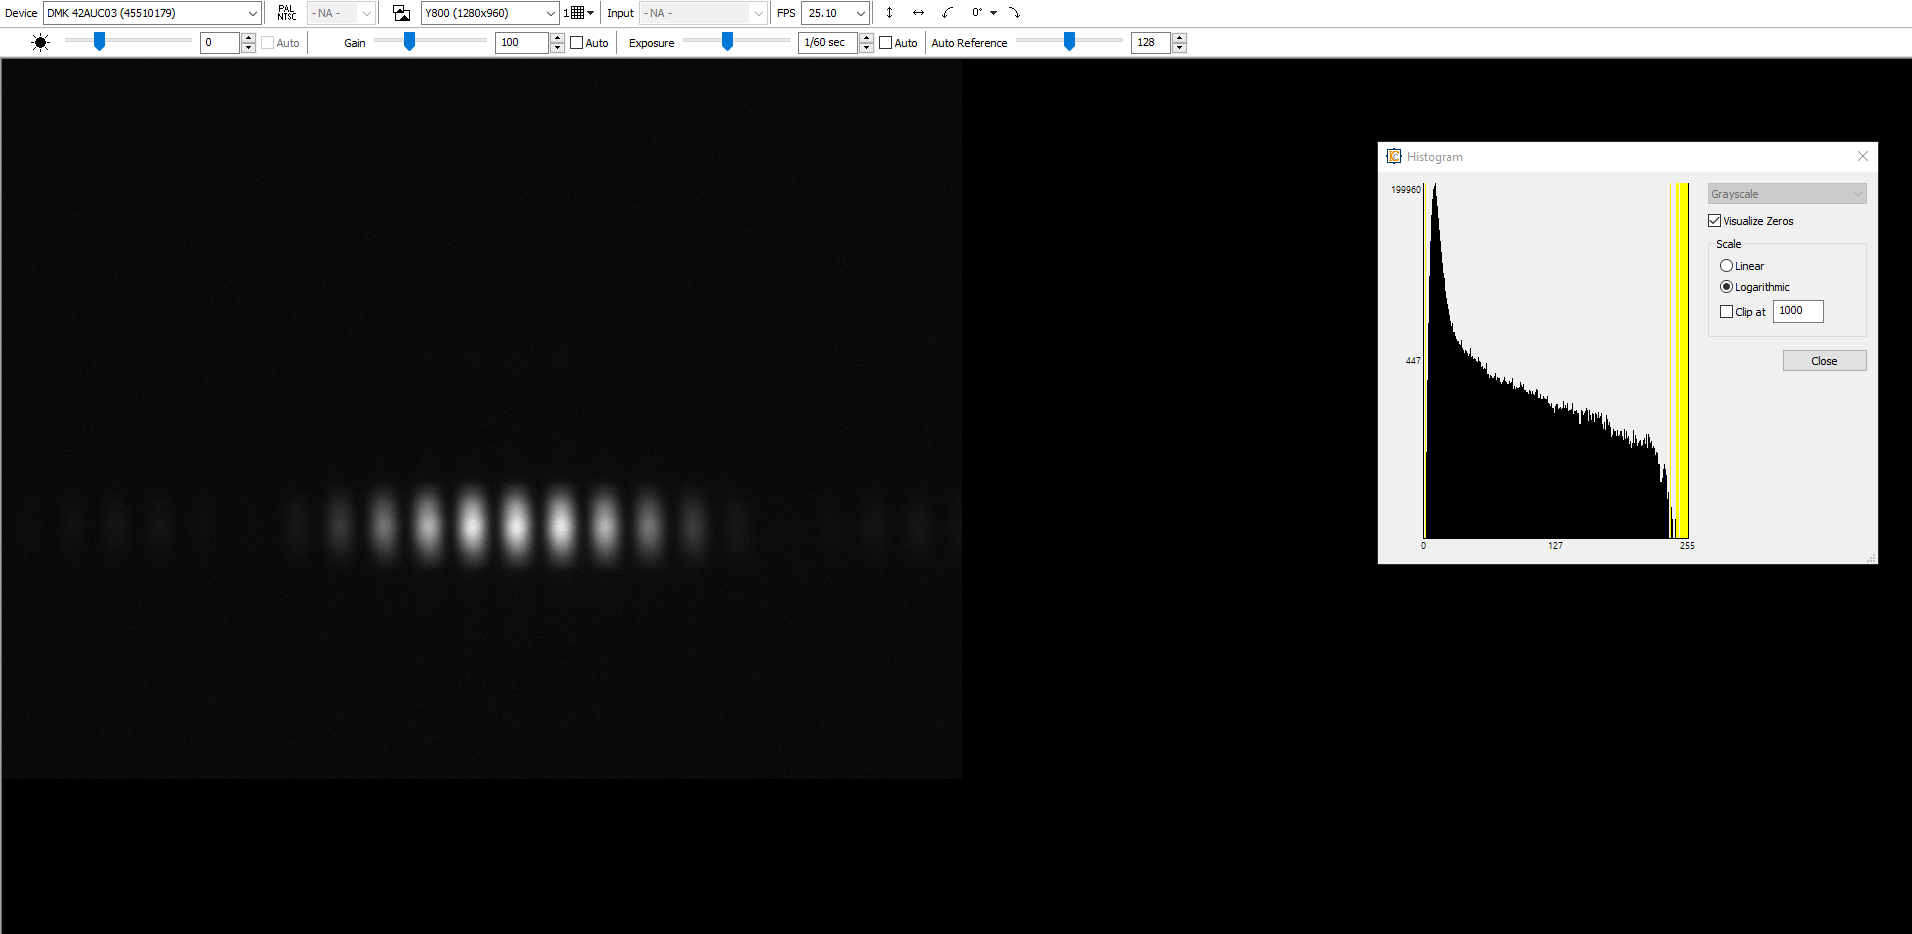
\includegraphics[width=\textwidth]{Interfero/Versuch2/bandpassfilter}
		\captionof{figure}{Interferenzmuster bei einer Spaltbreite von
			\SI{0.200(5)}{mm} unter Verwendung des Bandpassfilters und einem
			Doppelspalt mit \SI{0.430(5)}{mm}}
		\label{fig:bandpassfilter}
	\end{minipage}
\end{center}

\begin{center}
	\begin{minipage}[t]{\textwidth}
		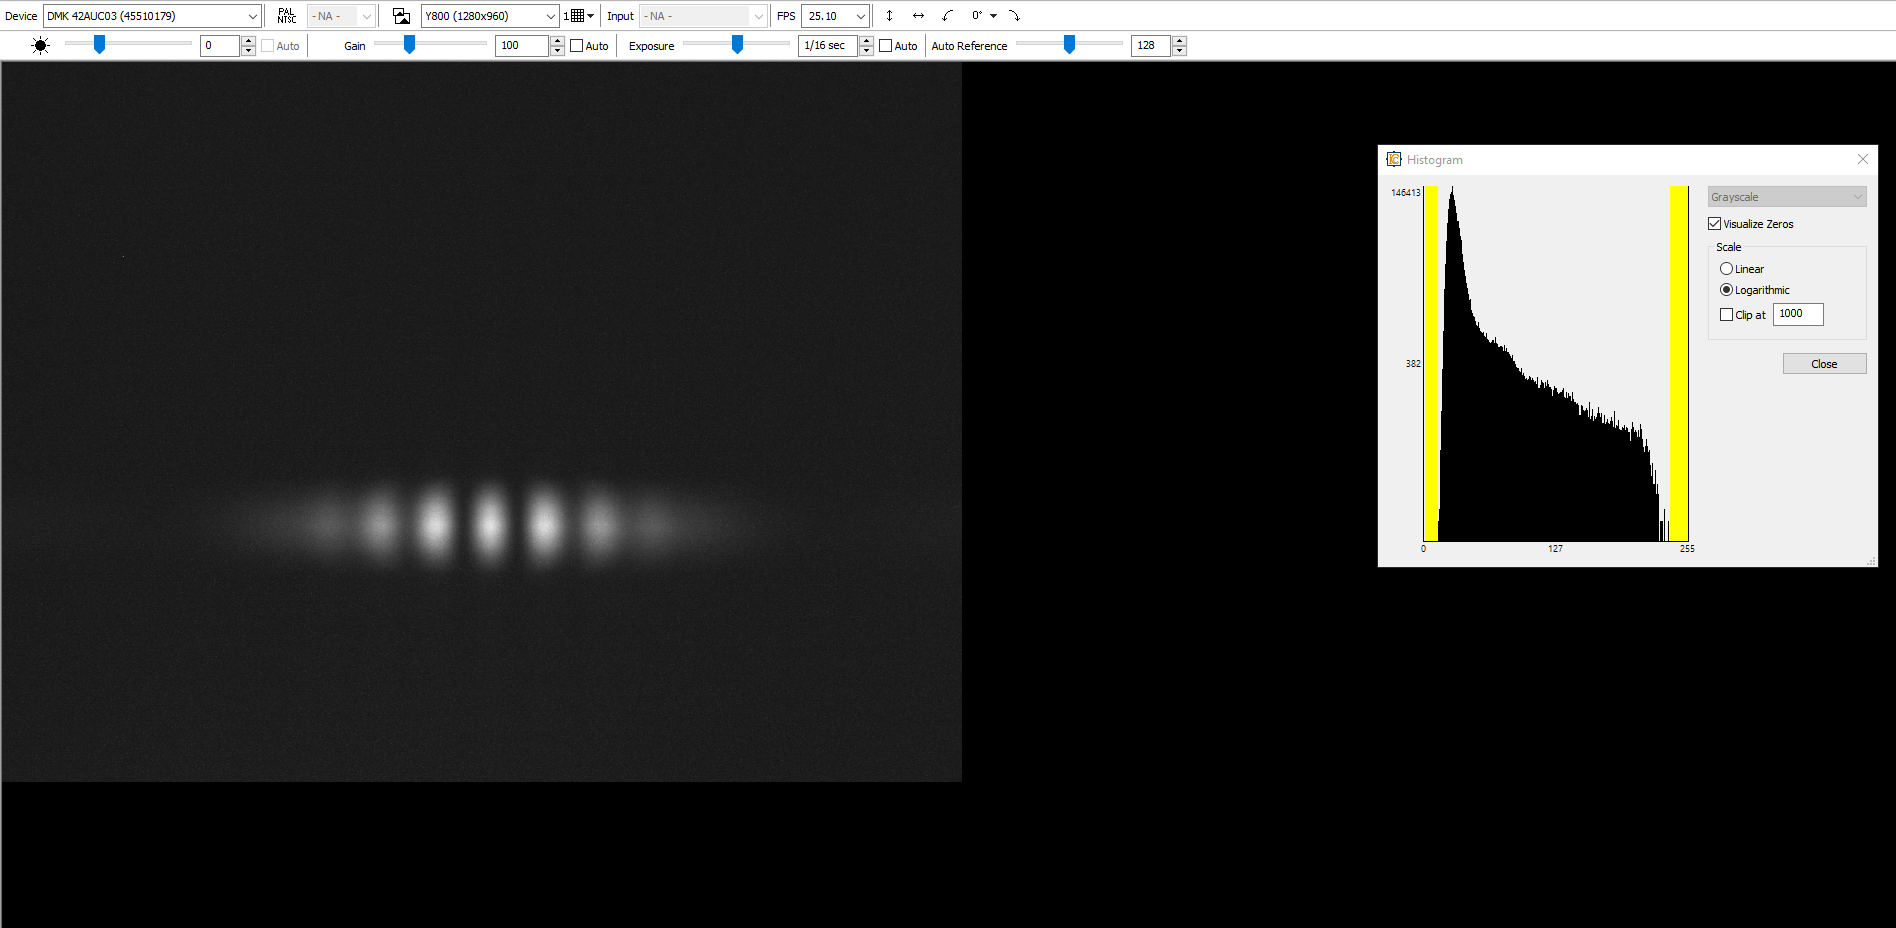
\includegraphics[width=\textwidth]{Interfero/Versuch2/langpassfilter}
		\captionof{figure}{Interferenzmuster bei einer Spaltbreite von
			\SI{0.200(5)}{mm} unter Verwendung des Langpassfilters und einem
			Doppelspalt mit \SI{0.430(5)}{mm}}
		\label{fig:langpassfilter}
	\end{minipage}
\end{center}

\begin{center}
	\begin{minipage}[t]{\textwidth}
		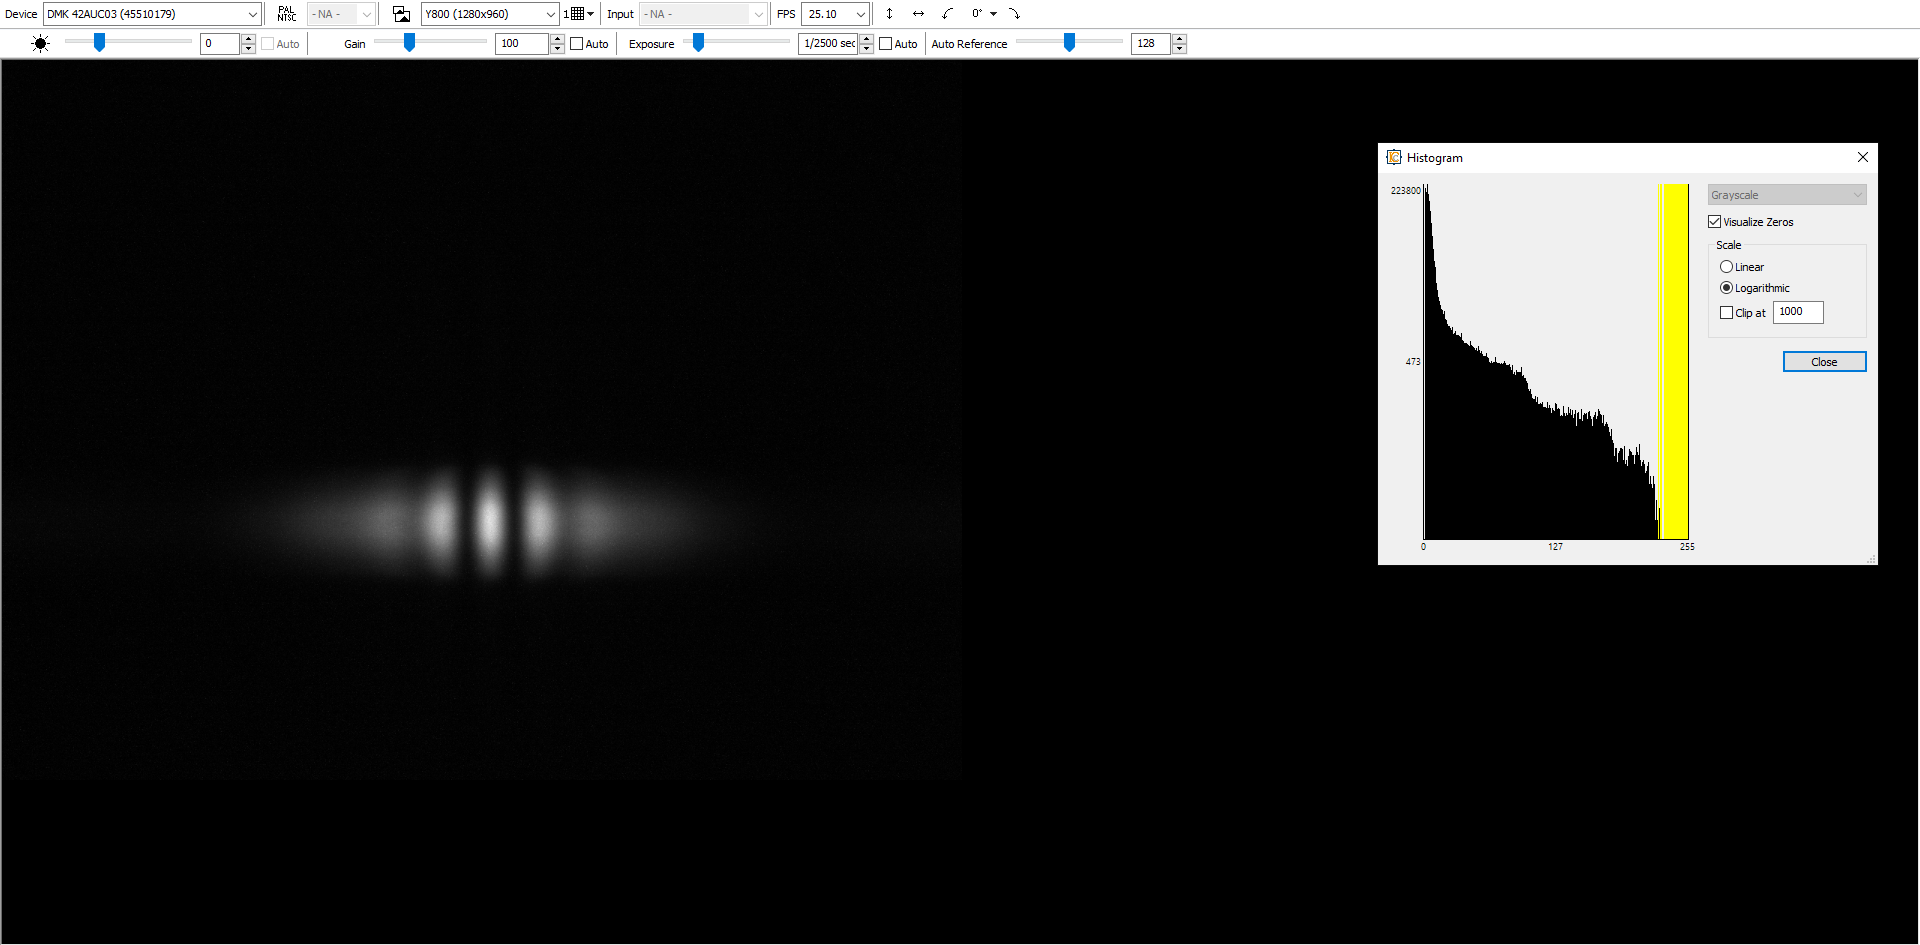
\includegraphics[width=\textwidth]{Interfero/Versuch2/ohnefilter}
		\captionof{figure}{Interferenzmuster bei einer Spaltbreite von
			\SI{0.200(5)}{mm} ohne Filter und einem Doppelspalt mit \SI{0.430(5)}{mm}}
		\label{fig:ohnefilter}
	\end{minipage}
\end{center}


\subsection{Bestimmung der Dicke einer Kunststoffschicht anhand des Interferenzmusters}

Für diesen Teil des Versuchs werden die Substratschicht, sowie die Polyacrylatschicht, in den Strahlengang geschoben. Dies ist in \autoref{fig:objekt} sichtbar.

\begin{center}
	\begin{minipage}[t]{0.5\textwidth}
		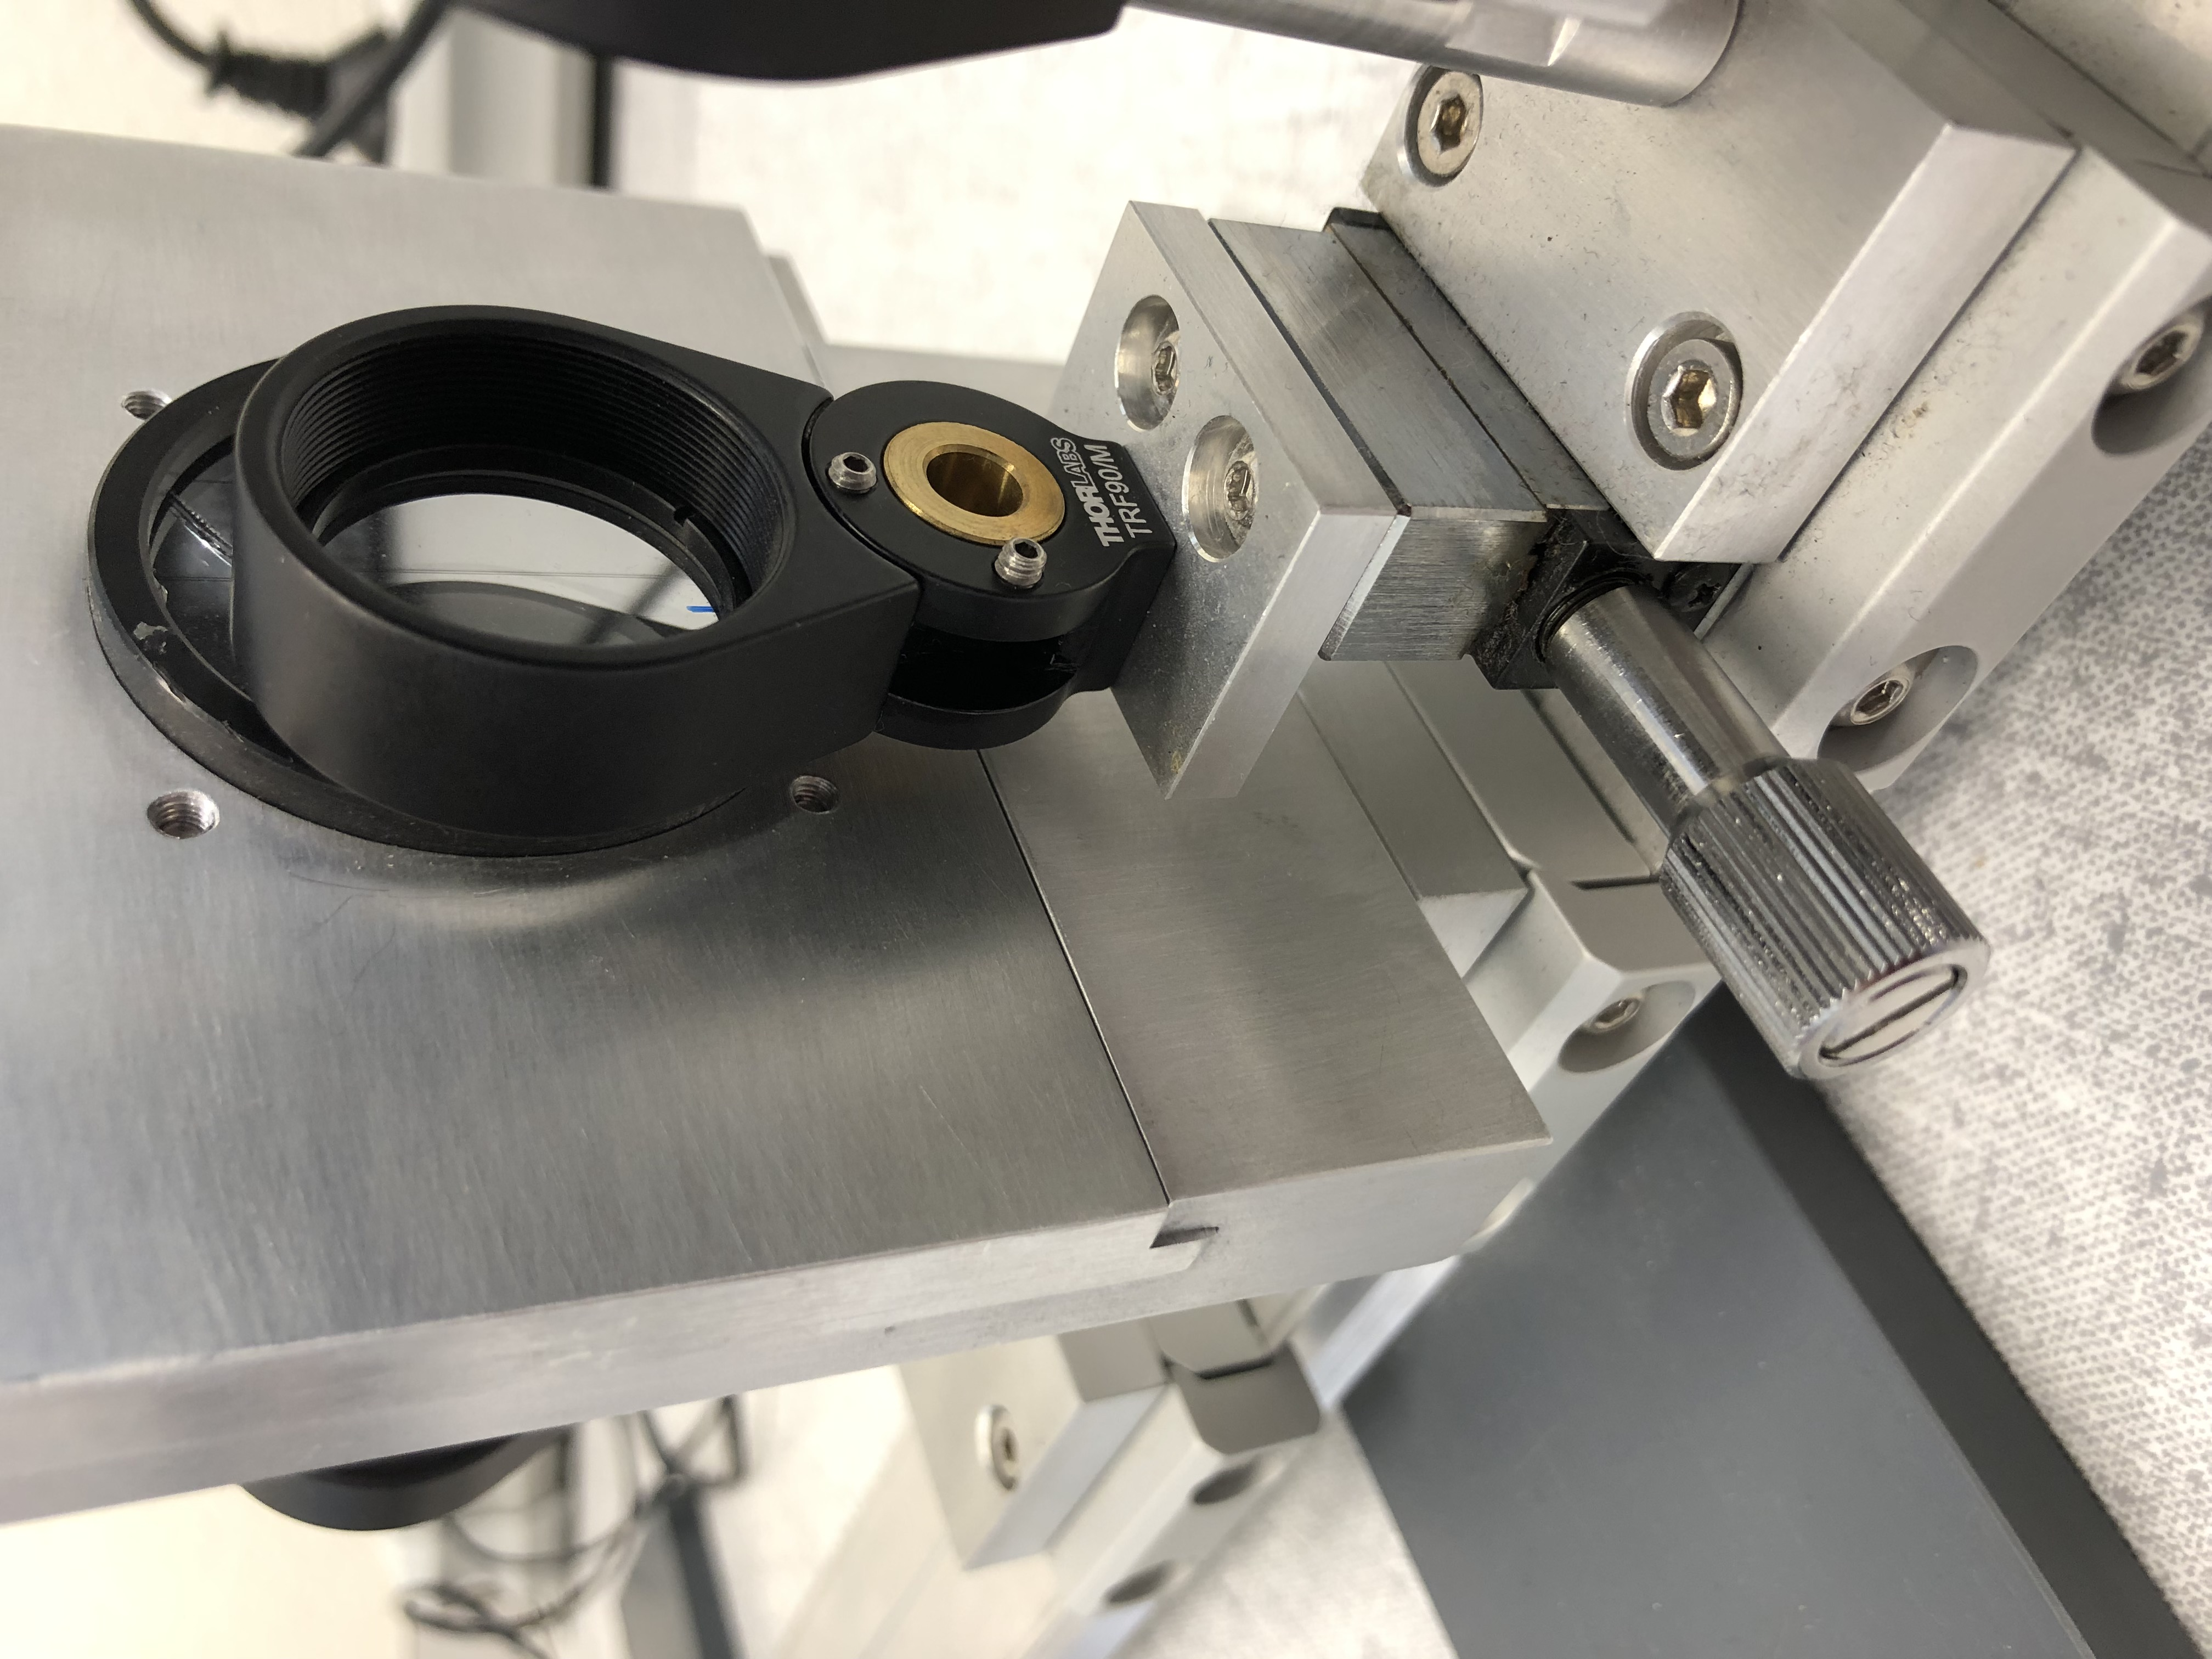
\includegraphics[angle=-90,width=\textwidth]{objekt}
		\captionof{figure}{in den Strahlengang geschobene Substratschicht, sowie die Polyacrylatschicht (bei blau markierten Strich) }
		\label{fig:objekt}
	\end{minipage}
\end{center}

\noindent Die Einstellungen für den Doppelspalt und den Spaltabstand wurden gleich gelassen, wie für Versuch 2, also ein Abstand des Doppelspalts von \SI{0.430(5)}{mm} und eine Spaltbreite von \SI{0.200(5)}{mm}, mit Berücksichtigung der Offsets. Weiters wird der Filter aus den Sthahlengang entferrnt, also das Filterrad in eine Position gedreht, sodass die Filter außerhalb sind.

\vspace{2mm}

\noindent Nun wird das Objekt mithilfe des Schraubmechanismus bewegt, bis ein leichter Sprung am aufgezeichneten Bild der Kamera sichtbar wird. Daran ist erkennbar, dass sich die Polyacrylatschicht nun vor einem der Doppelspalten befindet.

\vspace{2mm}

\noindent Nun werden die beiden entsprechenden Bilder aufgenommen, um so anhand der Verschiebung der Maxima auf die Dicke der Kunststoffschicht schließen zu können.

\begin{center}
	\begin{minipage}[t]{\textwidth}
		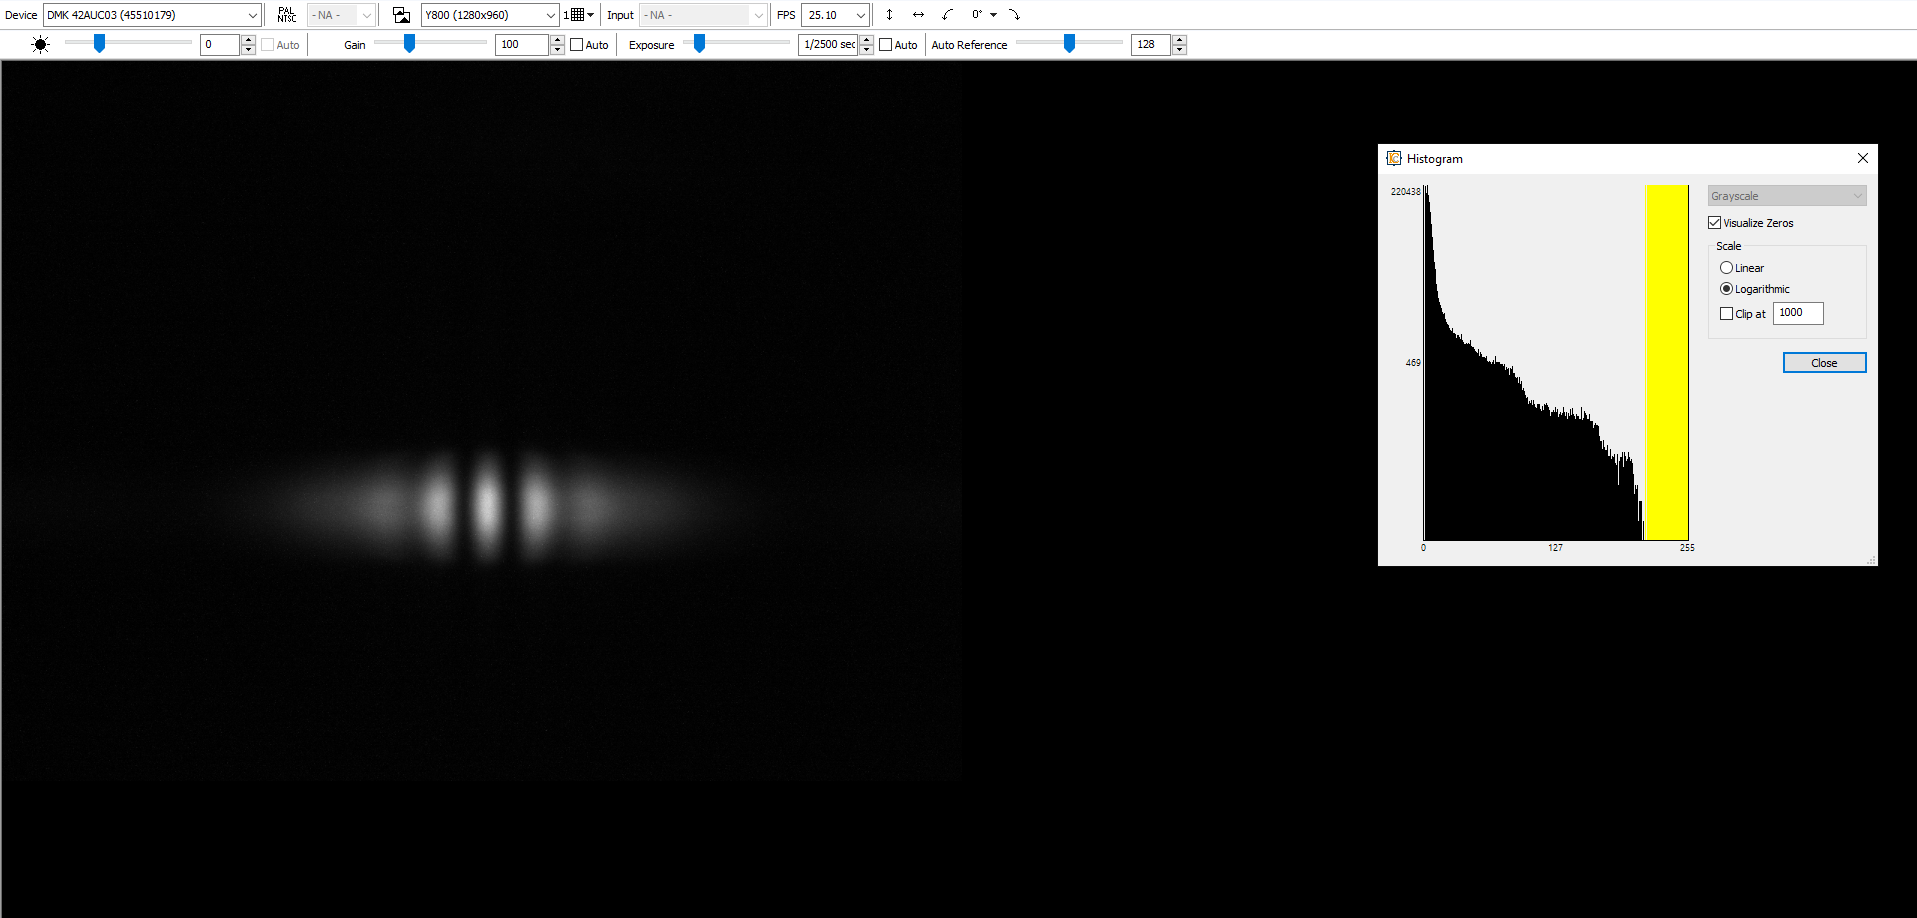
\includegraphics[width=\textwidth]{Interfero/Versuch3/schicht1}
		\captionof{figure}{Interferenzmuster mit der Substratschicht, bei einer Spaltbreite von \SI{0.200(5)}{mm} und einem Doppelspalt mit \SI{0.430(5)}{mm}}
		\label{fig:substrats}
	\end{minipage}
\end{center}

\begin{center}
	\begin{minipage}[t]{\textwidth}
		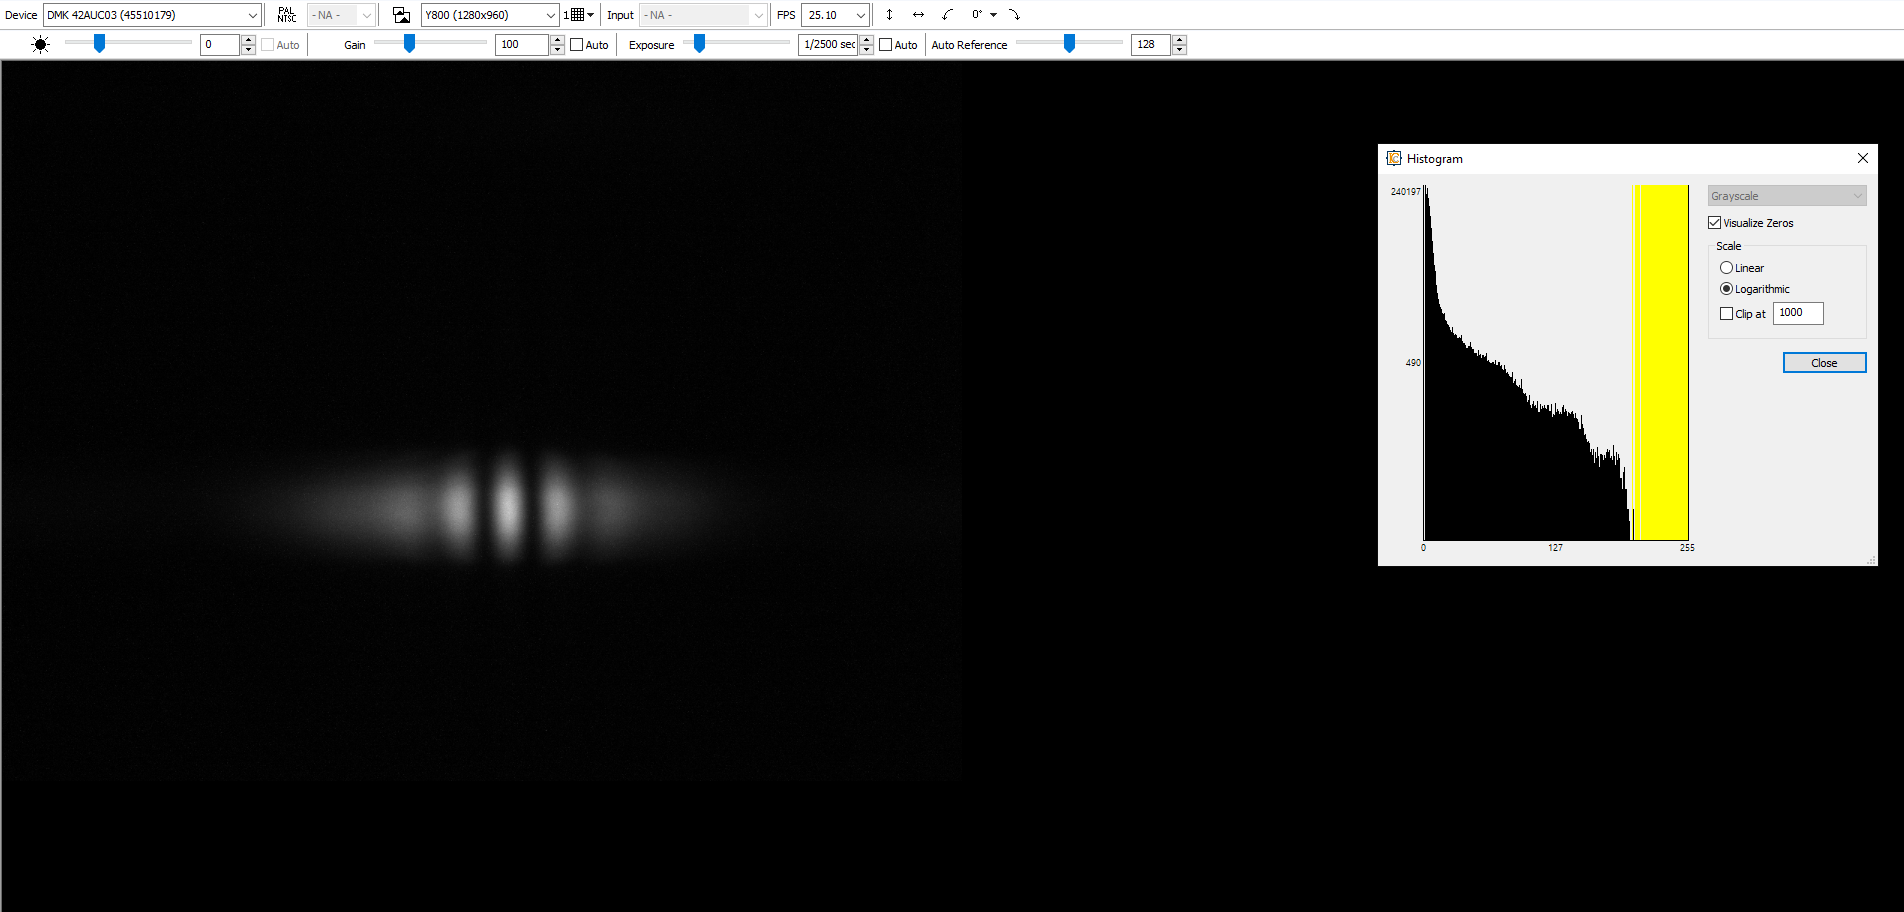
\includegraphics[width=\textwidth]{Interfero/Versuch3/sprungschicht}
		\captionof{figure}{Interferenzmuster mit der Substrat- und Polyacrylschicht, bei einer Spaltbreite von \SI{0.200(5)}{mm} und einem Doppelspalt mit \SI{0.430(5)}{mm}}
		\label{fig:polys}
	\end{minipage}
\end{center}

\noindent Die genaue Position der Maxima wird wieder, wie bereits unter Versuch 1 beschrieben, mithilfe der Bildbearbeitungssoftware ``imageJ`` ausgewertet und die so erhaltenen Daten in folgender Grafik veranschaulicht.

\begin{center}
	\begin{minipage}[t]{0.7\textwidth}
		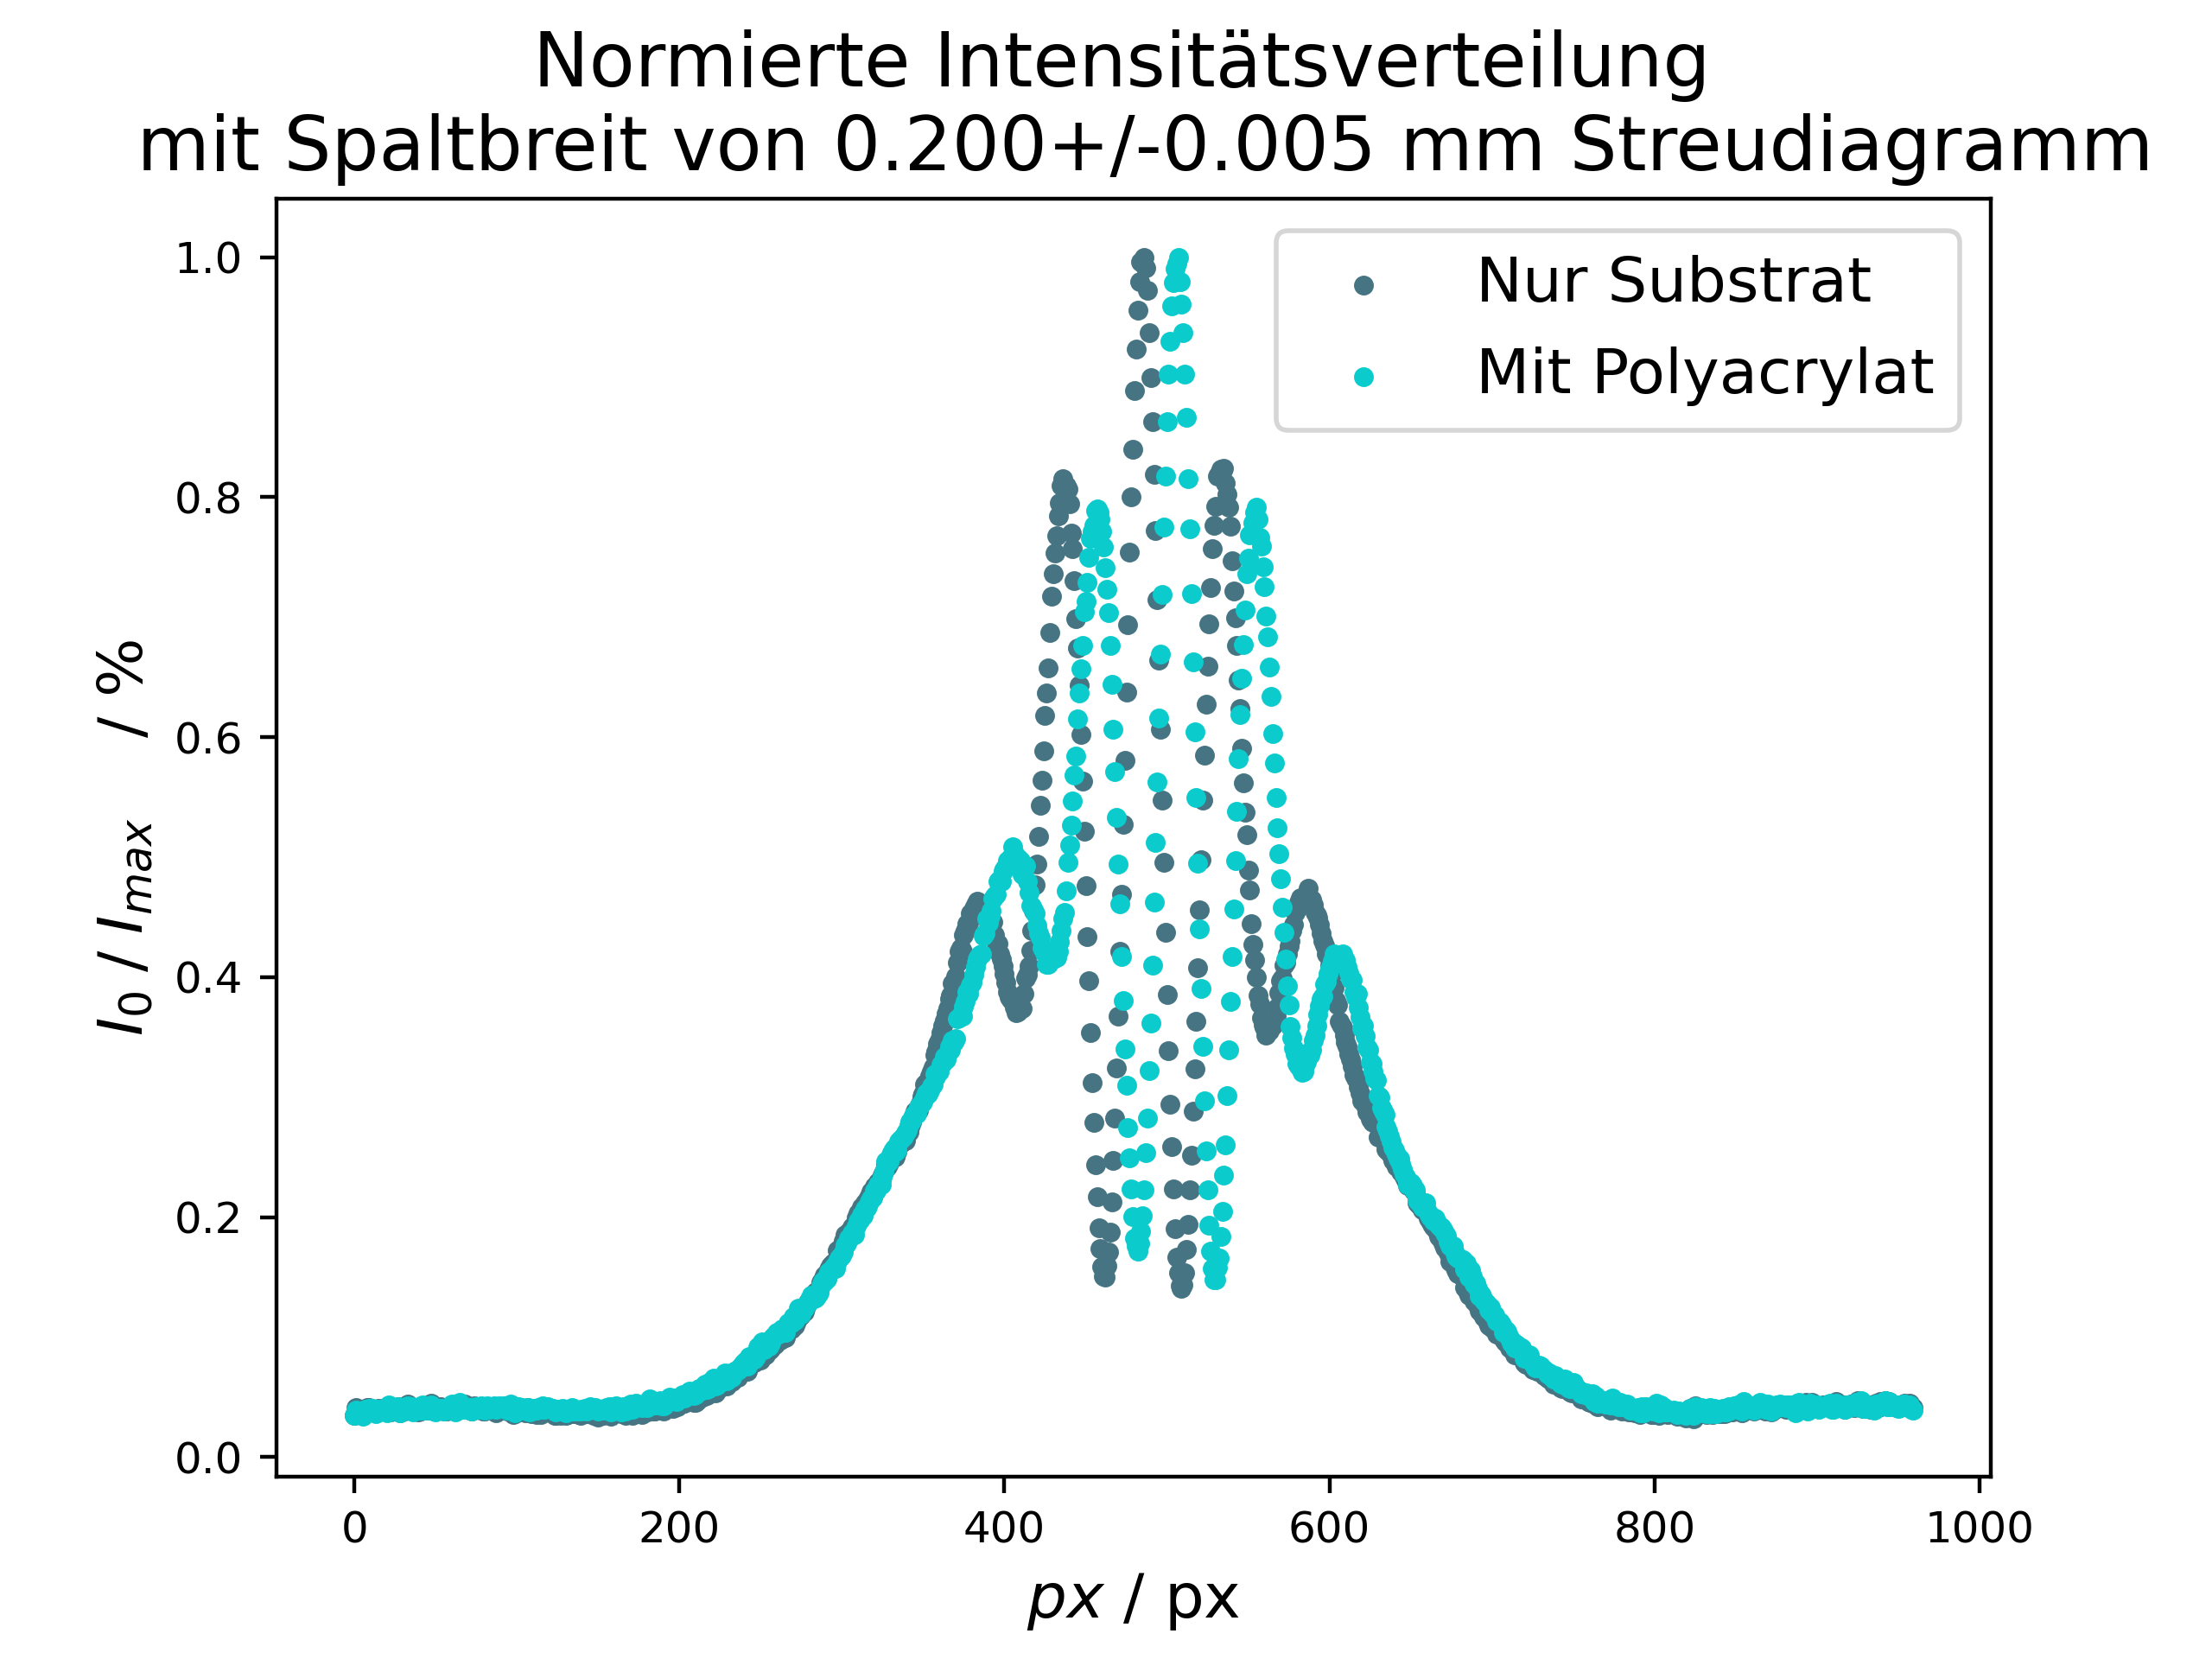
\includegraphics[width=\textwidth]{auswertung/sprung_gesamt}
		\captionof{figure}{Verteilung der Intensitätsmaxima auf die entsprechende Pixelzahl mit (türkis) und ohne (grau) Polyacrylschicht}
		\label{fig:sprung_ges}
	\end{minipage}
\end{center}



\subsection{Bestimmung der Größe einer Lichtquelle, bei der das Licht noch räumlich kohärent ist}

Für diesen Teil des Versuchs wird wieder der Bandpassfilter in den Strahlengang gedreht, um monochromatisches Licht zu erzeugen. Auch der Spaltabstand wird konstant bei \SI{0.200(5)}{mm}, unter der Berücksichtigung des Offsets, belassen.

\vspace{2mm}

\noindent Nun werden der Reihe nach unterschiedlich große Doppelspalte in den Aufbau geschoben und notiert, bei welchem Spaltabstand das erste Beugungsminimum sichtbar wird. Dies ist daran erkennbar, dass das Beugungsmuster verschwommen wird und die einzelnen Maxima nicht mehr unterscheidbar sind, wie beispielsweise für den Doppelspalt mit einem Abstand von \SI{0.230(5)}{mm} in \autoref{fig:v4} sichtbar.

\begin{center}
	\begin{minipage}[t]{\textwidth}
		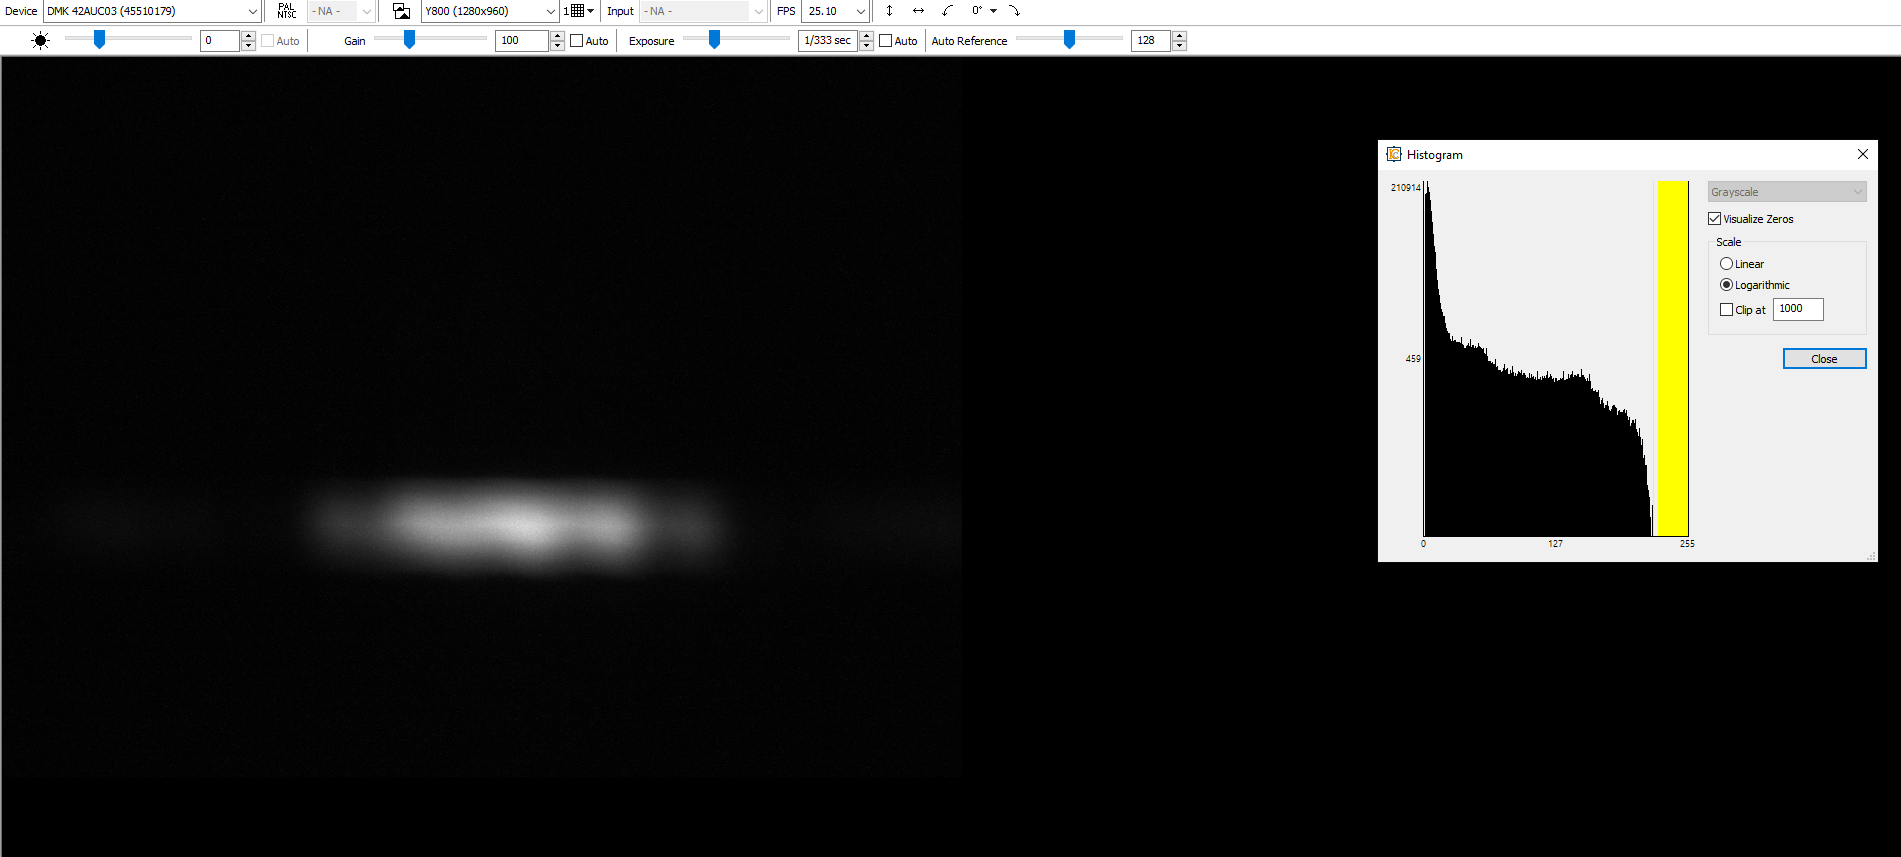
\includegraphics[width=\textwidth]{Interfero/Versuch4/mittelkontrastmin}
		\captionof{figure}{Interferenzmuster des ersten Minimums bei einer Spaltbreite von \SI{0.200(5)}{mm} und einem Doppelspalt mit \SI{0.230(5)}{mm}}
		\label{fig:v4}
	\end{minipage}
\end{center}

\noindent Da der genaue Punkt des Minimums sehr schwer zu finden ist, wurde der
Spalt immer geschlossen und langsam wieder geöffnet, bis das von der
Computersoftware aufgezeichnete Bild das erste Mal einen Verschwommenen
Eindruck macht. Um den statistischen Fehler dieser subjektiven Wahrnehmung
möglichst gering zu halten wurde dieser Vorgang von den Experimentatoren
abwechselnd 10 mal wiederholt. Die erhaltenen Werte sind in folgender \autoref{tab:spalte}
aufgelistet. Bei den Werten ist dabei zu beachten, dass diese direkt von der
Mikrometerschraube abgelesen wurden und daher noch der Offset von
\SI{0.210(5)}{mm} addiert werden muss.

\begin{table}
	\caption{Abgelesene Werte für die Spaltbreite bei der das erste
		Minimum sichtbar ist \\ d \dots Größe des Doppelspalts}
	\begin{center}
		\begin{tabular}{|c|c|c|} \hline
			\textbf{d = \SI{0.430(5)}{mm}} & \textbf{ d = \SI{0.230(5)}{mm}} & \textbf{d = \SI{0.130(5)}{mm}} \\ \hline
			0.410                          & 0.800                           & 1.680                          \\
			0.380                          & 0.780                           & 1.460                          \\
			0.390                          & 0.760                           & 1.510                          \\
			0.360                          & 0.800                           & 1.730                          \\
			0.380                          & 0.750                           & 1.530                          \\
			0.370                          & 0.810                           & 1.420                          \\
			0.410                          & 0.790                           & 1.480                          \\
			0.390                          & 0.750                           & 1.340                          \\
			0.410                          & 0.770                           & 1.260                          \\
			0.400                          & 0.760                           & 1.270                          \\ \hline
		\end{tabular}
	\end{center}
	\label{tab:spalte}
\end{table}









\section{Auswertung}

\noindent Um zu sehen wie sich die Unsicherheit der Messungen bis in die Ergebnisse
fortpflanzt, ist \autoref{eq:Unsicherheitsfortpflanzung} verwendet worden.
Die Grundlagen dieser Gleichung stammen von den Powerpointfolien von
GUM.\cite{WolfgangKessel2004} Die Verallgemeinerung ist von Wikipedia entnommen
worden \cite{2020Fehler}.
Für die Auswertung ist die Progammiersprache Python im speziellen das
Packet \verb#scipy#, zur Hilfe genommen worden.

\begin{equation}
	\label{eq:Unsicherheitsfortpflanzung}
	V_y = J(x) \cdot V_x \cdot J^{T}(x)
\end{equation}

\noindent Wobei $V_y$ und $V_x$ die Kovarianzmatrizen von den Vektoren $\bm{y}$ und $\bm{x}$ sind.
$\bm{x}$ ist der Vektor der Eingangsvariablen und $\bm{y}$ ist der Vektor der Ausgangsvariablen.
$J$ ist die Jakobimatrix der vektorwertigen Funktion $\bm{y} = \vec{F}(\bm{x})$.
So lassen sich die Komponenten der Matrix relativ einfach anschreiben $J_{ij}(x) = \frac{\partial{y_i}}{\partial{x_j}}(x)$.
Damit man die Unsicherheit der einzelnen Variablen $y_i$ bekommt, muss nur die Quadratwurzel des i-ten Diagonalelementes der
$\bm{y}$-Kovarianzmatrix genommen werden $u_i= \sqrt{\mathrm{diag}(V_y)_i}$.
Da in diesem Experiment meistens nur skalare Funktionen untersucht werden, vereinfacht
sich die \autoref{eq:Unsicherheitsfortpflanzung} dramatisch und die Unsicherheit
der Variable $y$ lässt sich einfach so berechnen:

\begin{equation}
	\label{eq:graduncentainty}
	u_y = \sqrt{\mathrm{grad} y^T \cdot V_x \cdot \mathrm{grad} y}
\end{equation}

\subsection{Einfluss der Größe einer Lichtquelle auf das Interferenzmuster eines Doppelspalts}

Die gemessenen Daten der bestimmten Maximal und Minimalitensitäten werden nun, unter
Verwendung von \autoref{eq:kontrast} geplottet, was in folgender \autoref{fig:kontrast}
sichtbar ist. Zusätzlich wird noch der theoretische Verlauf unter Verwendung
von \autoref{eq:kontrast} (rechter Teil) eingezeichnet.

\begin{figure}[H]
	\begin{center}
		\begin{minipage}[t]{0.7\textwidth}
			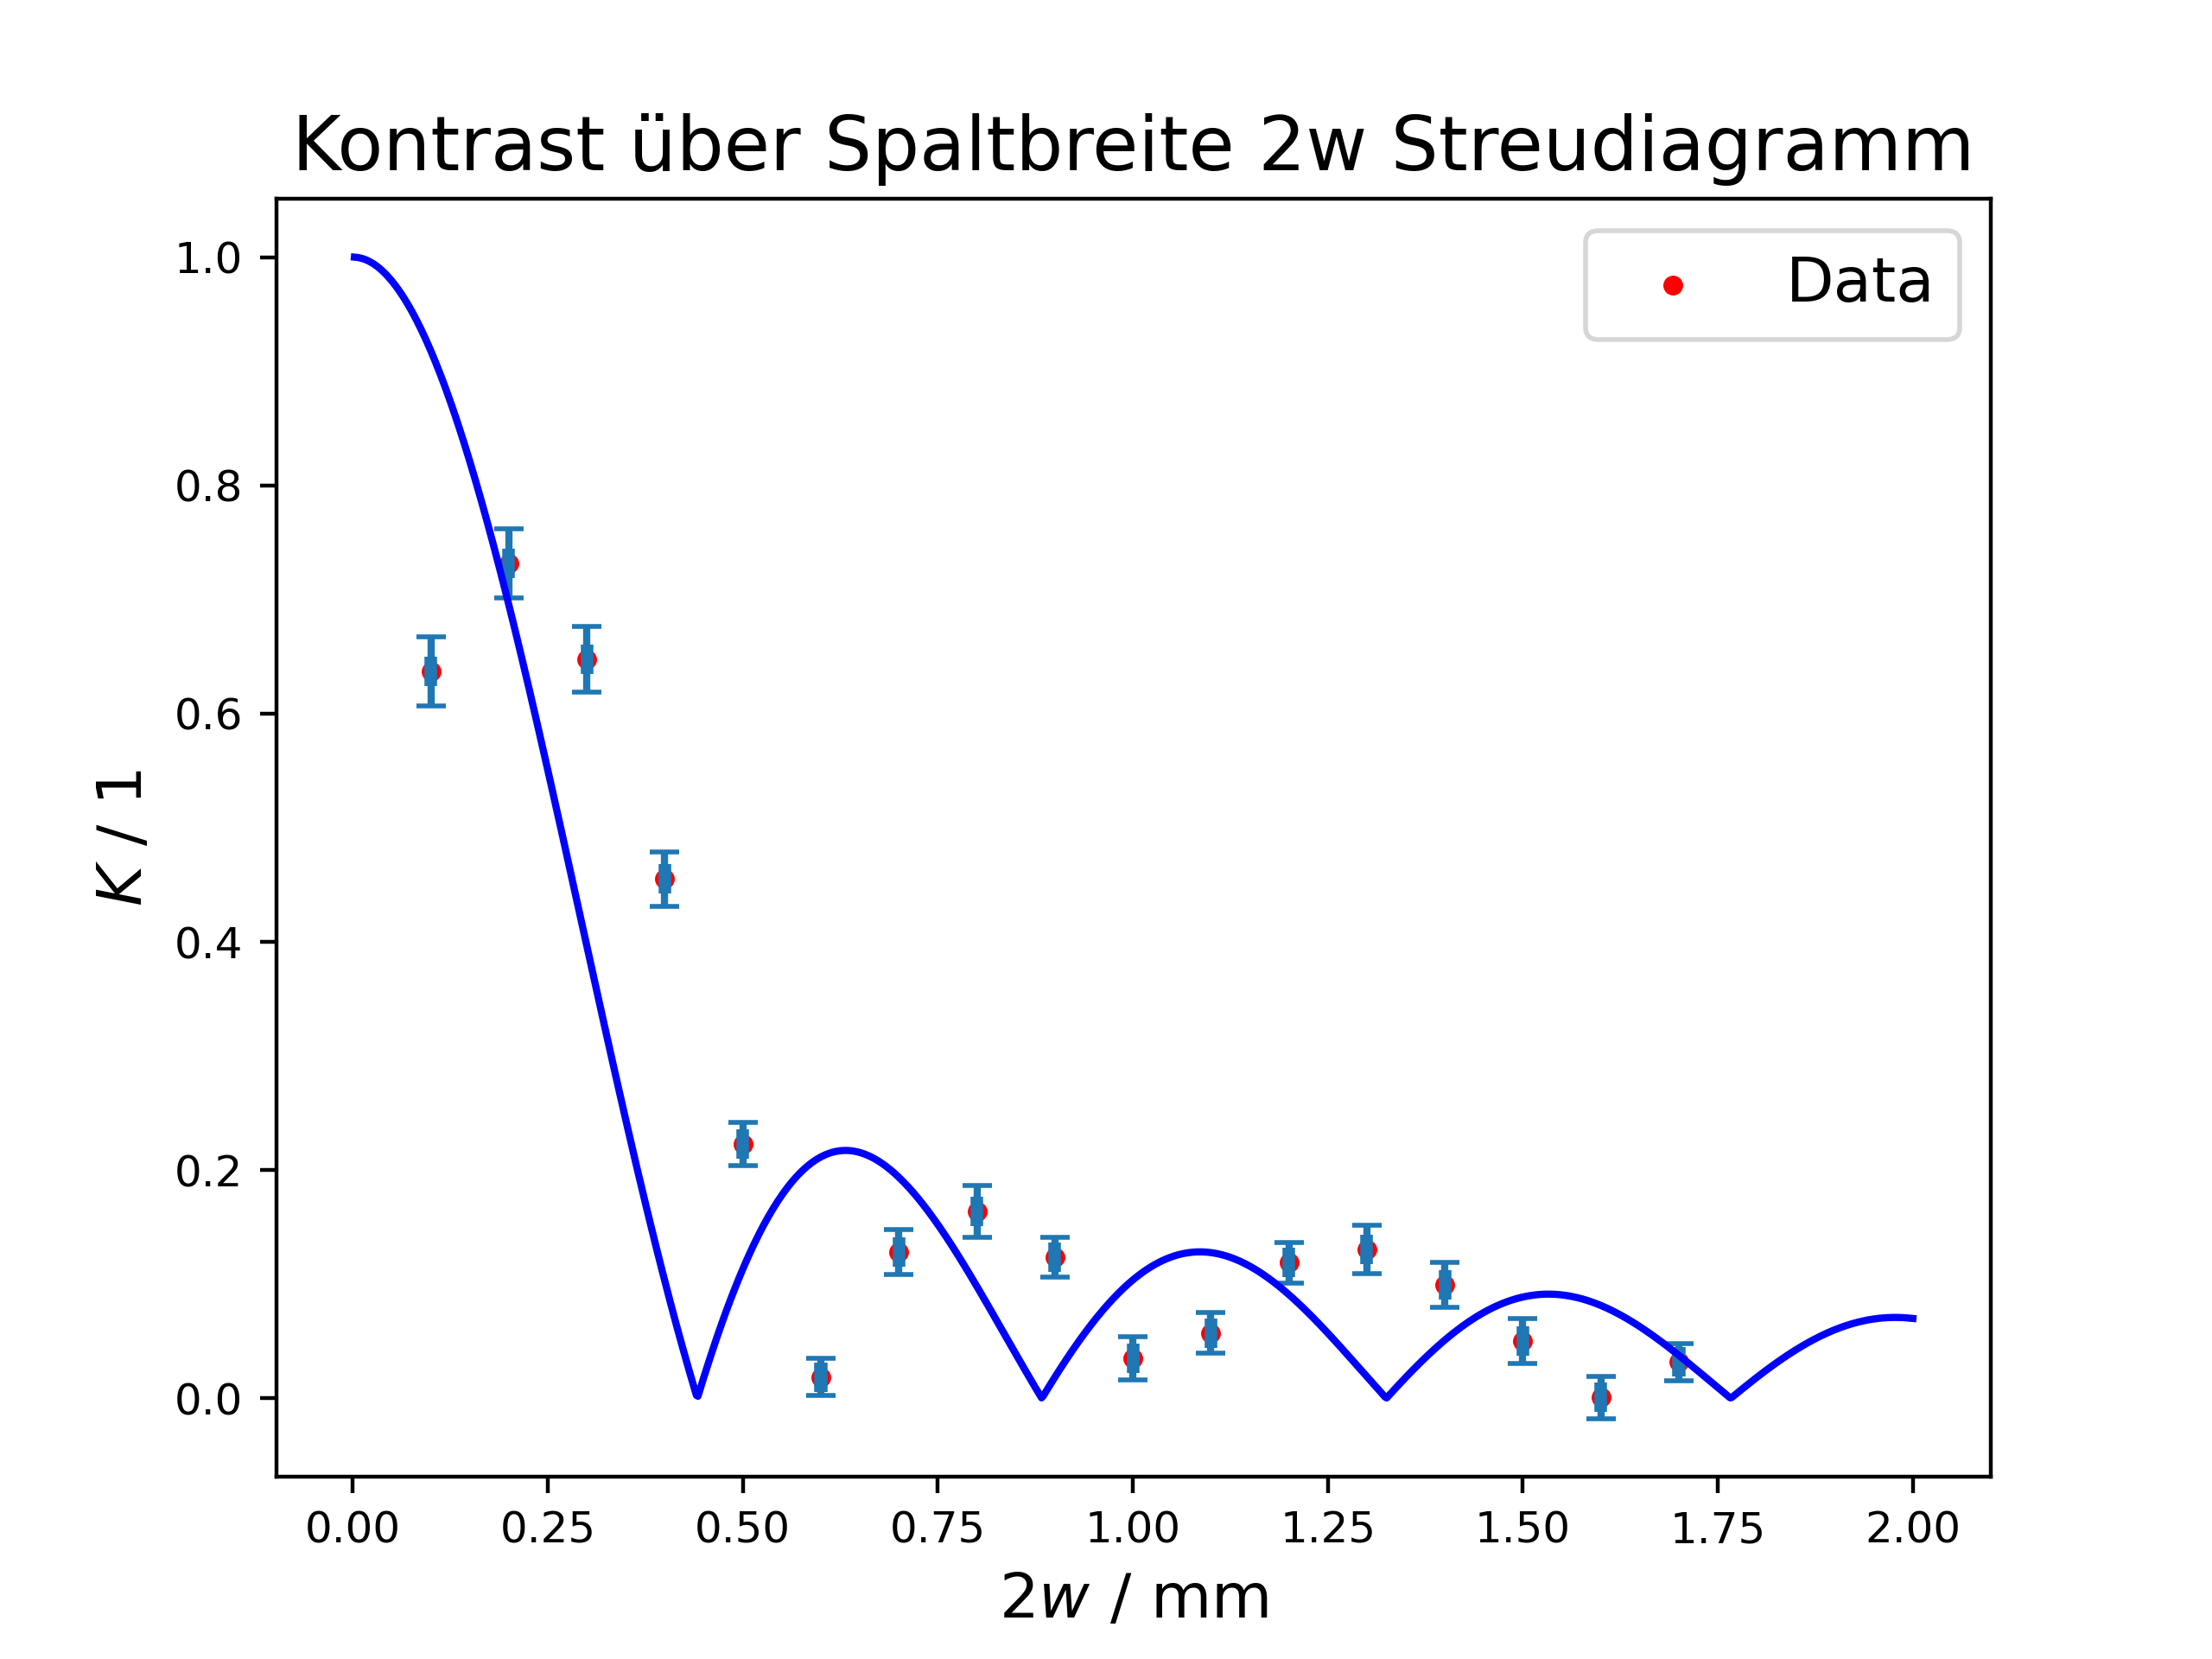
\includegraphics[width=\textwidth]{auswertung/kontrast}
		\end{minipage}
	\end{center}
	\caption{Kontrast des Beugungsmusters mit theoretischen Fit und gemessenen Werten}
	\label{fig:kontrast}
\end{figure}





\subsection{Einfluss der spektralen Breite einer Lichtquelle auf das Interferenzmuster eines Doppelspalts}

Um einen direkten Vergleich der Interferenzmuster aus \autoref{fig:bandpassfilter}, \autoref{fig:langpassfilter} und \autoref{fig:ohnefilter} zu ermöglichen, wurden die Entsprechenden Interferenzmuster nochmals extra als Großaufnahme abgebildet.

\begin{center}
	\begin{minipage}[t]{\textwidth}
		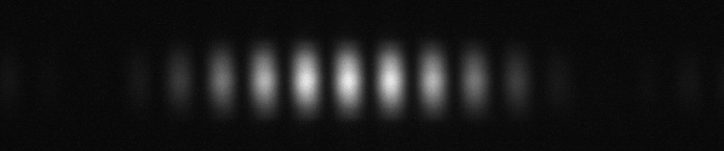
\includegraphics[width=\textwidth]{Interfero/Versuch2/bandpassfilter_m}
		\captionof{figure}{Interferenzmuster bei einer Spaltbreite von \SI{0.200(5)}{mm} unter Verwendung des Bandpassfilters und einem Doppelspalt mit \SI{0.430(5)}{mm}}
		\label{fig:bandpassfilter_m}
	\end{minipage}
\end{center}

\begin{center}
	\begin{minipage}[t]{\textwidth}
		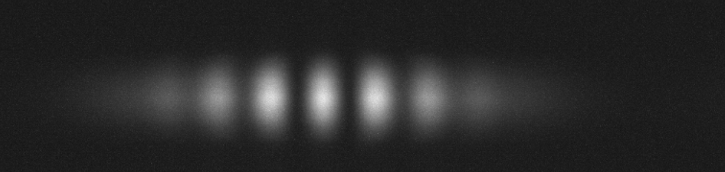
\includegraphics[width=\textwidth]{Interfero/Versuch2/langpassfilter_m}
		\captionof{figure}{Interferenzmuster bei einer Spaltbreite von \SI{0.200(5)}{mm} unter Verwendung des Langpassfilters und einem Doppelspalt mit \SI{0.430(5)}{mm}}
		\label{fig:langpassfilter_m}
	\end{minipage}
\end{center}

\begin{center}
	\begin{minipage}[t]{\textwidth}
		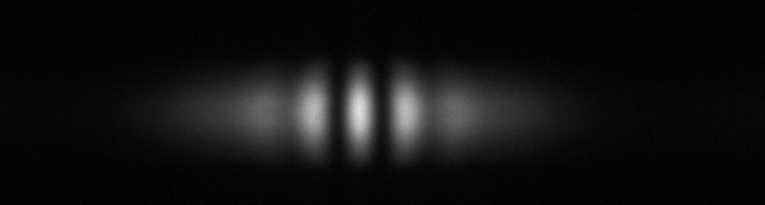
\includegraphics[width=\textwidth]{Interfero/Versuch2/ohnefilter_m}
		\captionof{figure}{Interferenzmuster bei einer Spaltbreite von \SI{0.200(5)}{mm} ohne Filter und einem Doppelspalt mit \SI{0.430(5)}{mm}}
		\label{fig:ohnefilter_m}
	\end{minipage}
\end{center}

\noindent Dieser Vergleich zeigt klar, dass bei einer geringeren durchgelassenen Wellenlänge die Auflösung des Bildes deutlich besser ist.


\subsection{Bestimmung der Dicke einer Kunststoffschicht anhand des Interferenzmusters}

Um die Verschiebung der Maxima durch die Polyacrylatschicht genauer
festzustellen, wurde der Pixelbereich des Graphen aus \autoref{fig:sprung_ges}
vergrößert in folgender \autoref{fig:sprung} dargestellt, um den relevanten
Bereich besser darzustellen.

\begin{center}
	\begin{minipage}[t]{0.7\textwidth}
		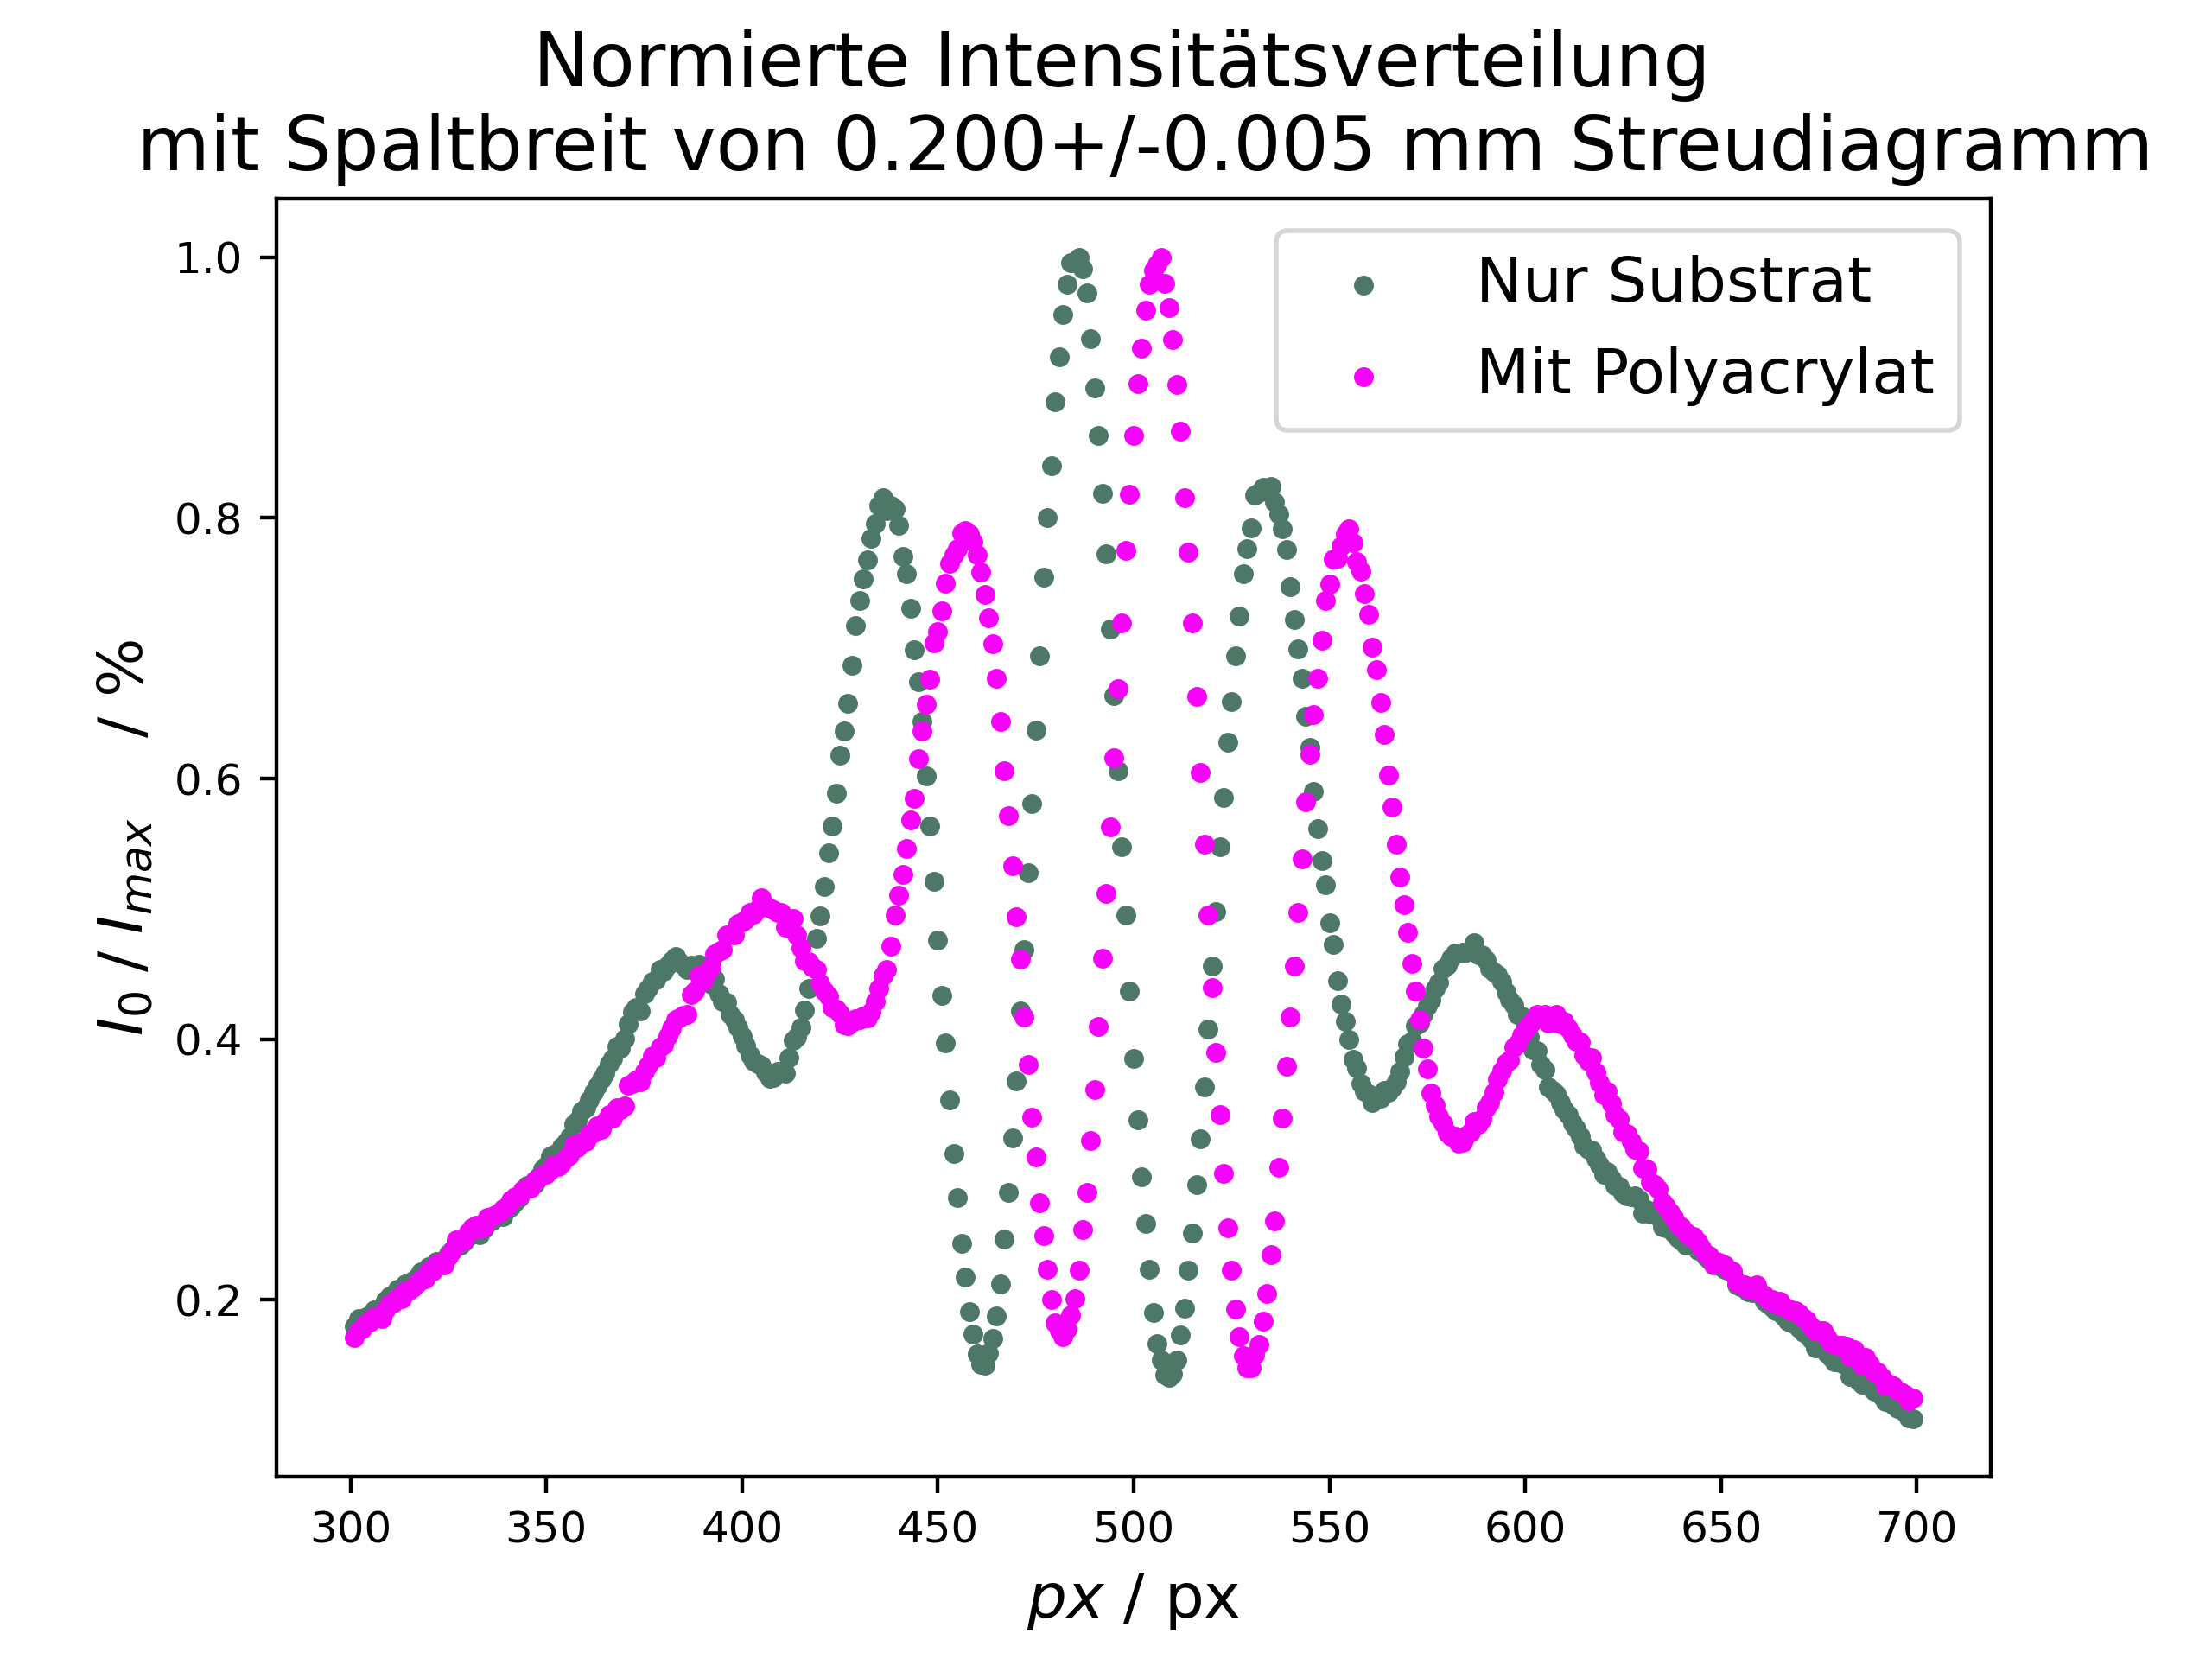
\includegraphics[width=\textwidth]{auswertung/sprung}
		\captionof{figure}{Verteilung der Intensitätsmaxima auf die entsprechende Pixelzahl mit (pink) und ohne (dunkelgrün) Polyacrylatschicht }
		\label{fig:sprung}
	\end{minipage}
\end{center}

\noindent Datenpunkte der zwei äußersten Peaks wurden verwendet um die Nanometer pro
Pixelzahl zu bestimmen. Die zwei Peaks sind 4 Wellenlängen von einander
entfernt, da jeder Peak eine Wellenlängen zum Nächsten hat, dies ist anhand
\autoref{eq:wegunterschied} erkennbar.

\begin{equation}
	M = \frac{4\lambda}{P_L-P_R} = \frac{4 \cdot \num{633(5)}}{\num{587(1)}-\num{383(1)}} = \SI{1.24(16)}{\nm\per\px}
	\label{eq:nmperpx}
\end{equation}


\noindent Da wir nun ein Maß besitzen um Pixel in Nanometer umzurechnen ist es möglich den
den Versatz der 0. Ordnung $\Delta P_0$ in \si{\nm} umzurechnen.

\begin{equation}
	\Delta s = \Delta P_0 \cdot M = \num{507(1)}-\num{486(1)} \cdot \num{1.24(16)} \si{\nm} = \SI{260(30)}{\nm}
	\label{eq:peakversatz}
\end{equation}

\noindent Mit diesem Versatz und dem Brechungsindex von Polyacrylat $n_P = 1.492 @
	\SI{633}{\nm}$ \cite{vorlageinterfero} und Luft $n_L \approx 1$ kann mit
\autoref{eq:dicke} die Dicke $t$ der Polyacrylschickt bestimmt werden. Da es
sich um die 0. Ordnung handelt ist $m=0$ und somit erhält man:
\begin{equation}
	t = |\frac{\Delta s}{n_P-n_L}| = \SI{530(70)}{\nm}
	\label{eq:dickederschicht}
\end{equation}


%Rechnung



\subsection{Bestimmung der Größe einer Lichtquelle, bei der das Licht noch räumlich kohärent ist}

Zunächst wurden der Mittelwert und die Standardabweichung der gemessenen Werte aus \autoref{tab:spalte} bestimmt, was in folgender Tabelle sichtbar ist.

\begin{table}[H]
	\captionof{table}{Mittelwert und Standardabweichung der Werte für die
		Spaltbreite bei der das erste Minimum sichtbar ist \\ $d \dots$ Größe des
		Doppelspalts \\ $\overline{2w} \dots$ errechneter Mittelwert \\ $\Delta \dots$
		entsprechende Unsicherheit}
	\begin{center}
		\begin{tabular}{|c|c|c|c|} \hline
			{}              & \textbf{ d = \SI{0.430(5)}{mm}} & \textbf{ d = \SI{0.230(5)}{mm}} & \textbf{d = \SI{0.130(5)}{mm}} \\ \hline
			$\overline{2w}$ & 0.390                           & 0.777                           & 1.49                           \\
			$\Delta$        & 0.006                           & 0.007                           & 0.05                           \\ \hline
		\end{tabular}
	\end{center}
\end{table}


\noindent Anhand dieser Daten wurde folgende Grafik geplottet.

\begin{center}
	\begin{minipage}[t]{0.7\textwidth}
		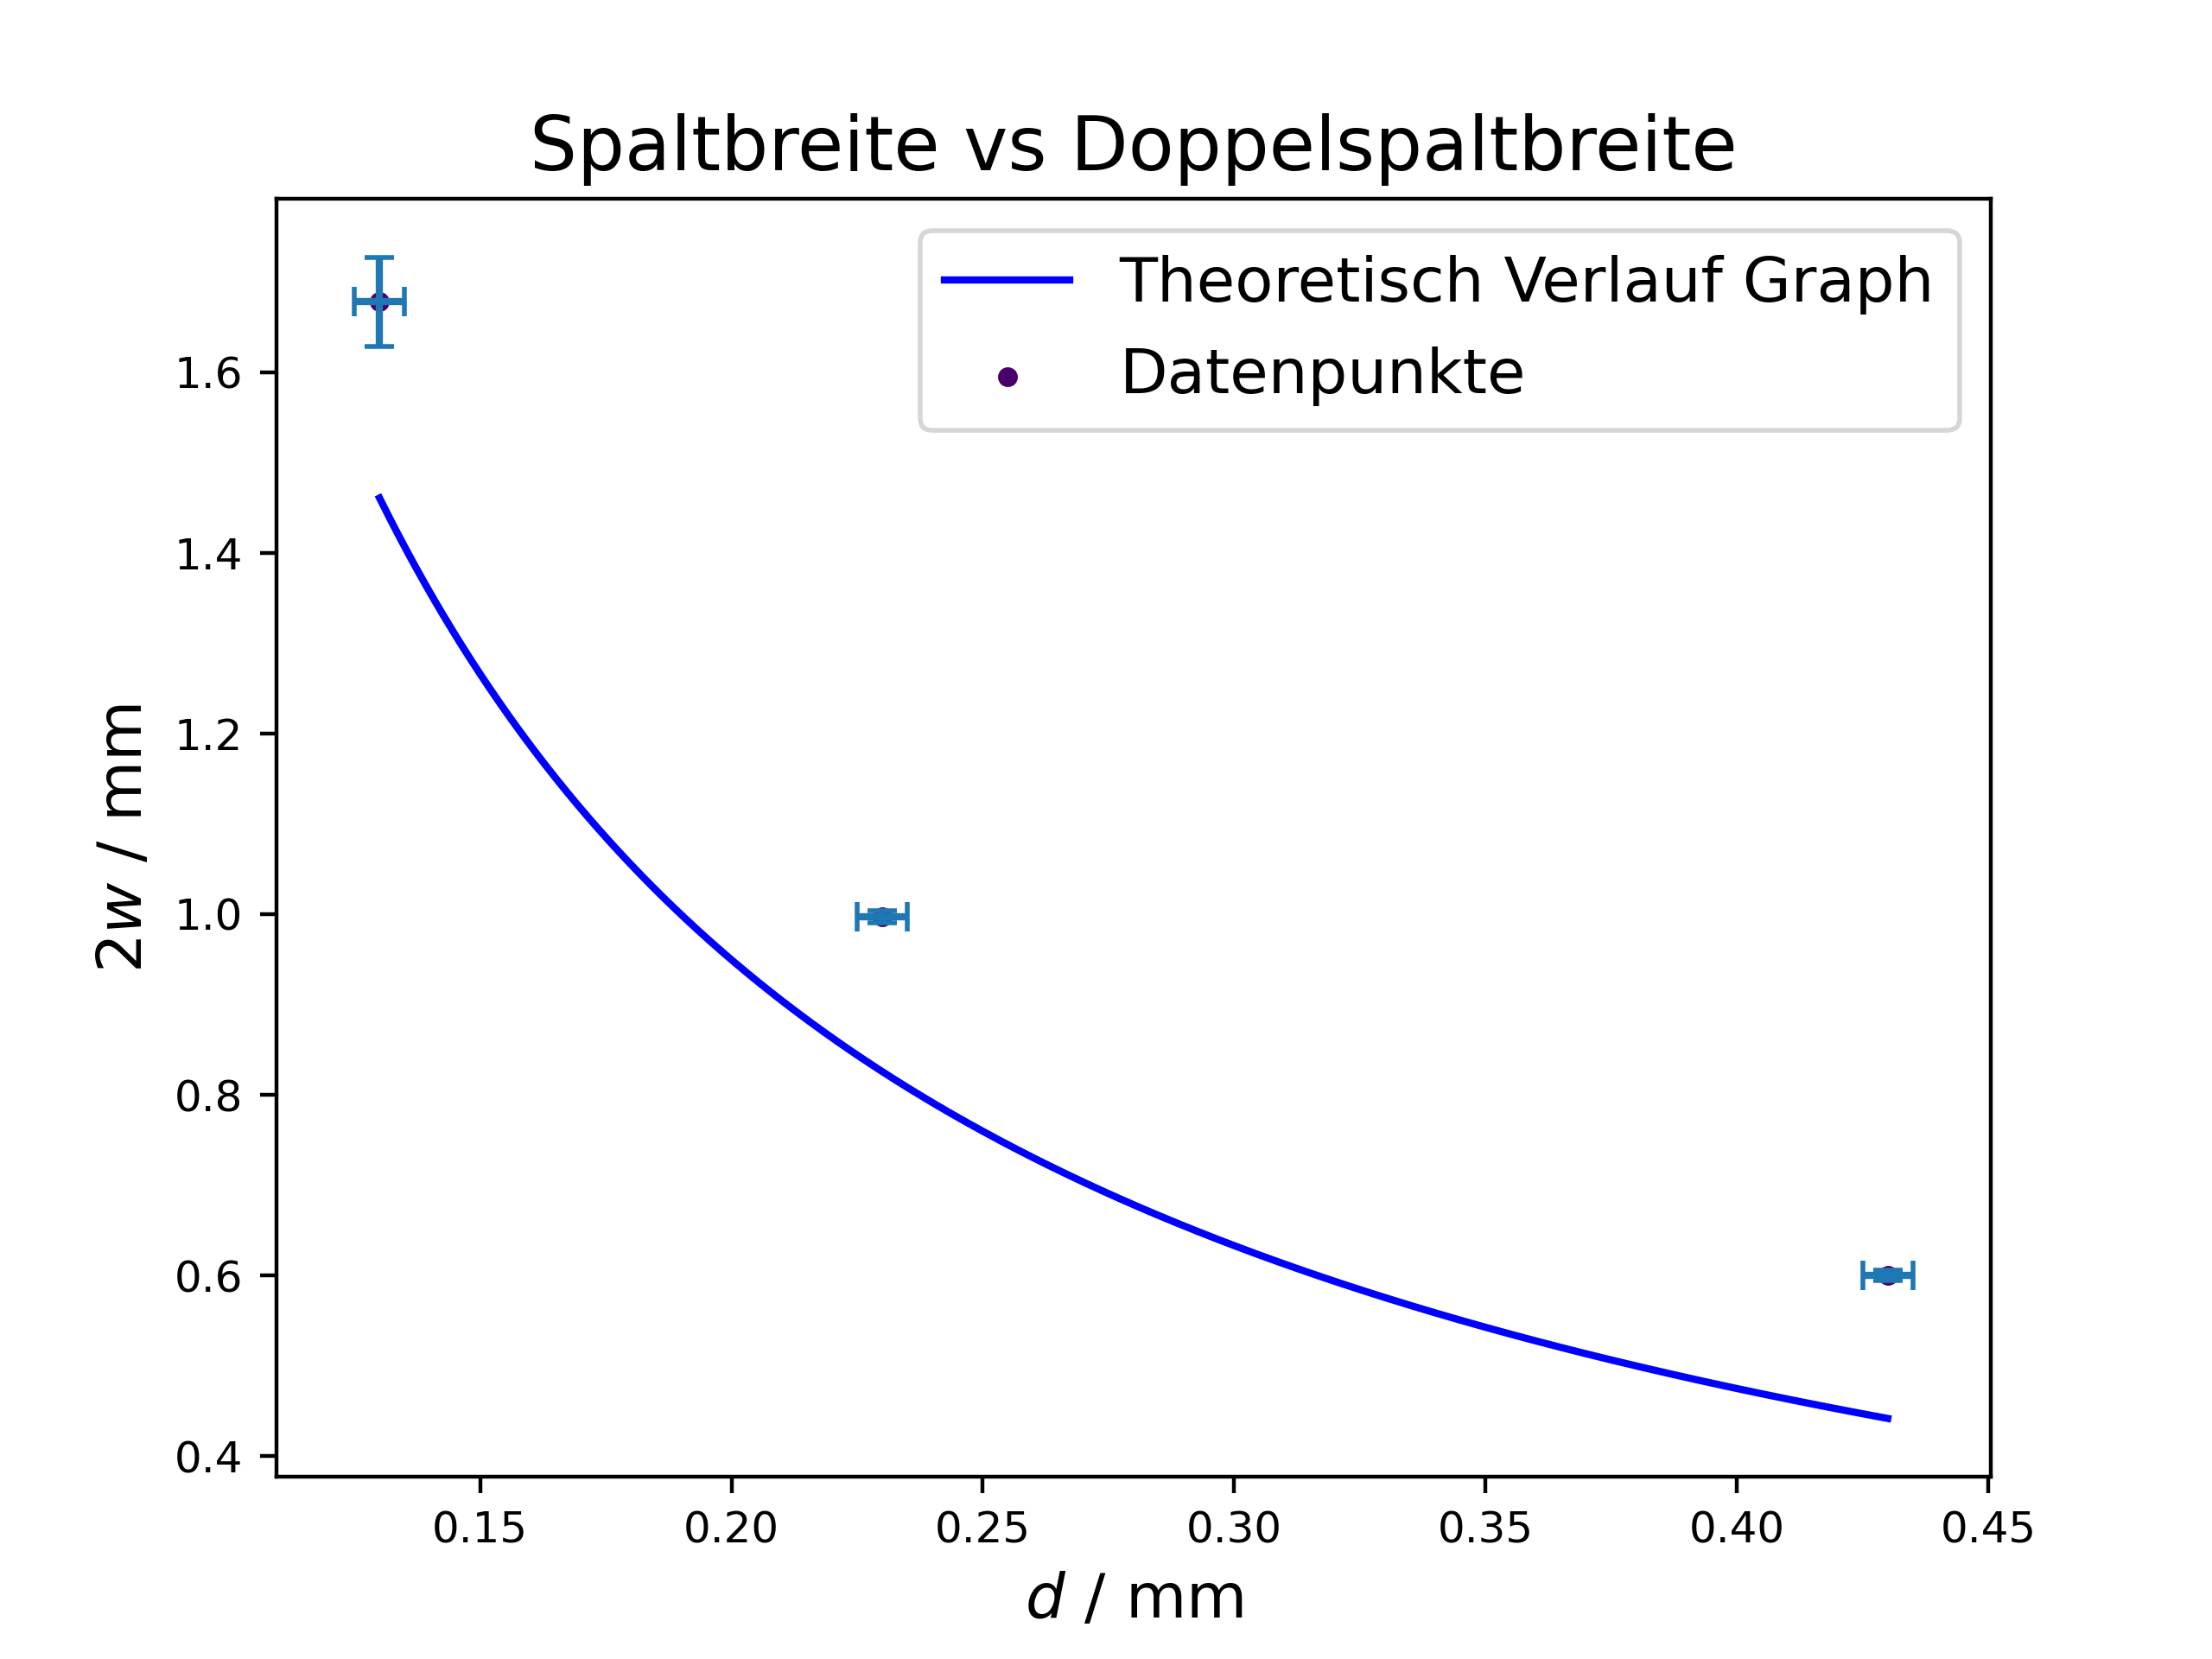
\includegraphics[width=\textwidth]{spaltvsdpspalt}
		\captionof{figure}{Spaltbreite beim ersten Kontrastminimum aufgetragen zur Doppelspaltbreite}
		\label{fig:spaltvsdpspalt}
	\end{minipage}
\end{center}


\section{Diskussion}\label{disk}

\subsection{Einfluss der Größe einer Lichtquelle auf das Interferenzmuster
	eines Doppelspalts}

Vergleicht man die gemessenen Werte mit dem theoretischen Verlauf der Kurve,
fällt sofort auf, dass diese um einen bestimmten Faktor verschoben scheinen. Es
könnte sich dabei um einen systematischen Fehler handeln.

\noindent Der erste aufgezeichnete Punkt weicht besonders stark von der theoretischen
Kurve ab. Betrachtet man das zugehörige Foto, siehe
\autoref{fig:vergleichgrau}, stellt man fest, dass der Hintergrund des Bildes
etwas gräulicher als die anderen ist, wodurch sich der Kontrast der weißen
Maxima klarerweise ändert, wie auch in den Daten ersichtlich, siehe \autoref{fig:ausreisergraph}.

\begin{figure}[H]
	\begin{center}
		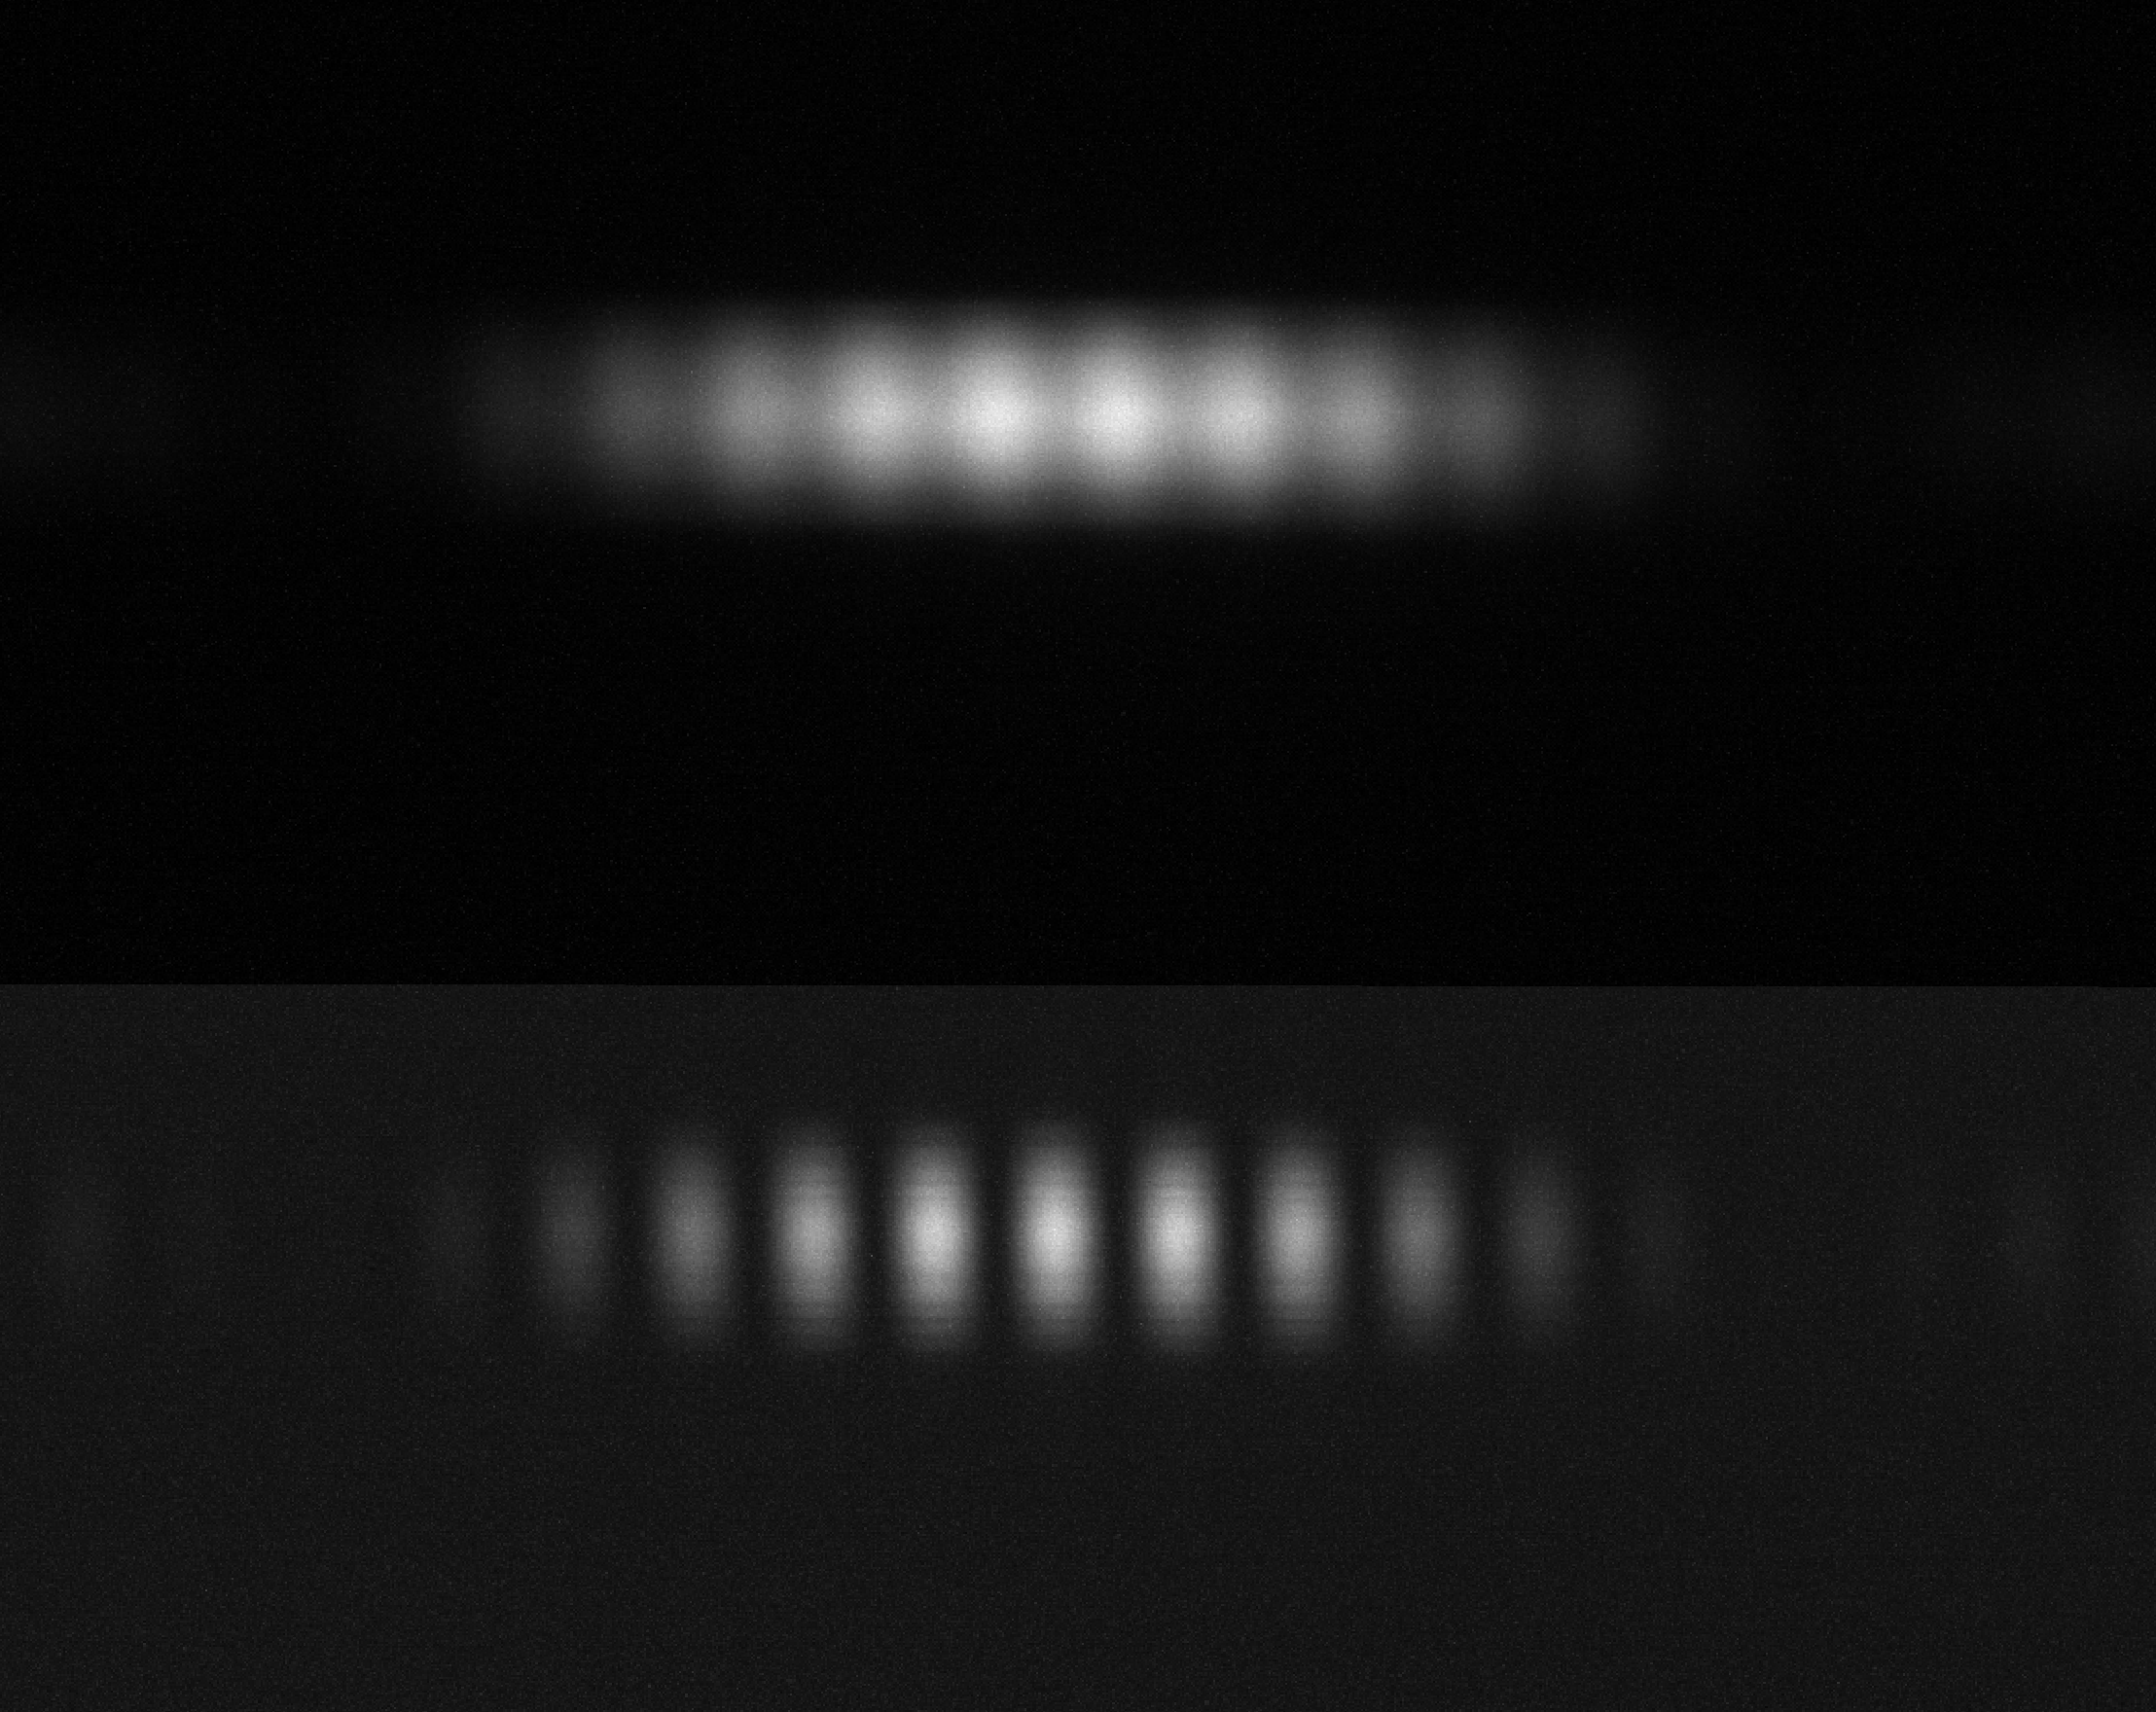
\includegraphics[width=0.95\textwidth]{./Interfero/Versuch1/vergleich.png}
	\end{center}
	\caption{Unten sieht man, dass das Hintergrundschwarz, bei
		einer Spaltöffnung von \SI{0.1}{\mm} gräulicher ist als bei den anderen
		Spaltöffnungen zb. bei \SI{0.8}{\mm} Oben, ersichtlich}
	\label{fig:vergleichgrau}
\end{figure}



\subsection{Einfluss der spektralen Breite einer Lichtquelle auf das Interferenzmuster eines Doppelspalts}

Wie es die Theorie voraussagt, sind die Bilder (\ref{fig:bandpassfilter_m}
\ref{fig:langpassfilter_m} \ref{fig:ohnefilter_m}) deutlich verschwommener, wenn
mehrere unterschiedliche Wellenlängen durchgelassen werden, die zeitliche
Kohärenz also erhöht wird.

\subsection{Bestimmung der Dicke einer Kunststoffschicht anhand des Interferenzmusters}

Der erhaltene Wert für die Dicke der Kunststoffschicht liegt in einer zu
erwartenden Größenordnung. Allerdings liegen hierzu keine genauen Angaben vor,
wodurch keine qualitative Aussage über das erhaltene Ergebnis getätigt werden
kann.
\begin{align*}
	t = \SI{530(70)}{\nm}
\end{align*}

\subsection{Bestimmung der Größe einer Lichtquelle, bei der das Licht noch räumlich kohärent ist}

Betrachtet man \autoref{fig:spaltvsdpspalt} stellt man fest, dass auch in
diesen Graph die erhaltenen Werte einen Versatz gegenüber der theoretisch
vorausgesagten Kurve haben.

\subsection{möglicher systematischer Fehler}

Beim Betrachten der Graphen in  \autoref{fig:kontrast} und
\autoref{fig:spaltvsdpspalt} fällt auf, dass die erhaltenen Werte über den,
durch die theoretischen Kurve vorhergesagten, Werten liegen. Der Versatz
beträgt dabei annähernd Konstant \SI{0.16}{mm}, weshalb von einem
systematischen Fehler bei der Messung des Spaltoffsets ausgegangen wird. Würde
man diesen Versatz bei den Grafiken berücksichtigen würden sich folgende
Abbildungen ergeben.

\begin{minipage}{\textwidth}
	\begin{minipage}[t]{0.5\textwidth}
		\centering
		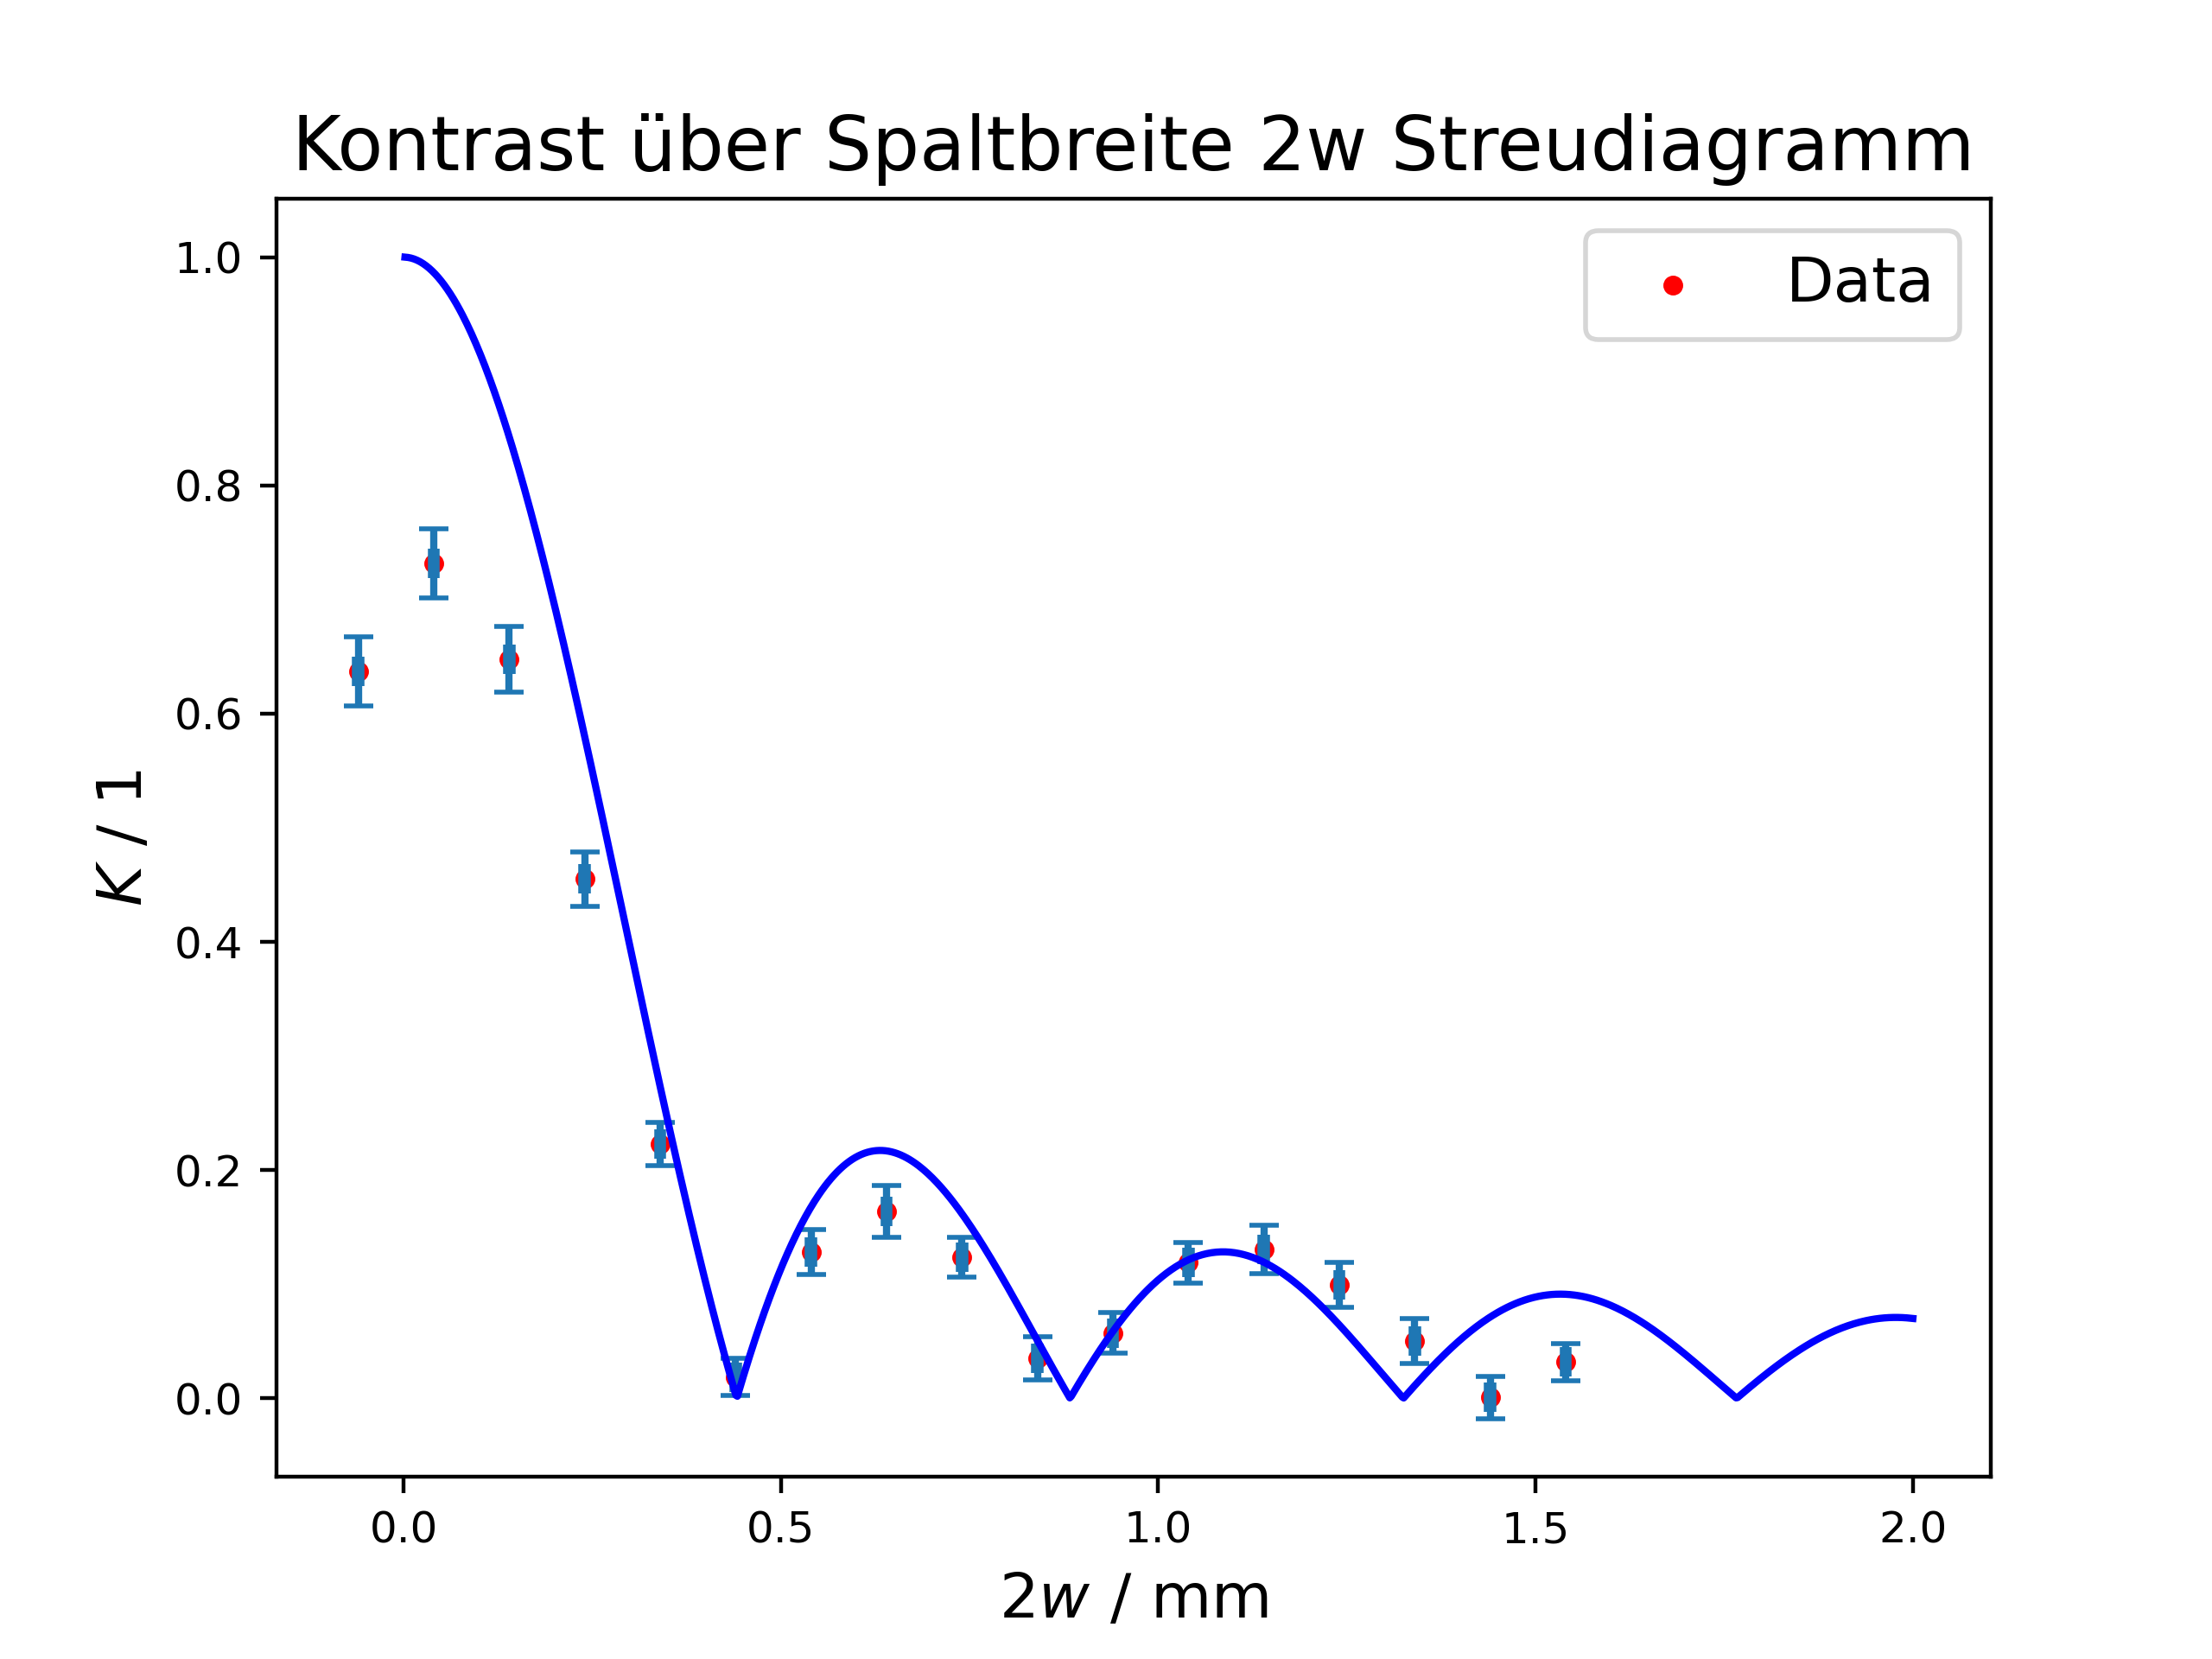
\includegraphics[width=\textwidth]{adj_kontrast}
		\captionbelowof{figure}{Kontrast des Beugungsmusters mit theoretischen Fit
			und gemessenen Werten mit dem Versatz von \SI{0.16}{\mm}}
	\end{minipage}
	\vspace{2mm}
	\begin{minipage}[t]{0.50\textwidth}
		\centering
		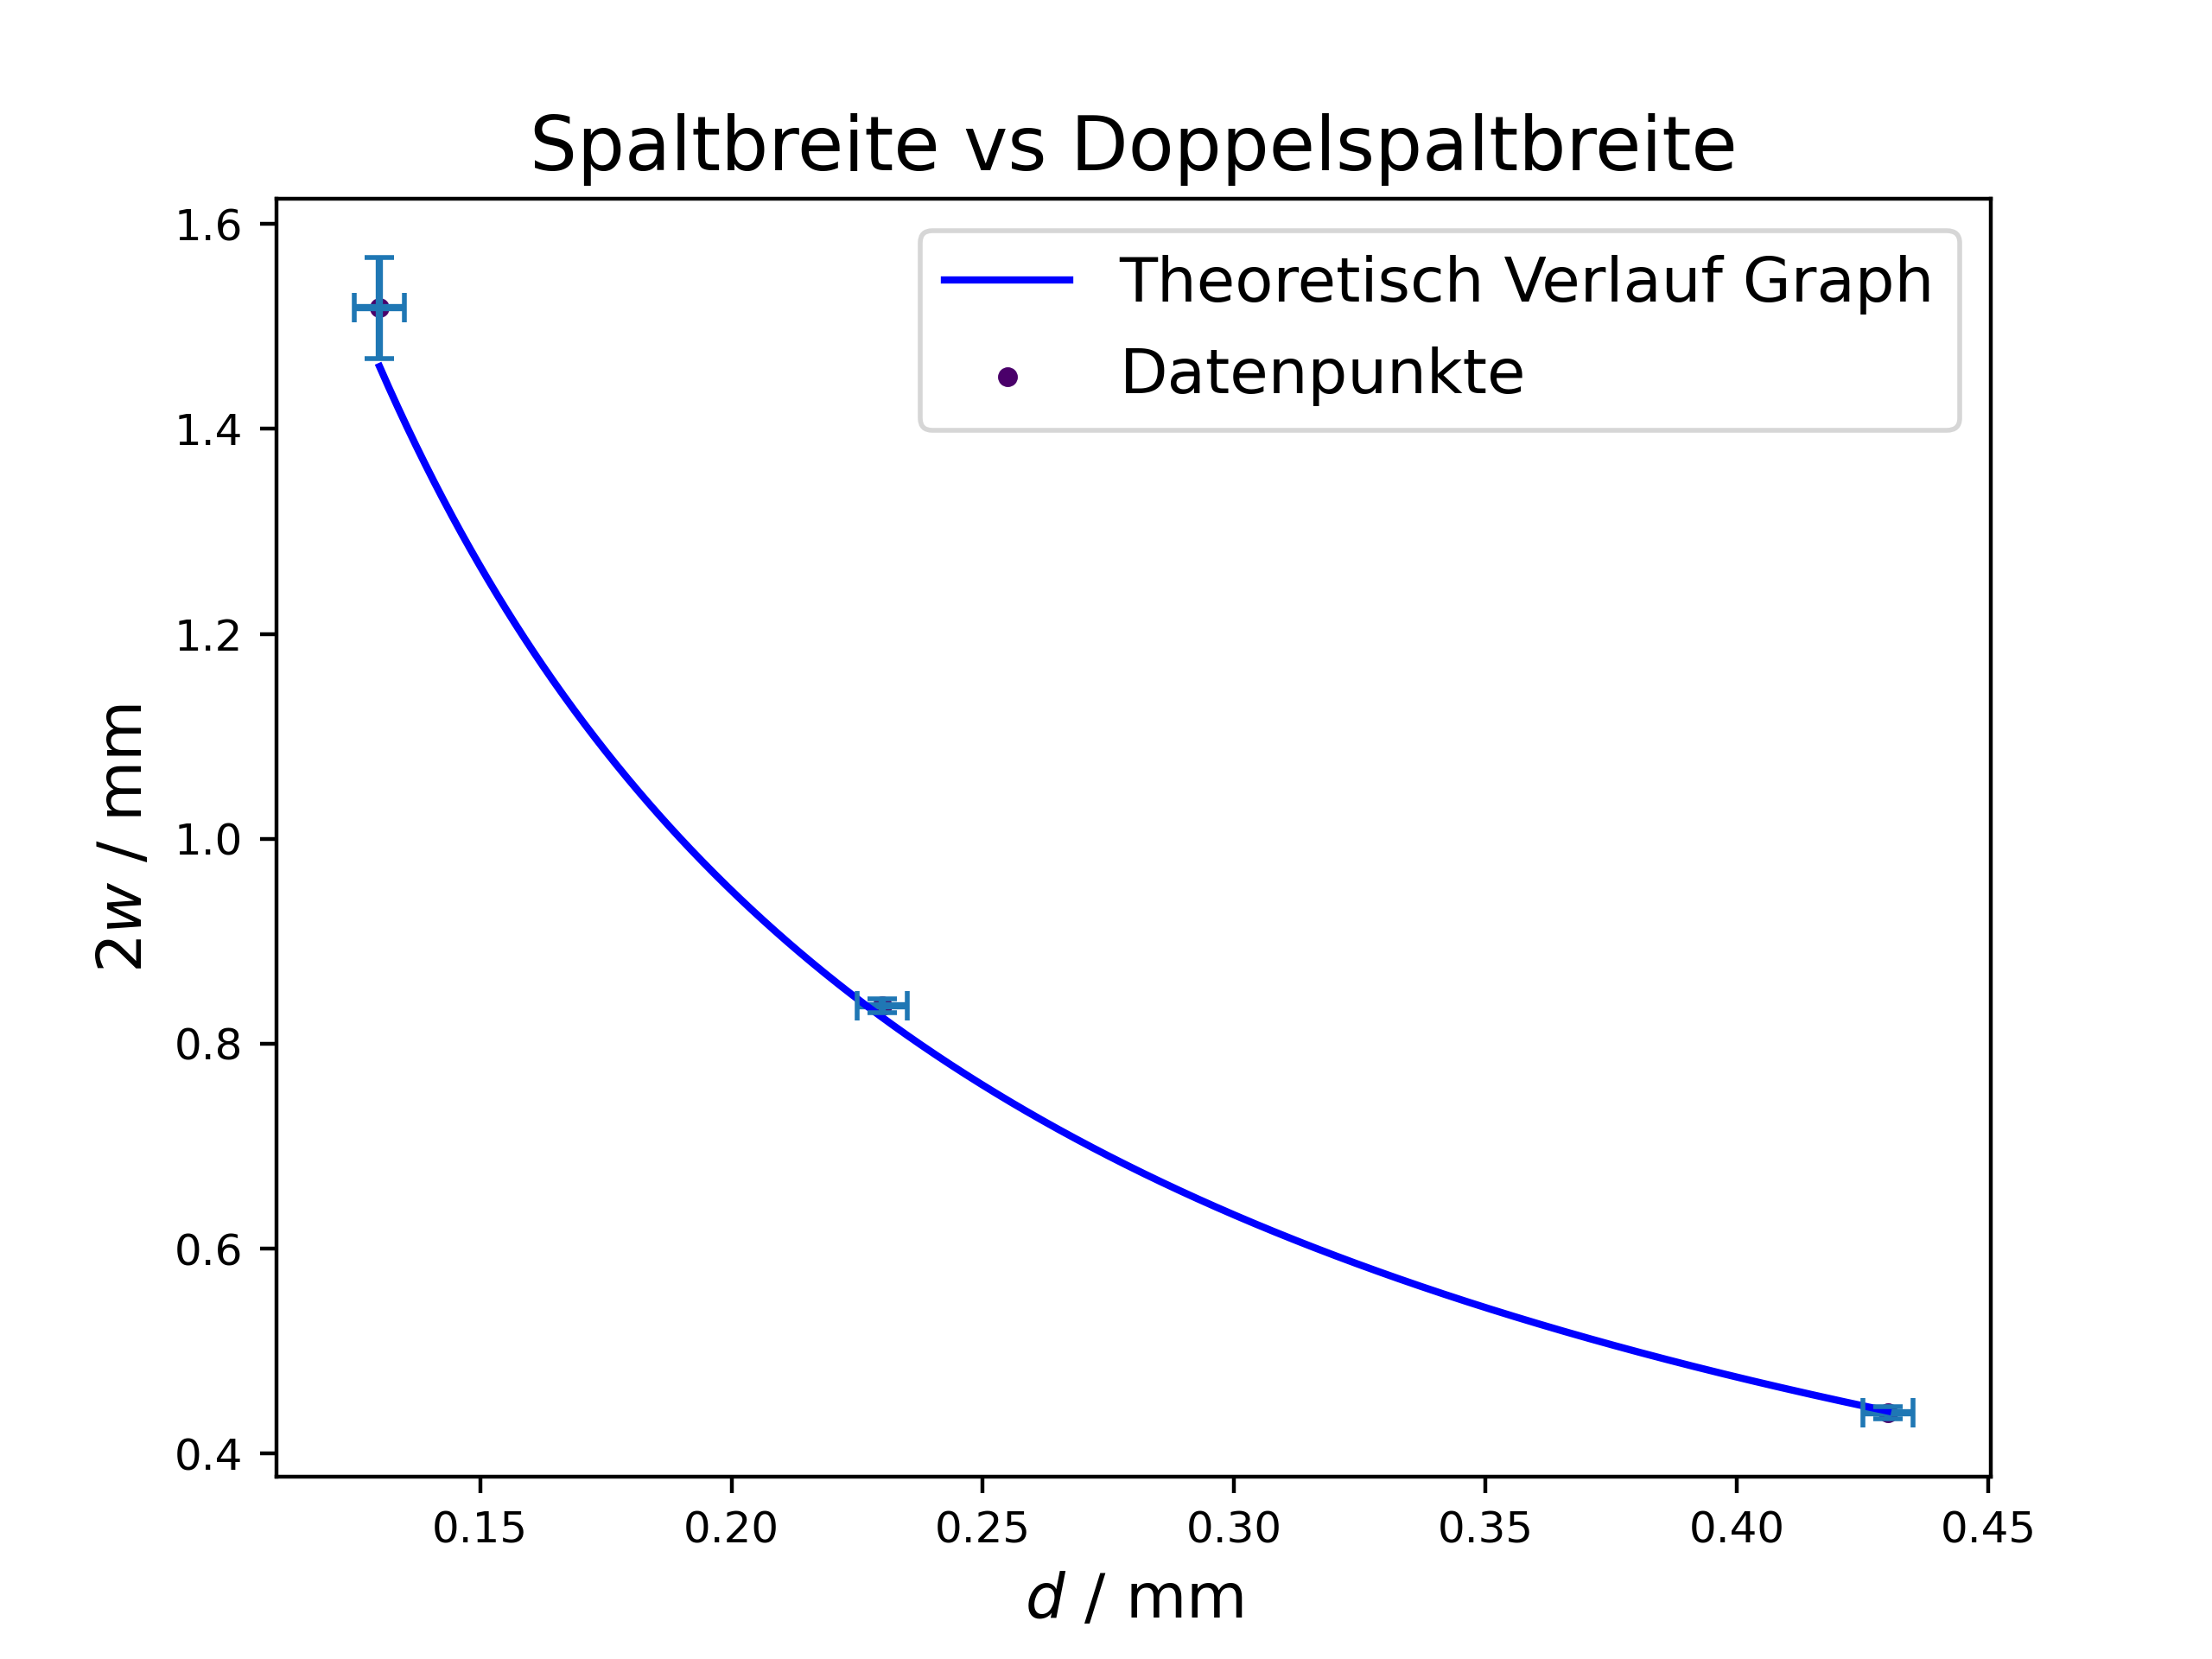
\includegraphics[width=\textwidth]{adj_spaltvsdpspalt}
		\captionof{figure}{Spaltbreite beim ersten Kontrastminimum aufgetragen zur
			Doppelspaltbreite mit dem Versatz von \SI{0.16}{\mm} }
		\label{fig:spaltvsdpspalt_v}
	\end{minipage}
	\vspace{1em}
\end{minipage}

\noindent Besonders beim Betrachten von \autoref{fig:spaltvsdpspalt_v} fällt auf, dass
dieser Versatz annähernd perfekte Wert liefern würde.

\vspace{2mm}

\noindent Ein Verbesserungsvorschlag wäre den Versuch mit einem anderen Aufbau zu
wiederholen, um sicherzustellen, dass der systematische Fehler nicht auf einen
Gerätedefekt oder Aufbaufehler zurückzuführen ist, der , im Gegensatz zum
Versatz der Mikrometerschraube, bislang unbemerkt geblieben ist.

\noindent Eine Mögliche Erklärung dieses Fehlers wäre, dass der Fehler durch die
Überlappung der beiden Blendenteile der Irisblende zustande gekommen ist.

\noindent Ein weiterer Verbesserungsvorschlag wäre die Kamera zu kalibrieren oder
eine Kamera zu verwenden die High-Dynamic-Range hat.

\section{Zusammenfassung}

Sieht man von dem systematischen Fehler ab, liefern die durchgeführten
Versuche, Ergebnisse, die sich mit der Theorie decken. Auch die bestimmte Dicke
der Kunststoffschicht liegt in einer realistischen Größenordnung und ist hier nochmals
angeführt:
\begin{align*}
	t = \SI{530(70)}{\nm}
\end{align*}

%%%



\newpage

\printbibliography
\listoffigures
\listoftables
\end{document}



%Vorlagen
%

%Gleichungen werden so oder mit \begin{equation} formatiert

%Zitate
%\cite{erstes Wort}


%Unterdrücken von Einrücken
%\noindent 

%referenzen
% \aotoref{name}

%für Formeln $ f $
%\subsection{Idealisierungen}

%Gleichung

%\begin{equation}
%	k_{pos} = \frac{4}{300} \frac{V}{\mu\mathrm{s}} = 13333 \, \frac{V}{s}
%\end{equation}

%\begin{align}
%	 \ddot \phi -\frac{g}{l} \cdot \phi &=0 \label{eq:harm}\\
%     \frac{\text{d}^{2}}{\text{dt}^{2}} [\sin(\omega t)]  - \frac{g}{l} \cdot \sin(\omega t) &= 0 \\ 
%     \therefore \quad \omega^{2}&=\frac{g}{l} \label{eq:omega}
%\end{align}


%\begin{align}
%    T &= 2\pi \sqrt{\frac{l}{g}} \label{eq:reg_sqrt} \\
%    T^{2} &= \frac{4\pi^{2}}{g} l \label{eq:reg_lin} 
%\end{align}

%Kompliziertes Bild

%\begin{minipage}{\textwidth}
%\begin{minipage}[t]{0.43\textwidth}
%	\includegraphics[width=\textwidth]{pics/toplot.PNG}
%\end{minipage}
%\begin{minipage}[t]{0.45\textwidth}
%	\includegraphics[width=\textwidth]{pics/bottomlot.PNG}
%\end{minipage}
%	\captionof{figure}{Ansicht von Oben (Rechts) und von Unten (Links) des Senklots}
%	\label{fig:Senklot}
%    \vspace{1em}
%\end{minipage}



%\begin{minipage}{\textwidth}
%\begin{minipage}[t]{0.59\textwidth}
%    \centering
%    \includegraphics[width=\textwidth]{pics/Aufhangung.jpeg}
%    \captionbelowof{figure}{Aufhängung}
%    \label{fig:Aufhaengung}
%\end{minipage}
%\begin{minipage}[t]{0.40\textwidth}
%    \centering
%    \includegraphics[width=\textwidth]{pics/PendelAufbau.png}
%    \captionof{figure}{Versuchsaufbau}
%    \label{fig:Aufbau}
%\end{minipage}
%    \vspace{1em}
%\end{minipage}

%\begin{wrapfigure}[]{r}{0.4\textwidth}
%\begin{tabular}{@{}l@{}}
%\begin{minipage}{\textwidth}
%\includegraphics[width=0.38\textwidth]{pics/Aufhangung.jpeg}
%\noindent \captionbelowof{figure}{Aufhängung}
%\label{fig:Aufhaengung}
%\end{minipage}\\
%\begin{minipage}{\textwidth}
%\includegraphics[width=0.38\textwidth]{pics/PendelAufbau.png}
%\captionof{figure}{Versuchsaufbau}
%\label{fig:Aufbau}
%\end{minipage}
%\end{tabular}
%\end{wrapfigure}


%Tabelle

%\begin{align}
%	\Delta \bar T_{10} &= t \sigma_{\bar T_{10}} + \Delta T_{res} = \frac{t}{\sqrt{N}}\sigma_{T_{10}}+\Delta T_{res}\\
%	\Delta \bar T &= \frac{ \Delta \bar T_{10}}{10}
%\end{align}


%Tabelle
%
%\begin{table}[htbp]
%\centering
%\begin{tabular}{c|c|c|c|l}
%    [$\frac{\text{m}}{\text{s}^{2}}$] & Literaturwert & Wurzel Fit & Linearer Fit &\\ \hline
%    $g$ & \num{9.806191} & \num{9.79} & \num{9.80} &\\
%    $\Delta g$ & \num{1.2e-5} & \num{1e-2}& \num{1e-2} &\\
%\end{tabular}
%	\captionbelowof{table}{Vergleich mit Literaturwert}
%	\label{Tab:Vergleich}
%\end{table}


%\begin{align}
%	& \Delta T_{\phi} = 2\pi \sqrt{ \frac{l}{g} } \frac{\phi^{2}}{16} = 0.0052\,\text{s} 
%\end{align}
